% PRIMITIVITY, THE MANIFOLD AND ITS TANGENT SPACE
\section{Primitivity, the manifold and its tangent space} \label{sec:primitivity_manifold_tangent_space}
Our starting point is a single rank-3 tensor $A \in \mathbb{C}^{D \times d \times D}$, with one leg of \textit{physical dimension} $d$ and two legs of \textit{virtual/bond dimension} $D$. Equivalently, you can see $A$ as a set of $d$ complex matrices $A^s$ of dimension $D \times D$. Completely characterized by $A$, we define the \textit{uniform matrix product state} (uMPS) in the thermodynamic limit as the translation invariant quantum state whose amplitude for orthonormal basis indices $\{s_n\}_{n \in \mathbb{Z}}$ is given by the infinite product of the respective matrices:
\begin{equation} \label{eq:umps}
	\ket{\psi (A)} = \sum_{\{s_n\}} \tbra{v_L} \prod_{n \in \mathbb{Z}} A^{s_n}  \tket{v_R} \ket{\{s_n\}} = \raisebox{-0.55\height}{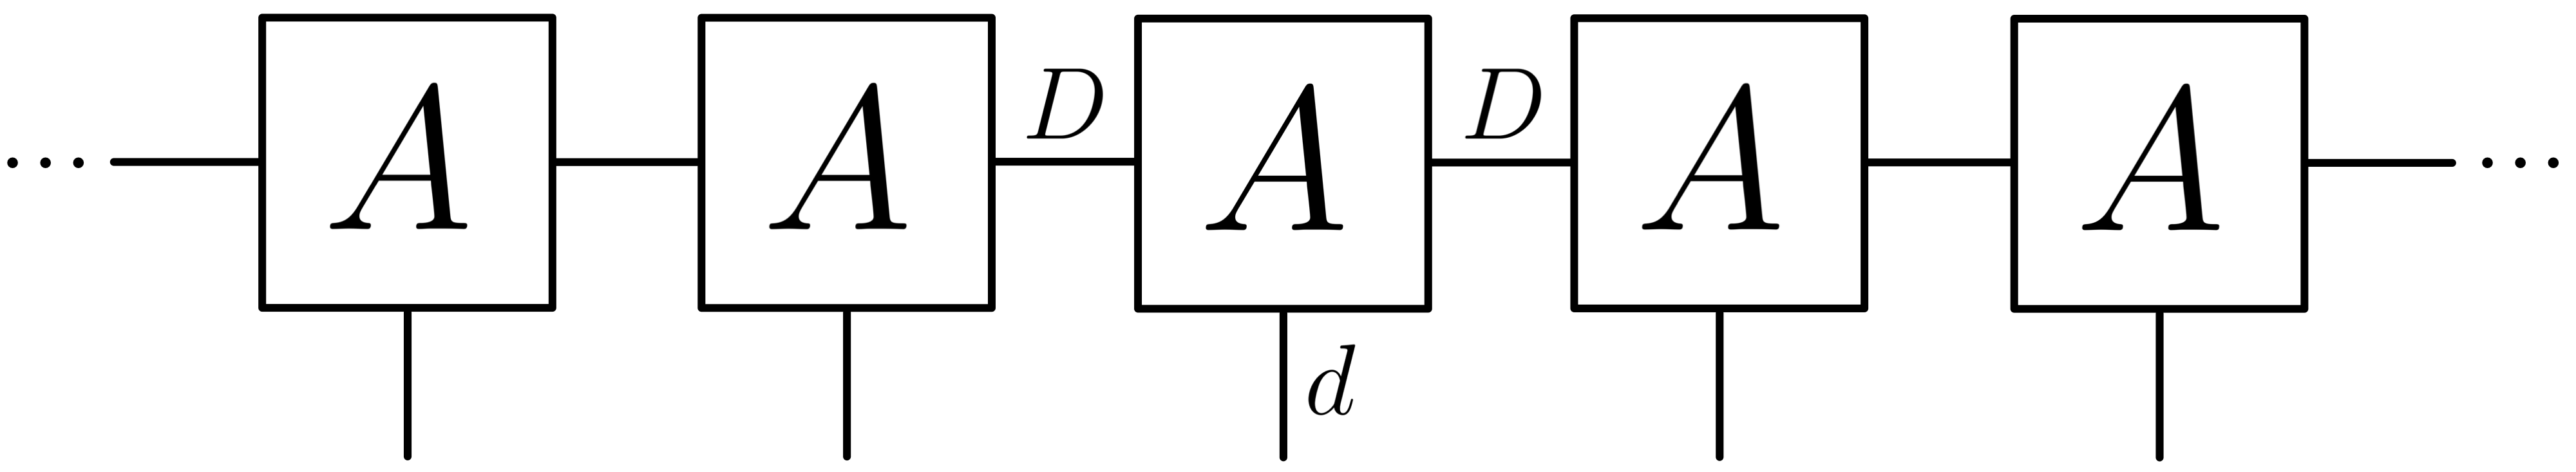
\includegraphics[height=1cm]{umps.png}} \hspace{0.2em}.
\end{equation}
The boundary vectors $\tket{v_L}, \tket{v_R} \in \mathbb{C}^{D}$ ensure normalization and are specified later. \cite{vanderstraeten2019tangent} \\[1em]

% primitivity
\noindent \underline{Primitivity} \\[0.5em]
\noindent The central object that occurs in all important computations (such as norm or local expectation values) is the \textit{transfer matrix} defined as
\begin{equation} \label{eq:transfer_matrix}
	T_A = \sum_{s=1}^d A^s \otimes \overline{A^s} = \raisebox{-0.45\height}{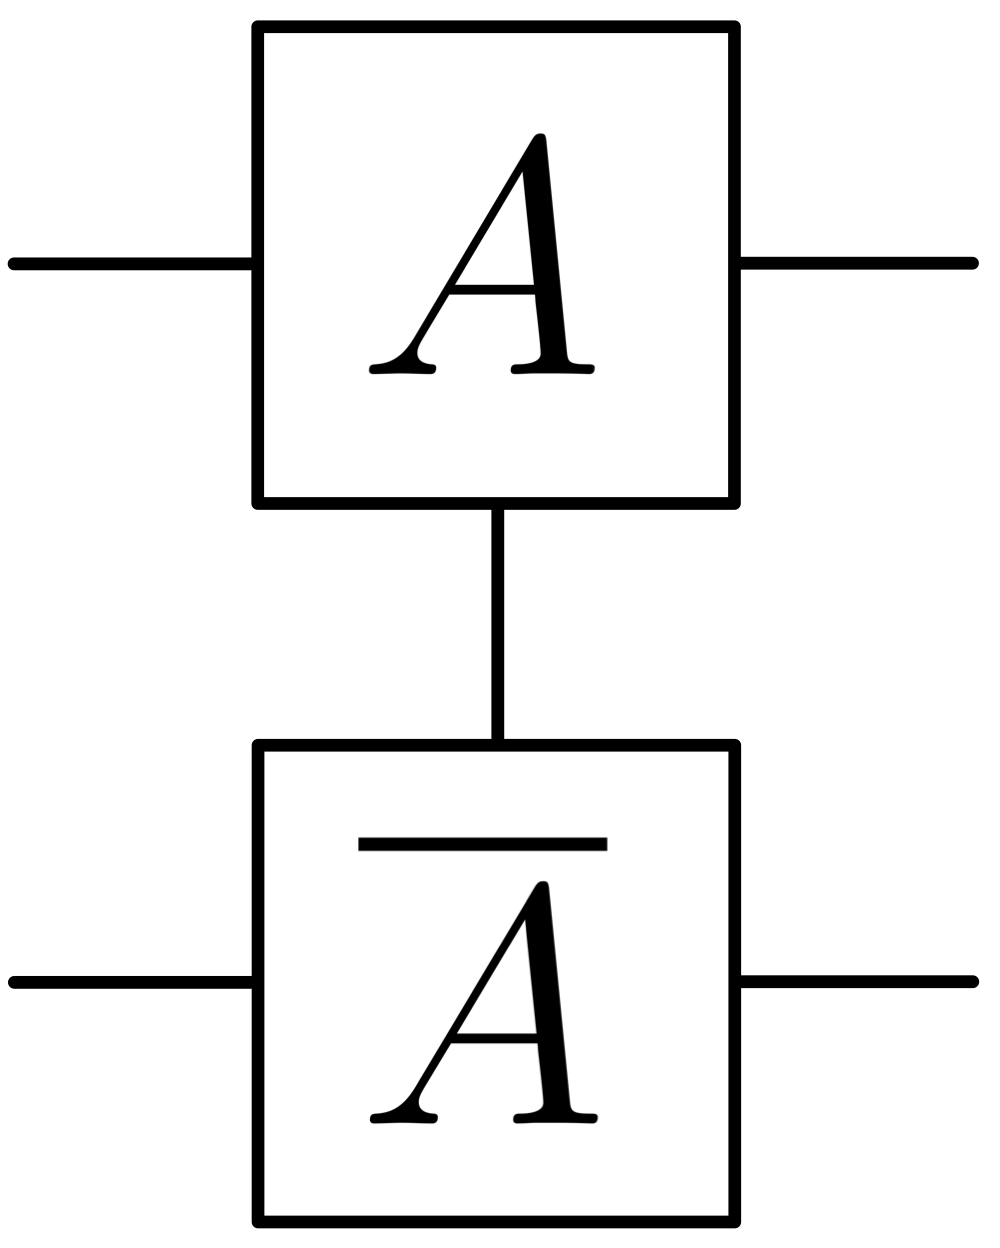
\includegraphics[height=1.6cm]{transfer_matrix.png}} \hspace{0.2em}.
\end{equation}
Using the isomorphism $\tket{\alpha, \beta} \leftrightarrow \tket{\alpha}\tbra{\beta}$ between $\mathbb{C}^{D^2}$ and $\mathbb{C}^{D \times D}$, with the relation
\begin{equation}
	( \gamma, \delta \vert T_A \vert \alpha, \beta ) = ( \gamma \vert \mathcal{E}_A( \tket{\alpha} \tbra{\beta} ) \vert \delta ),
\end{equation}
we can see $T_A$ as a matrix representation of the linear map $\mathcal{E}_A: \mathbb{C}^{D \times D} \rightarrow \mathbb{C}^{D \times D}$, mapping matrices $X$ to
\begin{equation} \label{eq:quantum_channel}
	\mathcal{E}_A(X) =  \sum_{s=1}^d A^s X {A^s}^{\dagger} = \raisebox{-0.55\height}{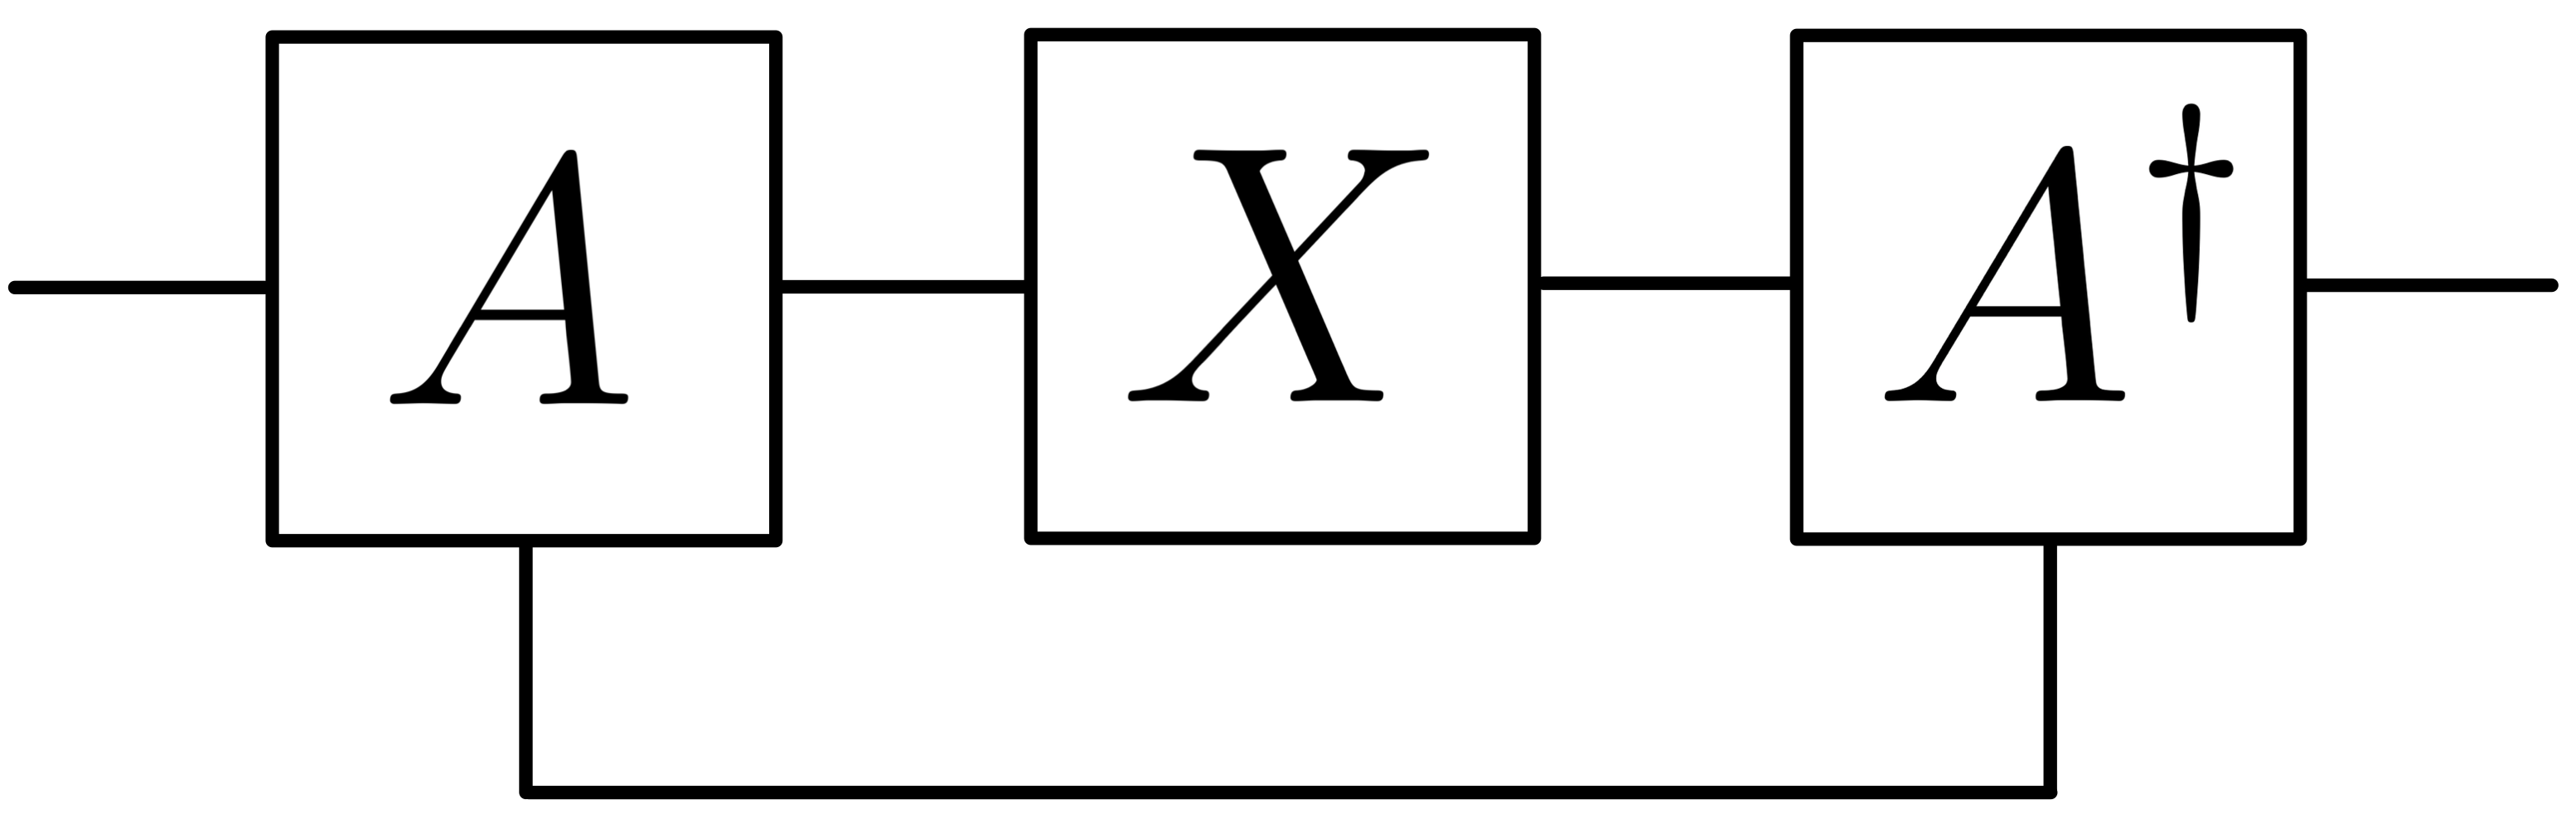
\includegraphics[height=1cm]{quantum_channel.png}} \hspace{0.2em}.
\end{equation}
This is known as the \textit{Kraus representation} of a \textit{completely positive}\footnote{A linear map $\mathcal{E}: \mathbb{C}^{D \times D} \rightarrow \mathbb{C}^{D \times D}$ is called \textit{positive} if it maps positive semidefinite matrices to positive semidefinite matrices, i.e. if $\mathcal{E}(X) \geq 0$ for all $X \geq 0$. It is called \textit{completely positive} if $\mathcal{E} \otimes \mathrm{id}_n$ is positive for all $n \in \mathbb{N}$, where $\mathrm{id}_n$ is the identity map on $\mathbb{C}^{n \times n}$ such that $\mathcal{E} \otimes \mathrm{id}_n: X \otimes Y \mapsto \mathcal{E}(X) \otimes Y$.} map. If $\mathcal{E}_A$ is in addition \textit{trace preserving}, it describes a \textit{quantum channel}, mapping density matrices to density matrices. In appendix \ref{ch:quantum_channels_mps} we elaborate on the relation between uMPS and quantum channels  \cite{wolf2012channels}. In particular, on the crucial spectral property of \textit{primitivity}. After having ensured that $T_A$ has \textit{spectral radius}\footnote{The spectral radius is defined as $\rho = \mathrm{max}\{\vert \lambda \vert \: \vert \: T_A \tket{X} = \lambda \tket{X} \text{ for some nonzero } X \in \mathbb{C}^{D \times D}\}$.} $\rho = 1$ (by rescaling $A \rightarrow A / \sqrt{\rho}$ if $\rho \neq 1$), we call $T_A$ \textit{primitive} if, counting algebraic multiplicities, there is only one dominant eigenvalue of magnitude and value 1 and the corresponding left and right eigenvectors $r, l$ are positive definite and normalized to $\mathrm{tr}[l^T r] = 1$:
\begin{equation} \label{eq:primitive_transfer_matrix}
	T_A = \tket{r}\tbra{l} + \mathcal{O}(\vert \lambda_2 \vert) \text{ with } \vert \lambda_2 \vert < 1, \: r, l > 0 \text{ and } (l \vert r ) = 1.
\end{equation}
We prove in appendix \ref{ch:quantum_channels_mps}, that primitivity of $T_A$ is equivalent to the existence of a finite \textit{injectivity length} $L_0 \in \mathbb{N}$ such that for all $L \geq L_0$ the products $A^{s_1} \cdots A^{s_L}$ span the whole space of $D \times D$ matrices:
\begin{equation}
	\mathrm{span}\{A^{s_1} \cdots A^{s_L}\}_{s_1, \ldots, s_L} = \mathbb{C}^{D \times D}.
\end{equation}
For $d$ randomly drawn matrices $\{A^s\}_{s=1}^d$, the dimension of $\mathrm{span}\{A^{s_1} \cdots A^{s_L}\}_{s_1, \ldots, s_L}$ is expected to grow as $d^L$ until it reaches $D^2$. Therefore, a generic tensor is expected to be primitive with $L_0 \sim 2 \ln D / \ln d$, whereas non-primitive tensors appear with measure zero in the space $\mathbb{C}^{D \times d \times D}$. \cite{perez2007matrix} \\[0.5em]

\noindent Using \eqref{eq:primitive_transfer_matrix}, we can reduce the uMPS overlap to the overlaps of the boundary vectors with the fixed points of $T_A$:
\begin{equation}
	\langle \psi (\overline{A}) \vert \psi (A) \rangle = \tbra{v_L, \overline{v_L}} \lim_{N \to \infty} T_A^{N} \tket{v_R, \overline{v_R}} = ( v_L, \overline{v_L} \vert r ) ( l \vert v_R, \overline{v_R} ) \overset{!}{=} 1.
\end{equation}
We formally choose $v_L$ and $v_R$ such that these overlaps equal unity, but they don't have any effect on the bulk properties of $\ket{\psi (A)}$ and we will not mention them anymore in the following. \\[1em]

% manifold
\noindent \underline{The manifold} \\[0.5em]
\noindent There exists a \textit{gauge freedom} in the choice of the tensor representation $A$ of a physical state $\ket{\psi (A)}$. It is easy to convince yourself that the \textit{similarity transformation} $B^s = S A^s S^{-1}$\footnote{With a slight abuse of notation, we often denote the matrix-wise similarity transformation $S A^s S^{-1}$ for all $s$ as $S A S^{-1}$.}, for any invertible matrix $S \in \mathbb{C}^{D \times D}$, leaves the uMPS invariant: $\ket{\psi (A)} = \ket{\psi (B)}$. It can be proven\footnote{and with the \textit{fundamental theorem} \ref{thm:fundamental_theorem} we do, but under the assumption of primitivity and unitality, which requires S to be unitary.} that this is in fact the only such transformation:
\begin{equation} \label{eq:umps_gauge}
	\ket{\psi (A)} = \ket{\psi (B)} \text{ if and only if } B^s = S A^s S^{-1} \text{ for } S \in \mathrm{GL}(D, \mathbb{C}).
\end{equation}
Since matrices $S$ which are scalar multiples of the identity have a trivial effect, the effective \textit{gauge group} is not the \textit{general linear group} $\mathrm{GL}(D, \mathbb{C})$ but the \textit{projective general linear group} $\mathrm{PGL}(D, \mathbb{C}) = \mathrm{GL}(D, \mathbb{C}) / \mathrm{GL}(1, \mathbb{C})$. For fixed bond dimension $D$, the \textit{complex manifold} of primitive tensors modulo gauge is then given by
\begin{equation}
	\mathcal{A}_D = \{A \in \mathbb{C}^{D \times d \times D} \: \vert \: T_A \text{ is primitive} \} / \mathrm{PGL}(D, \mathbb{C}). 
\end{equation}
The primitivity property ensures that this quotient space is \textit{biholomorphic}\footnote{A map between complex manifolds is \textit{biholomorphic} if it is a bijective holomorphic map whose inverse is also holomorphic.} to the corresponding set of uMPS,
\begin{equation}
	\mathcal{M}_D = \{ \ket{\psi (A)} \in \mathcal{H} \: \vert \: A \in \mathcal{A}_D\},	
\end{equation}
turning it into a smooth, low-dimensional manifold in the exponentially large Hilbert space $\mathcal{H}$ of $d$-dimensional spins on an infinite chain. We will see in the next section \ref{sec:canonical_form_area_law}, that within $\mathcal{M}_D$ we can faithfully approximate ground states of local, gapped Hamiltonians. \\[1em]

% tangent space
\noindent \underline{The tangent space} \\[0.5em]
\noindent Since the sum of two uMPS with bond dimension $D$ clearly does not remain within $\mathcal{M}_D$, the manifold $\mathcal{M}_D$ is non-linear. However, as for any smooth manifold, we can assign a linear \textit{tangent space} $\mathcal{T}_{\ket{\psi (A)}}$ to each point $\ket{\psi (A)} \in \mathcal{M}_D$. It consists of all states obtained by infinitesimal variations of the tensor $A$:
\begin{equation} \label{eq:tangent_space_vector}
	\ket{\psi (B; A)} = \sum_{\alpha, s, \beta} B^s_{\alpha, \beta} \left[ \partial_{A^s_{\alpha, \beta}}\ket{\psi (A)} \right] = \sum_n \raisebox{-0.45\height}{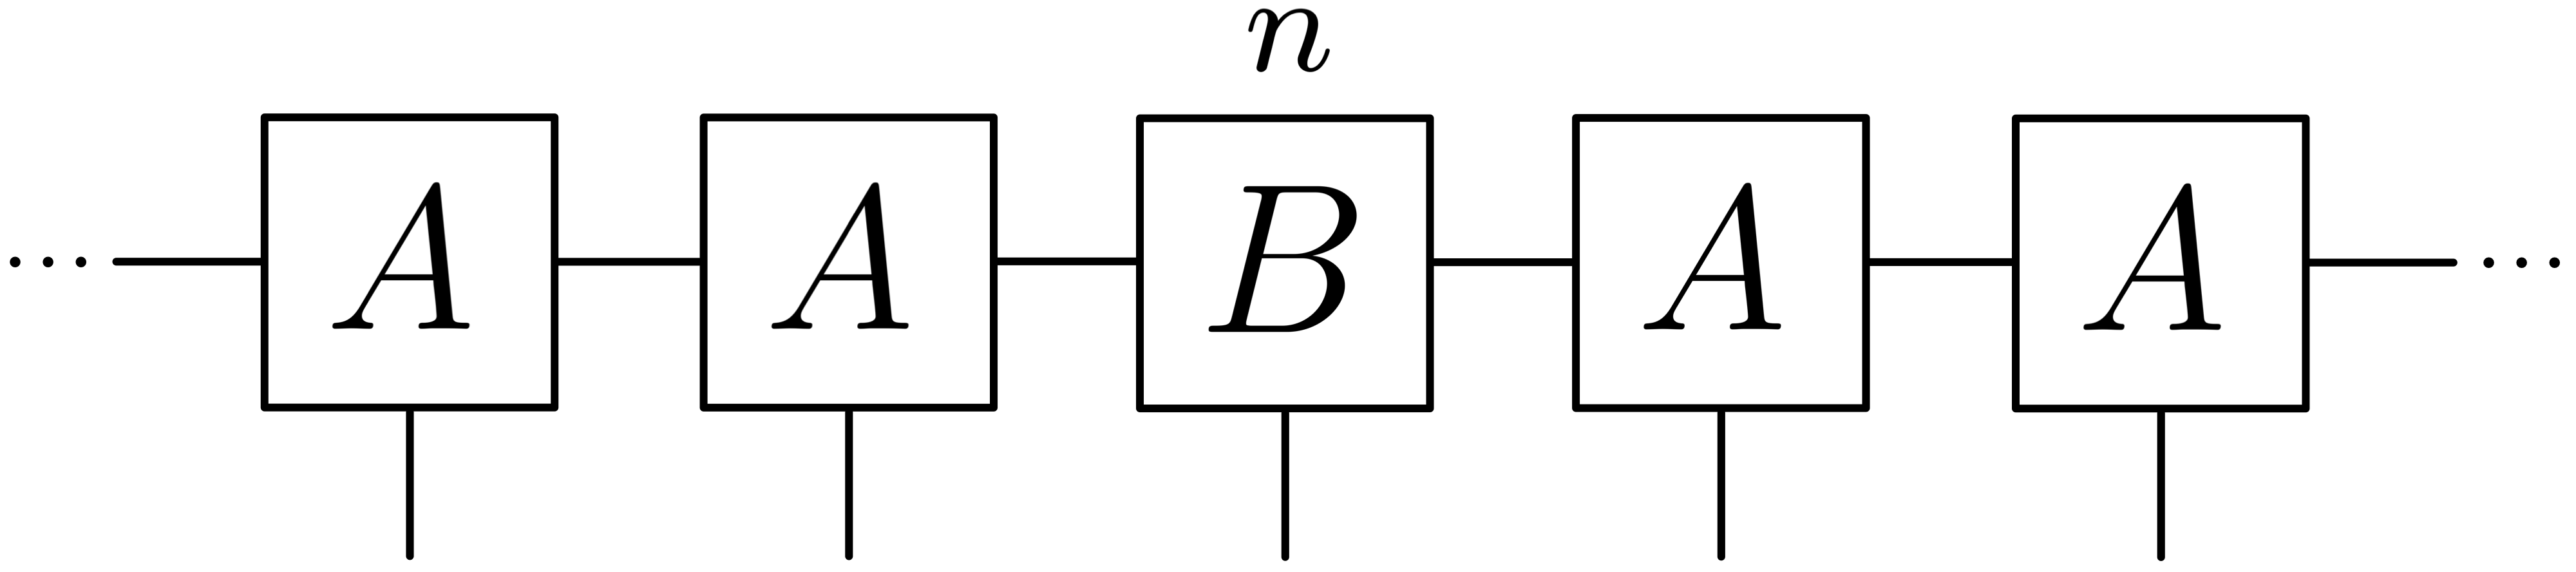
\includegraphics[height=1.2cm]{tangent_vector.png}} \hspace{0.2em}.
\end{equation}
In section \ref{sec:uexcitations}, this will be the space in which the quasiparticle excitations on top of the ground state vacuum live. In figure \ref{fig:manifold_tangent_space} we illustrate the mapping of tensors to uMPS, the manifold and its tangent space. \cite{haegeman2014geometry, haegeman2013post}
\begin{figure}[t]
  \centering
  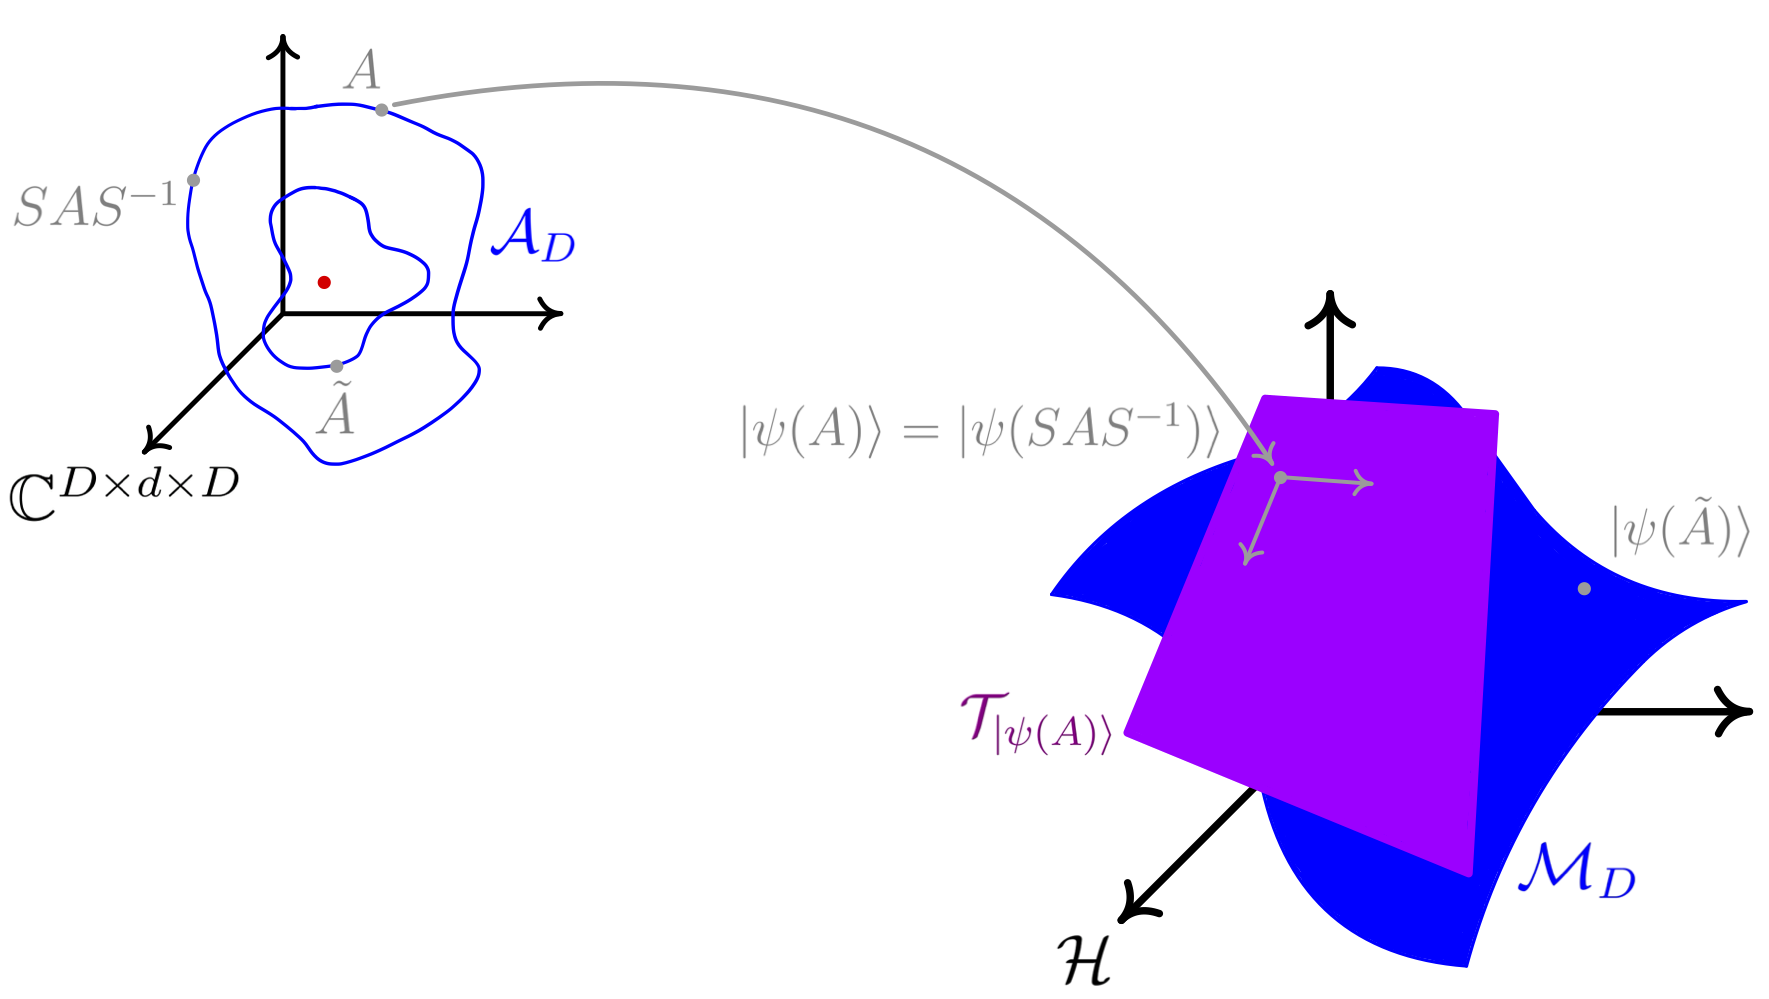
\includegraphics[width=0.75\linewidth]{manifold_tangent_space.png}
  \caption{Illustration of the uMPS manifold and its tangent space. Tensors from parameter space $\mathbb{C}^{D \times d \times D}$ are mapped to physical states in Hilbert space $\mathcal{H}$. The actual tensor manifold $\mathcal{A}_D$ is defined modulo gauge orbits. The red dot in the middle corresponds to a tensor of measure zero whose transfer matrix is not primitive. It has to be excluded from $\mathcal{A}_D$ to define a so called \textit{principal fiber bundle}. The uniform matrix product states then form a smooth, nonlinear manifold $\mathcal{M}_D$ within the Hilbert space. To each point $\ket{\psi (A)}$ we can assign a linear tangent space $\mathcal{T}_{\ket{\psi (A)}}$ consisting of all states obtained by infinitesimal variations $\ket{\psi (B; A)}$. \cite{haegeman2014geometry, haegeman2013post}}
  \label{fig:manifold_tangent_space}
\end{figure}


% INTRINSIC CANONICAL FORM AND AREA LAW
\section{Intrinsic canonical form and area law} \label{sec:canonical_form_area_law}
Within the gauge freedom $S A S^{-1}$, we want to bring the uMPS \eqref{eq:umps} into a \textit{canonical form} that ensures orthonormality in a bipartition and numerical stability in the variational algorithms of sections \ref{sec:vumps}, \ref{sec:uexcitations}. \\[1em]

% canonical form
\noindent \underline{Canonical form} \\[0.5em]
\noindent More precisely, we want to find invertible $L, R \in \mathbb{C}^{D \times D}$ such that
\begin{equation} \label{eq:left_gauge}
	A_L = L A L^{-1} \text{ is left isometric: } \tbra{\mathbbm{1}} T_{A_L} = \tbra{\mathbbm{1}},
\end{equation}
\begin{equation} \label{eq:right_gauge}
	A_R = R^{-1} A R \text{ is right isometric: } T_{A_R} \tket{\mathbbm{1}}  = \tket{\mathbbm{1}}.
\end{equation}
At this point it is useful to introduce the \textit{dual map} $\mathcal{E}^*_A$ of \eqref{eq:quantum_channel}, which is defined via $\mathrm{tr}[\mathcal{E}_A(X) Y] = \mathrm{tr}[X \mathcal{E}^*_A(Y)]$ for all $X, Y \in \mathbb{C}^{D \times D}$. It has the Kraus representation 
\begin{equation}
	\mathcal{E}^*_A(Y) =  \sum_{s=1}^d {A^s}^{\dagger} Y A^s,
\end{equation}
and the matrix representation $T_A^{\dagger}$, so that $T_A^{\dagger} \tket{Y} = \tket{\mathcal{E}^*_A(Y)}$. With our transpose-only bra notation this corresponds to $\tbra{Y} T_A = \overline{\tbra{\mathcal{E}^*_A(\overline{Y})}}$. From this we can conclude for the left fixed point $l$:
\begin{equation} \label{eq:left_fixed_point_dual}
	\tbra{l} T_A = \tbra{l} \text{ if and only if } \mathcal{E}^*_A(\overline{l}) = \overline{l}. \\
\end{equation}
Since $\overline{l}$ is positive definite, we can take its square root and the inverse thereof. Knowing this we define
\begin{equation} \label{eq:AL_from_square_root}
	A_L = \overline{l}^{1/2} A \overline{l}^{-1/2} \text{ to fulfill } \mathcal{E}^*_{A_L}(\mathbbm{1}) =  \sum_{s} {A^s_L}^{\dagger} A^s_L =  \overline{l}^{-1/2} \left( \sum_{s} {A^s}^{\dagger} \overline{l} A^s \right) \overline{l}^{-1/2} = \mathbbm{1}.
\end{equation}
 Similarly, we can take square root and inverse of the positive definite right fixed point $r$ and define 
 \begin{equation} \label{eq:AR_from_square_root}
 	A_R = r^{-1/2} A r^{1/2} \text{ to fulfill } \mathcal{E}_{A_R} (\mathbbm{1}) = \sum_s A_R^s {A_R^s}^{\dagger} = r^{-1/2} \left( \sum_s A^s r {A^s}^{\dagger} \right) r^{-1/2} = \mathbbm{1}. 
 \end{equation}
In practice, computing $A_L$ and $A_R$ according to \eqref{eq:AL_from_square_root} and \eqref{eq:AR_from_square_root} is suboptimal due to a potentially ill-conditioned inversion of small eigenvalues of $\overline{l}^{1/2}$ and $r^{1/2}$. Instead, we iteratively solve the equations $L A = A_L L$ and $A R = R A_R$ with QR and LQ decompositions. Making the decompositions unique (by ensuring positive values on the main diagonal of the triangular matrices), we can reach convergence up to arbitrary tolerance tol: 
\begin{equation} \label{eq:iterative_qr}
	\raisebox{-0.6\height}{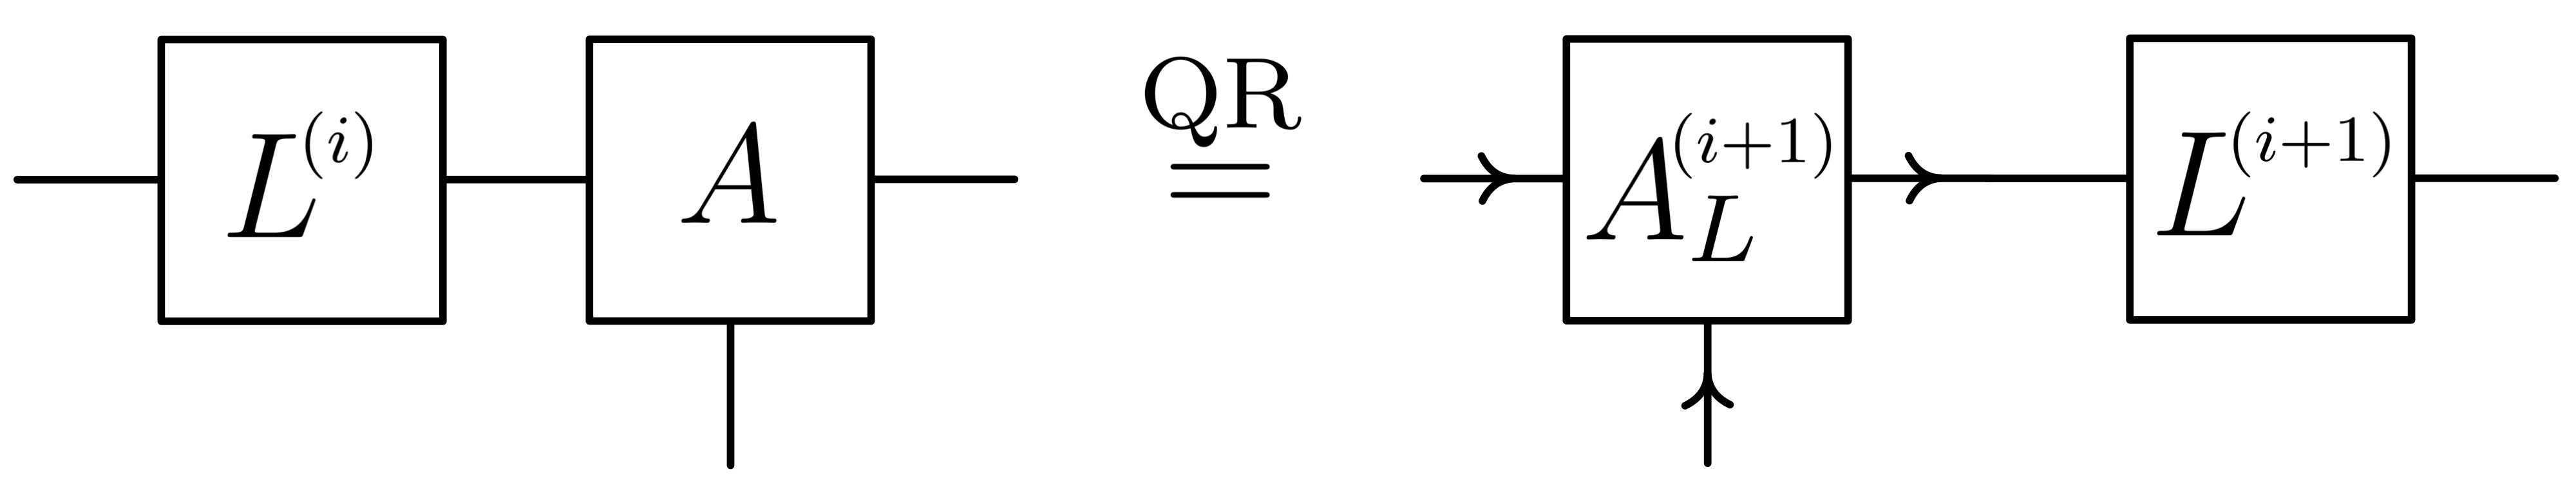
\includegraphics[height=1.4cm]{iterative_qr.png}} \:\: \text{ until } \Vert L^{(i+1)} - L^{(i)} \Vert_2 < \mathrm{tol}, 
\end{equation}
\begin{equation}
	\raisebox{-0.6\height}{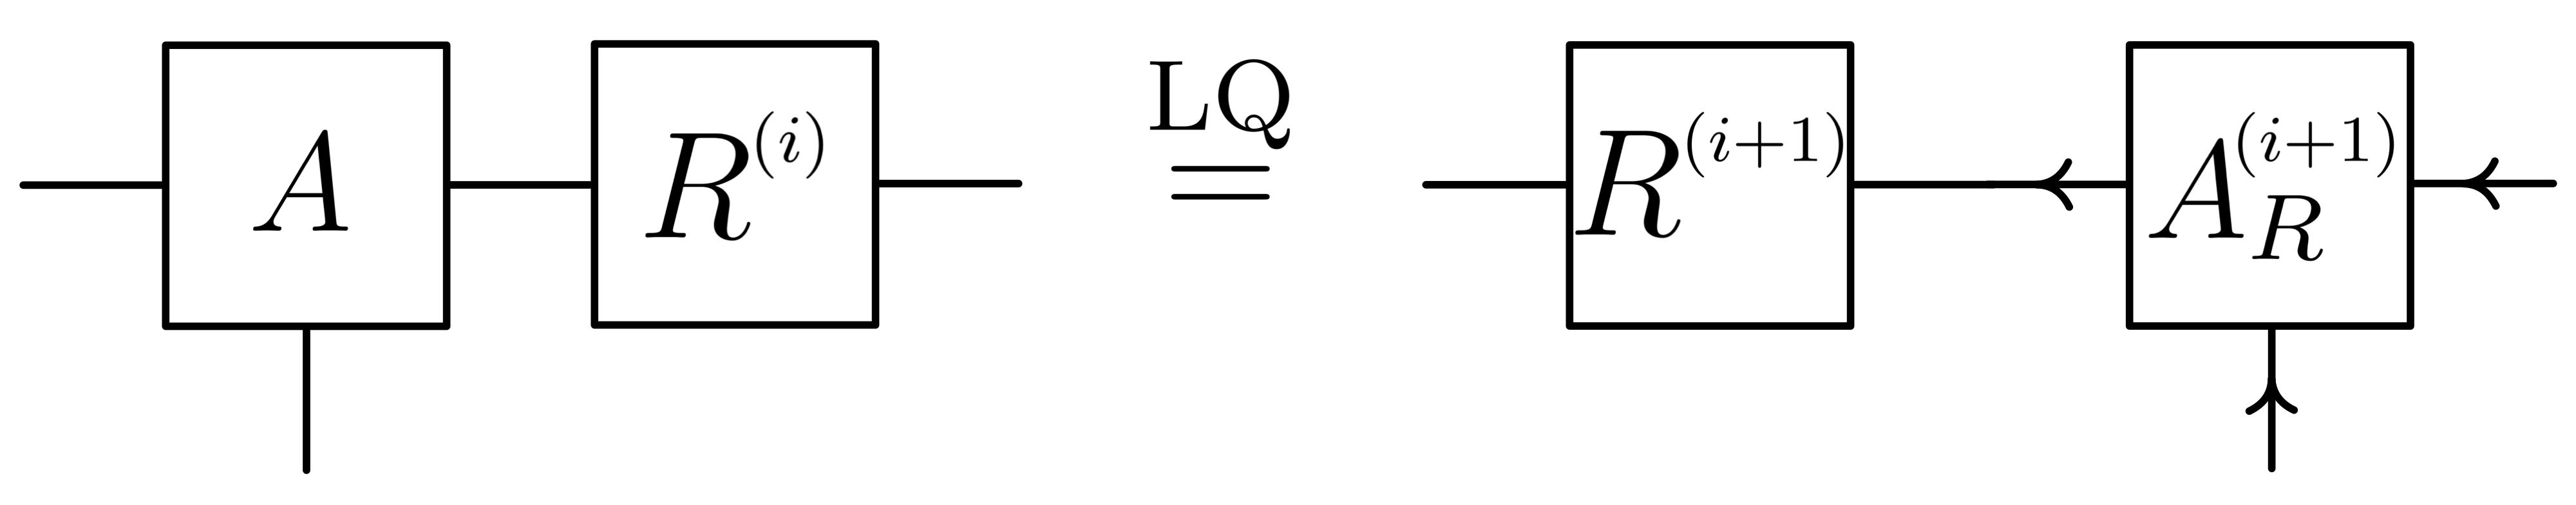
\includegraphics[height=1.4cm]{iterative_lq.png}} \:\: \text{ until } \Vert R^{(i+1)} - R^{(i)} \Vert_2 < \mathrm{tol}.
\end{equation}
For any bond $n$ in the uMPS, we can install the left isometric gauge \eqref{eq:left_gauge} for all tensors on the left and the right isometric gauge \eqref{eq:right_gauge} for all tensors on the right. It remains a \textit{center matrix} $C = LR$ at the chosen bond, that relates $A_L$ and $A_R$ via $A_L C = L A R = C A_R$. We decompose $C$ with an SVD into $C = U S V$ and redefine $C \rightarrow S / \Vert S \Vert_2$, which normalizes the uMPS and makes the center matrix diagonal positive definite. The isometric tensors are accordingly redefined as $A_L \rightarrow U^{\dagger} A_L U$ and $A_R \rightarrow V A_R V^{\dagger}$. Since both $U$ and $V$ are unitary matrices, i.e. satisfy $U^{\dagger}U = UU^{\dagger} = \mathbbm{1}$, $VV^{\dagger} = V^{\dagger}V = \mathbbm{1}$, all desired properties are preserved. Sometimes it is useful to summarize $A_L$ and $C$ (or equivalently $C$ and $A_R$) into a normalized \textit{center tensor} $A_C$. \\[0.5em]

\noindent In total, we derived the following \textit{canonical form} for a uMPS $\ket{\psi (A)} \in \mathcal{M}_D$:
\begin{equation} \label{eq:umps_canonical_form}
	\raisebox{-0.5\height}{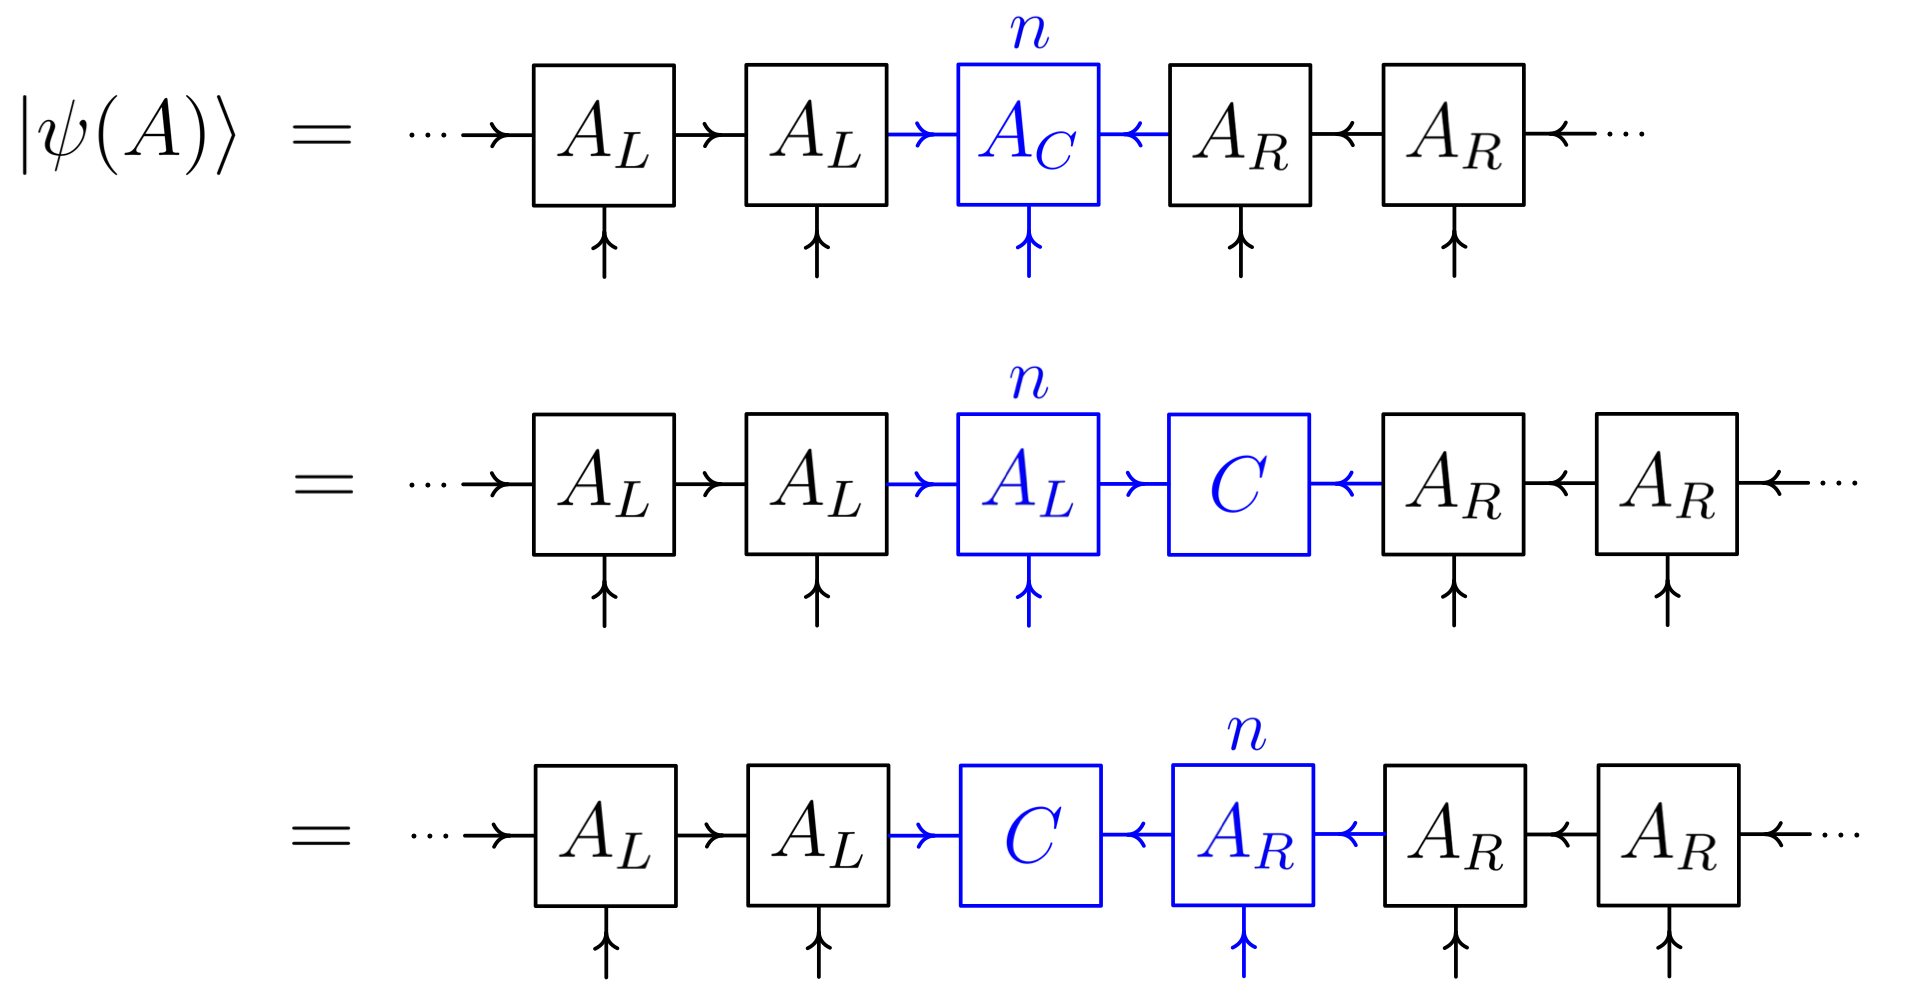
\includegraphics[height=5.5cm]{umps_canonical_form.png}}
\end{equation}
In practice, the four tensors $A_L$, $A_R$, $C$ and $A_C$ are the central attributes of a uMPS class. \\[1em]

% area law
\noindent \underline{Area law} \\[0.5em]
\noindent As a first application of the canonical form, we want to investigate the role of the bond dimension $D$. We can see \eqref{eq:umps_canonical_form} as a bipartition between all spins on the left and on the right of bond $n$:
\begin{equation}
	\ket{\psi (A)} = \sum_{\alpha = 1}^D C_{\alpha} \ket{\psi(A_L)_{\alpha}} \ket{\psi(A_R)_{\alpha}}.
\end{equation}
Since the states 
\begin{equation}
	\ket{\psi(A_L)_{\alpha}} = \raisebox{-0.55\height}{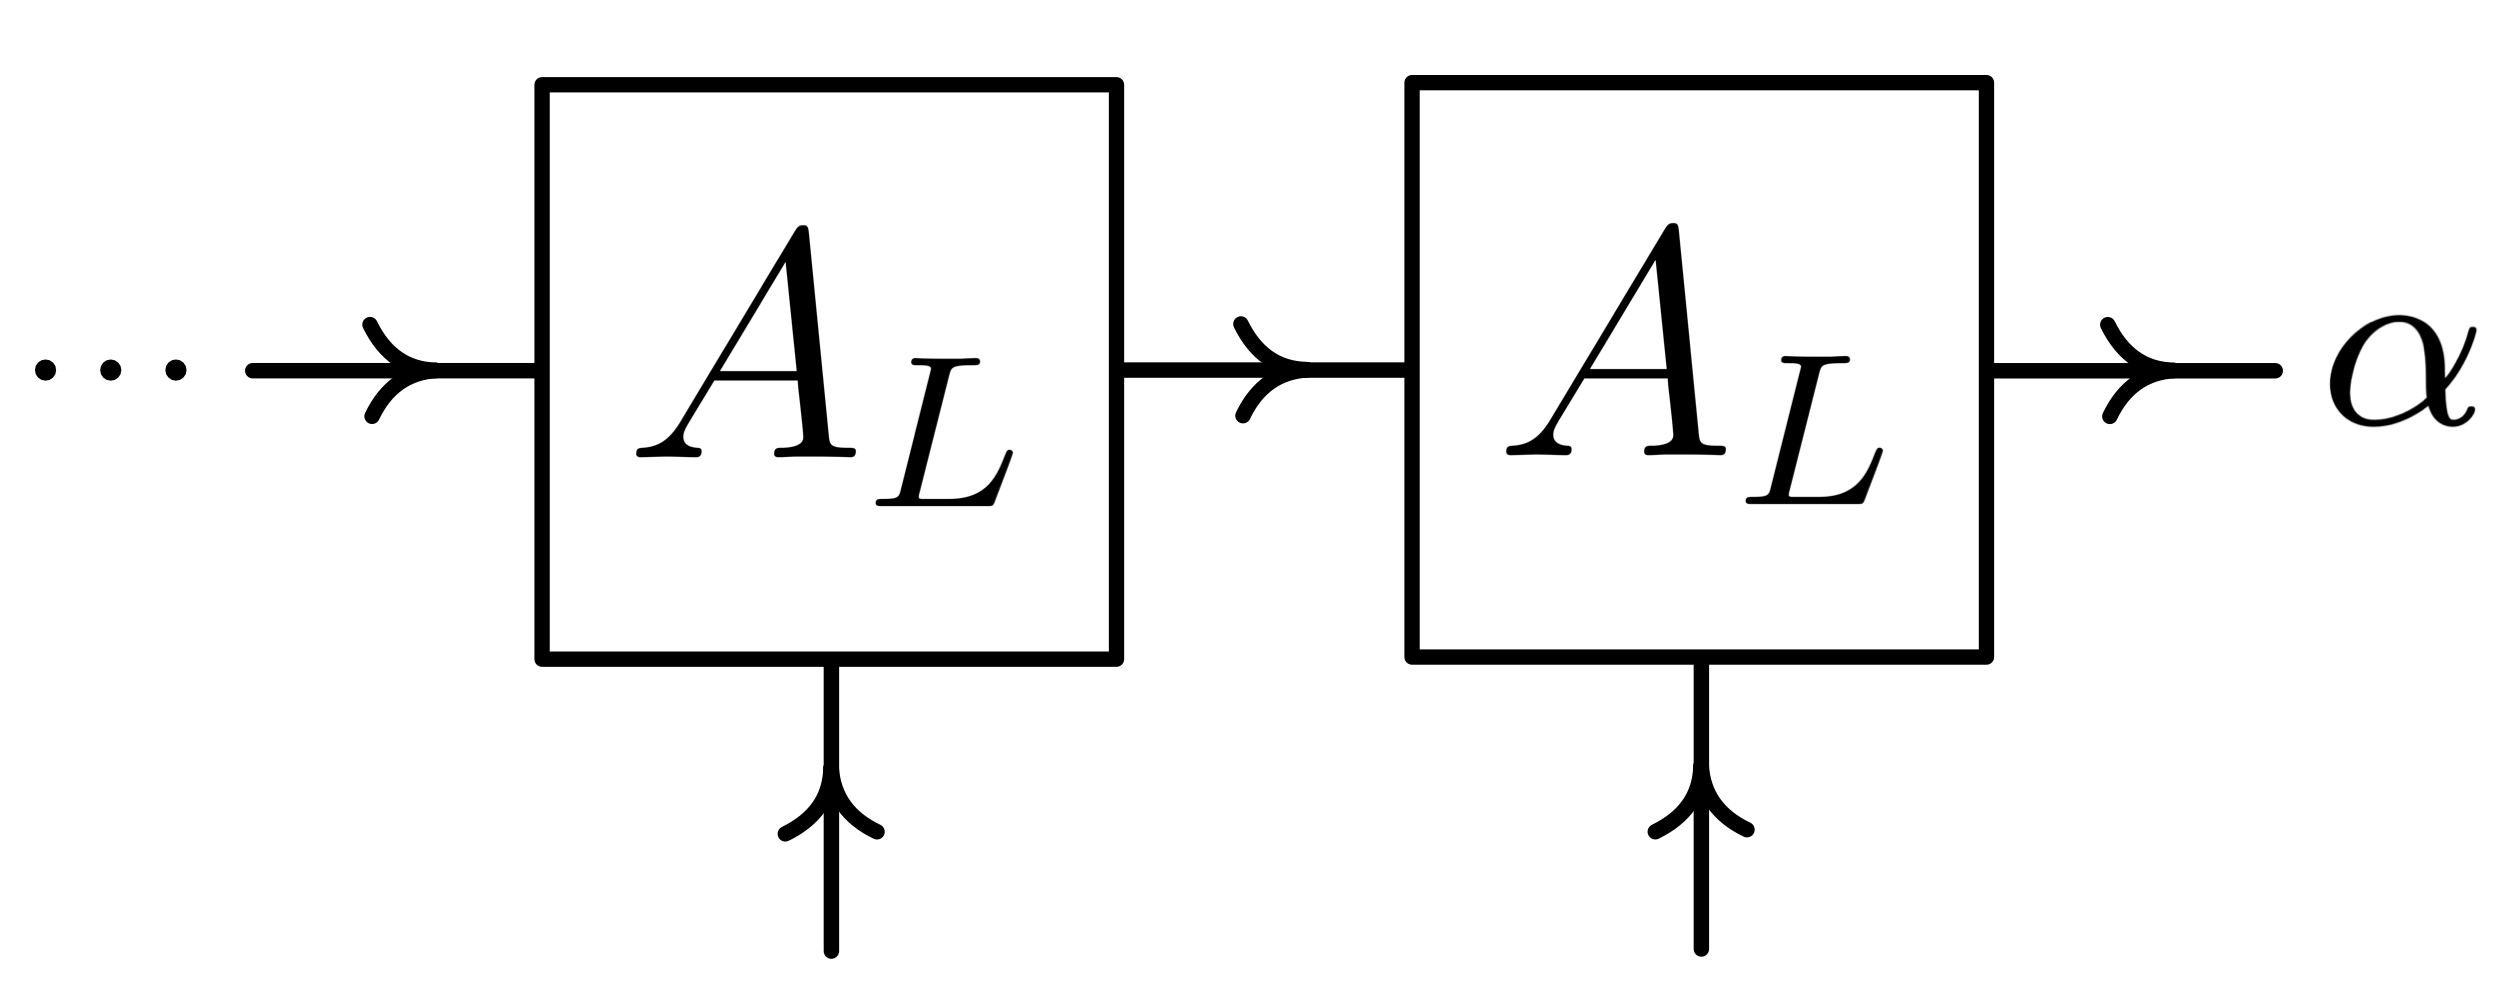
\includegraphics[height=1.3cm]{psi_AL.png}}, \:\: \ket{\psi(A_R)_{\alpha}} = \raisebox{-0.55\height}{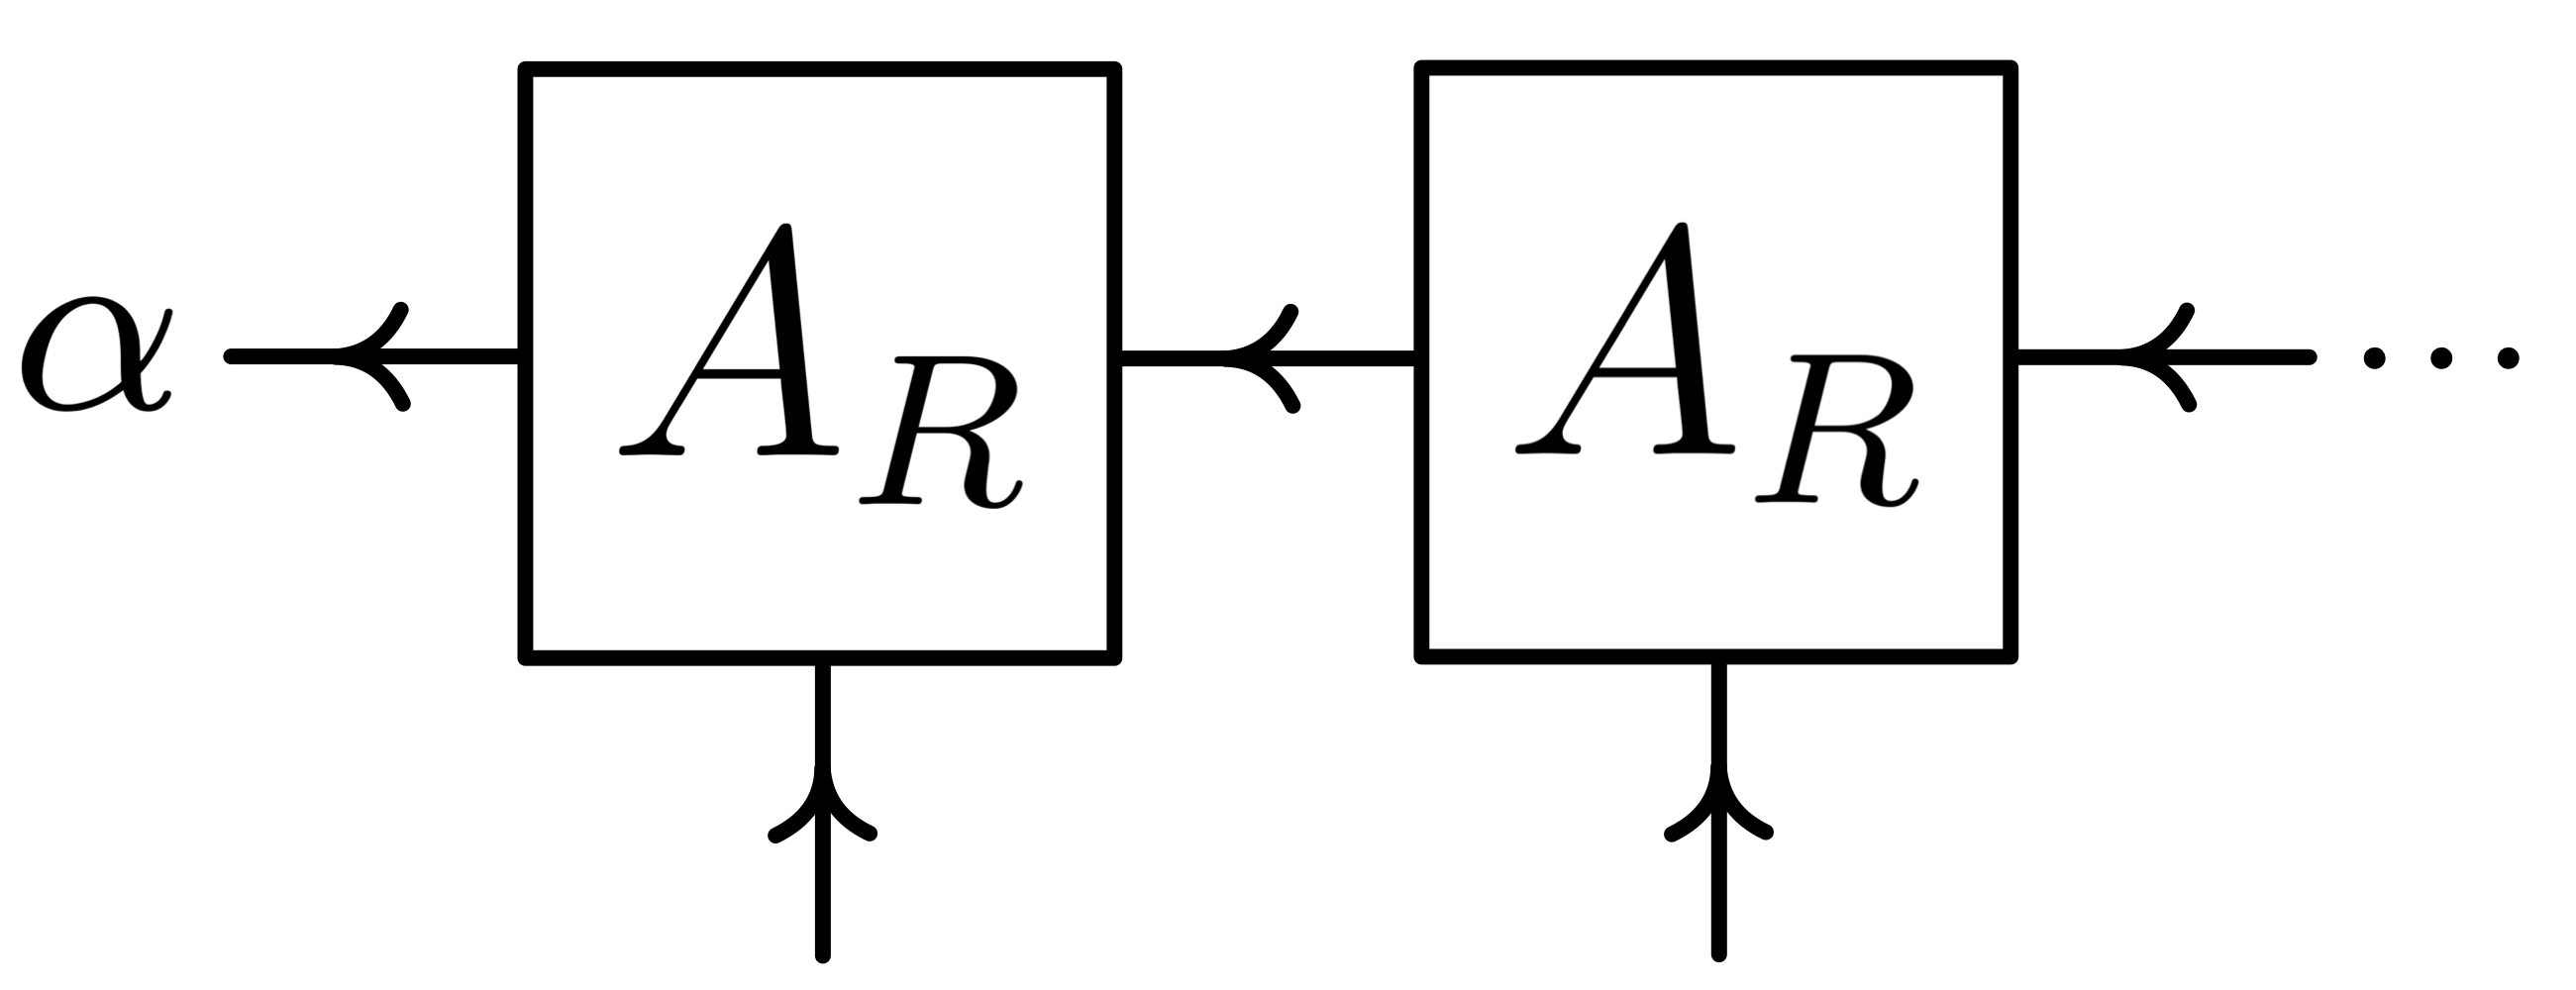
\includegraphics[height=1.3cm]{psi_AR.png}}
\end{equation}
are orthonormal, i.e. $\langle \psi (\overline{A}_L)_{\alpha} \vert \psi (A_L)_{\beta} \rangle = \delta_{\alpha \beta}$, $\langle \psi (\overline{A}_R)_{\alpha} \vert \psi (A_R)_{\beta} \rangle = \delta_{\alpha \beta}$, this is nothing but a \textit{Schmidt decomposition} with \textit{Schmidt values} $C_{\alpha} > 0$ and \textit{Schmidt rank} $D$.
From this, the reduced density matrix $\rho_L = \mathrm{tr}_R \ket{\psi (A)}\bra{\psi (\overline{A})}$ yields the \textit{entanglement entropy}
\begin{equation}
	S({\psi_A}) = - \mathrm{tr}[\rho_L \log \rho_L] = - \sum_{\alpha = 1}^D C_{\alpha}^2 \log C_{\alpha}^2.
\end{equation}
This shows that the bond dimension $D$ controls the amount of entanglement in the uMPS. More precisely, it sets an upper bound for the bipartite entanglement entropy:
\begin{equation} \label{eq:umps_entanglement}
	S({\psi_A}) \leq \log D.
\end{equation}
As we know, the full Hilbert space is exponentially large in the chain length $N$, and \cite{page1993average} proved that a typical random state fulfills a \textit{volume law} for the entanglement entropy:
\begin{equation} 
	S(\psi_{\mathrm{random}}) \approx \frac{N}{2} \log d - \frac{1}{2},
\end{equation}
scaling extensively with the subsystem size $N/2$. The good news is that ground states of local, gapped Hamiltonians are very special and lie in a small corner of the Hilbert space. Proven by \cite{hastings2007area} and strengthened by \cite{arad2013area}, the entanglement entropy of these ground states scales with the area of the boundary between the two subsystems, which is a constant in one spatial dimension. This is called the \textit{area law}:
\begin{equation} \label{eq:area_law}
	S(\psi_0) \leq \mathcal{O}[(\log d)^3 / \Delta],
\end{equation}
where $\Delta$ denotes the energy gap above the ground state. The bounds \eqref{eq:umps_entanglement} and \eqref{eq:area_law} indicate: Ground states of local, gapped Hamiltonians can be faithfully approximated by uMPS with bond dimension $D = \mathcal{O}(e^{(\log d)^3 / \Delta})$. \\[0.5em]
\noindent Conversely, in appendix \ref{ch:quantum_channels_mps}, we prove that for any $\ket{\psi (A)} \in \mathcal{M}_D$, we can define a local, \textit{frustration free}\footnote{In the sense that the ground state minimizes the energy locally for each term in the Hamiltonian.} Hamiltonian, of which $\ket{\psi (A)}$ is the exact, unique ground state. This Hamiltonian is called \textit{parent Hamiltonian} and it can be shown to be gapped.


% VUMPS
\section{Variational uniform matrix product states (VUMPS)} \label{sec:vumps}
\noindent We now present a variational algorithm \cite{zauner2018variational} that minimizes the energy of a local Hamiltonian $H$ within the manifold $\mathcal{M}_D$ of uniform matrix product states:
\begin{equation}
	\argmin_{A \in \mathcal{A}_D} \frac{\bra{\psi(\overline{A})} H \ket{\psi(A)}}{\langle \psi(\overline{A}) \vert \psi(A) \rangle}.
\end{equation}
We can rewrite the stationary condition \eqref{eq:stationary_condition} as
\begin{equation} \label{eq:residual_schrödinger}
	\partial_{\overline{A}} \bra{\psi(\overline{A})} (H - \lambda) \ket{\psi(A)} = 0.
\end{equation}
For a variational optimum $\ket{\psi(A)}$ with energy $\lambda =  \bra{\psi(\overline{A})} H \ket{\psi(A)}$, \eqref{eq:residual_schrödinger} forces the residual $(H - \lambda) \ket{\psi(A)}$ of the full Schrödinger equation---which is not exactly solvable within the manifold---to be orthogonal to the space spanned by the states $\partial_A \ket{\psi(A)}$, which is equal to the tangent space $\mathcal{T}_{\ket{\psi (A)}}$. Denoting with $P_{\mathcal{T}_{\ket{\psi (A)}}}$ the projector onto the tangent space at point $\ket{\psi(A)}$, \eqref{eq:residual_schrödinger} can be reformulated as the projective Schrödinger equation
\begin{equation} \label{eq:projective_schrödinger}
	P_{\mathcal{T}_{\ket{\psi (A)}}} (H - \lambda) \ket{\psi(A)} = 0.
\end{equation}

% projector
\noindent \underline{Projector onto tangent space} \\[0.5em]
\noindent We derive a diagrammatic expression for $P_{\mathcal{T}_{\ket{\psi (A)}}}$. We do this in the canonical gauge \eqref{eq:umps_canonical_form}. Our starting point is a tangent space vector $\ket{\psi(B; A)}$ in the left gauge, so equal to \eqref{eq:tangent_space_vector} but with $A_L$ instead of $A$. For each state in the superposition, we then bring all tensors on the right of site $n$ into right isometric form. The remaining full rank matrix $C$ can be absorbed into the (unnormalized) perturbation tensor $B$ and we end up with
\begin{equation} \label{eq:tangent_space_vector_canonical}
	\ket{\psi (B; A)} = \sum_n \raisebox{-0.47\height}{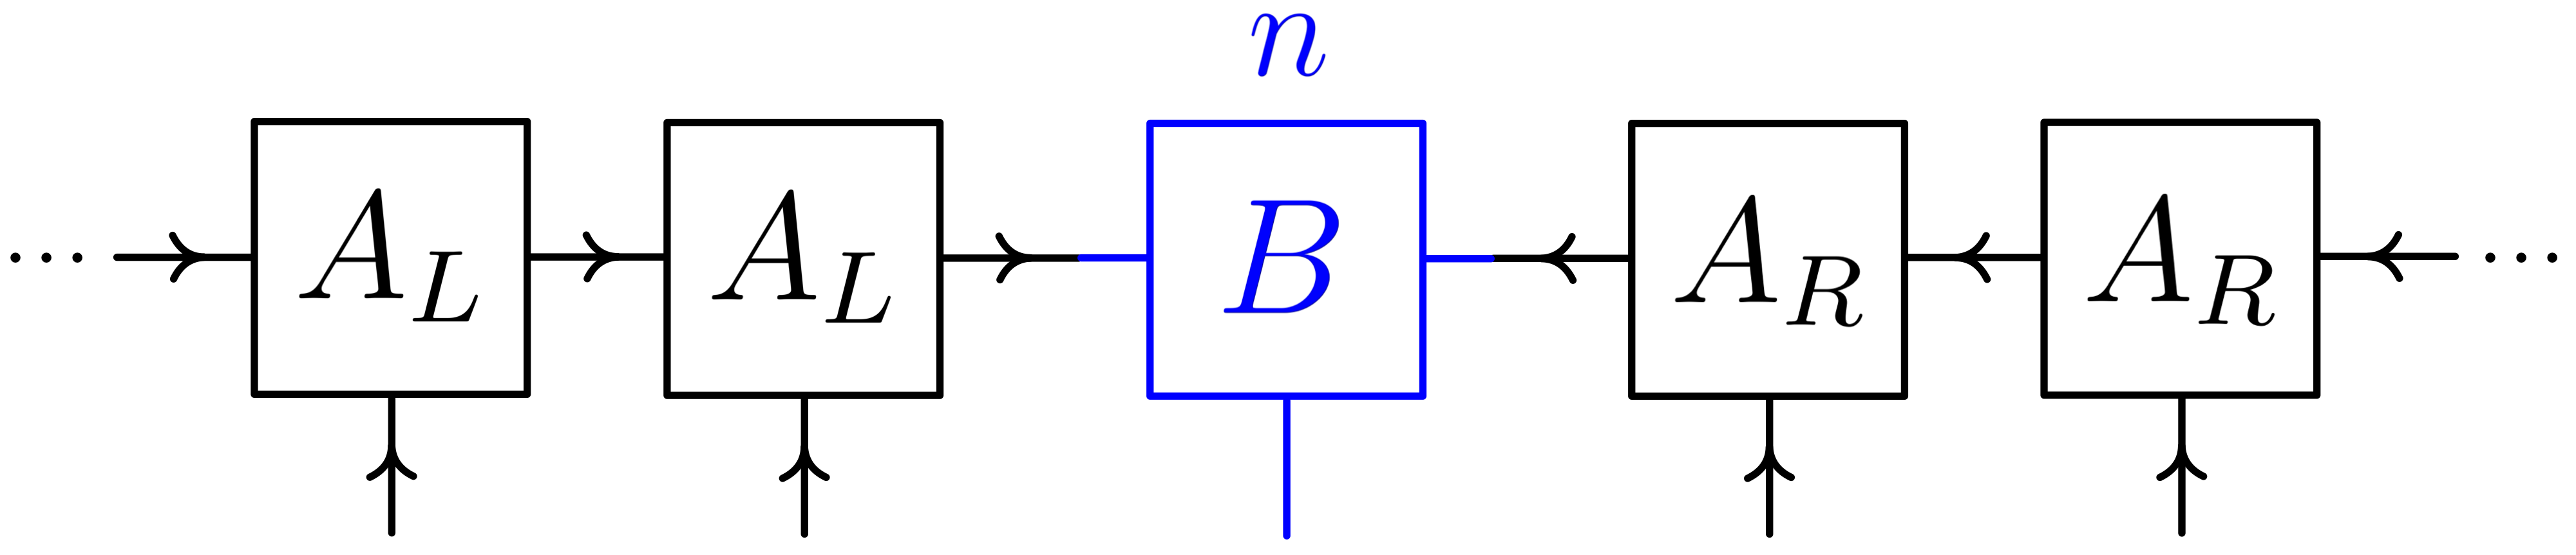
\includegraphics[height=1.4cm]{tangent_vector_canonical.png}} \hspace{0.2em}.
\end{equation}
For any $Y \in \mathbb{C}^{D \times D}$ this state is left invariant under the gauge transformation 
\begin{equation}
	B \rightarrow B + A_L Y - Y A_R.
\end{equation}
We fix the $D^2$ gauge parameters by the effective parametrization
\begin{equation}
	\raisebox{-0.55\height}{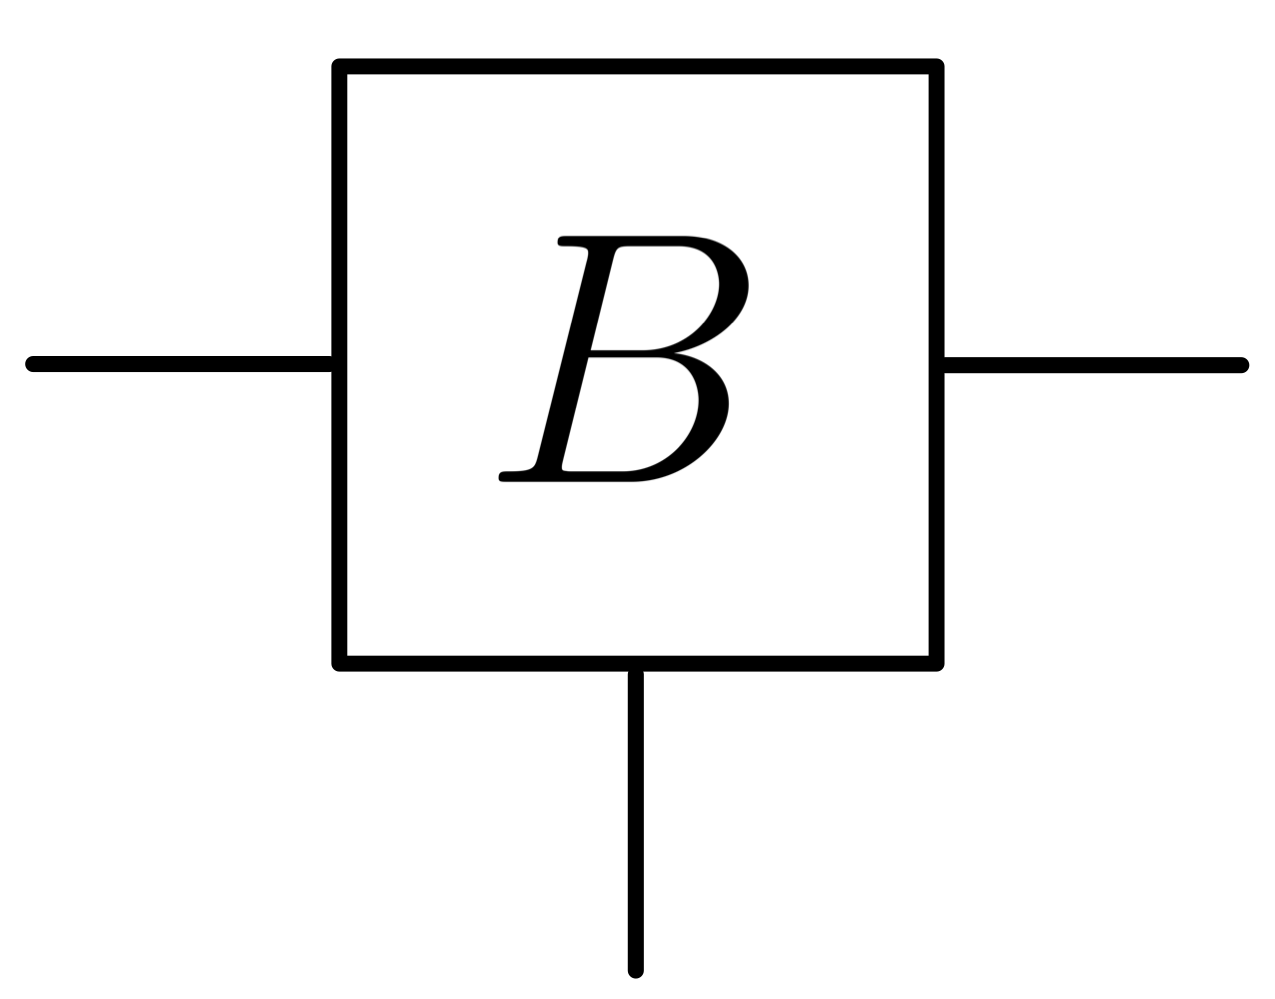
\includegraphics[height=1.2cm]{B.png}} \: = \: \raisebox{-0.55\height}{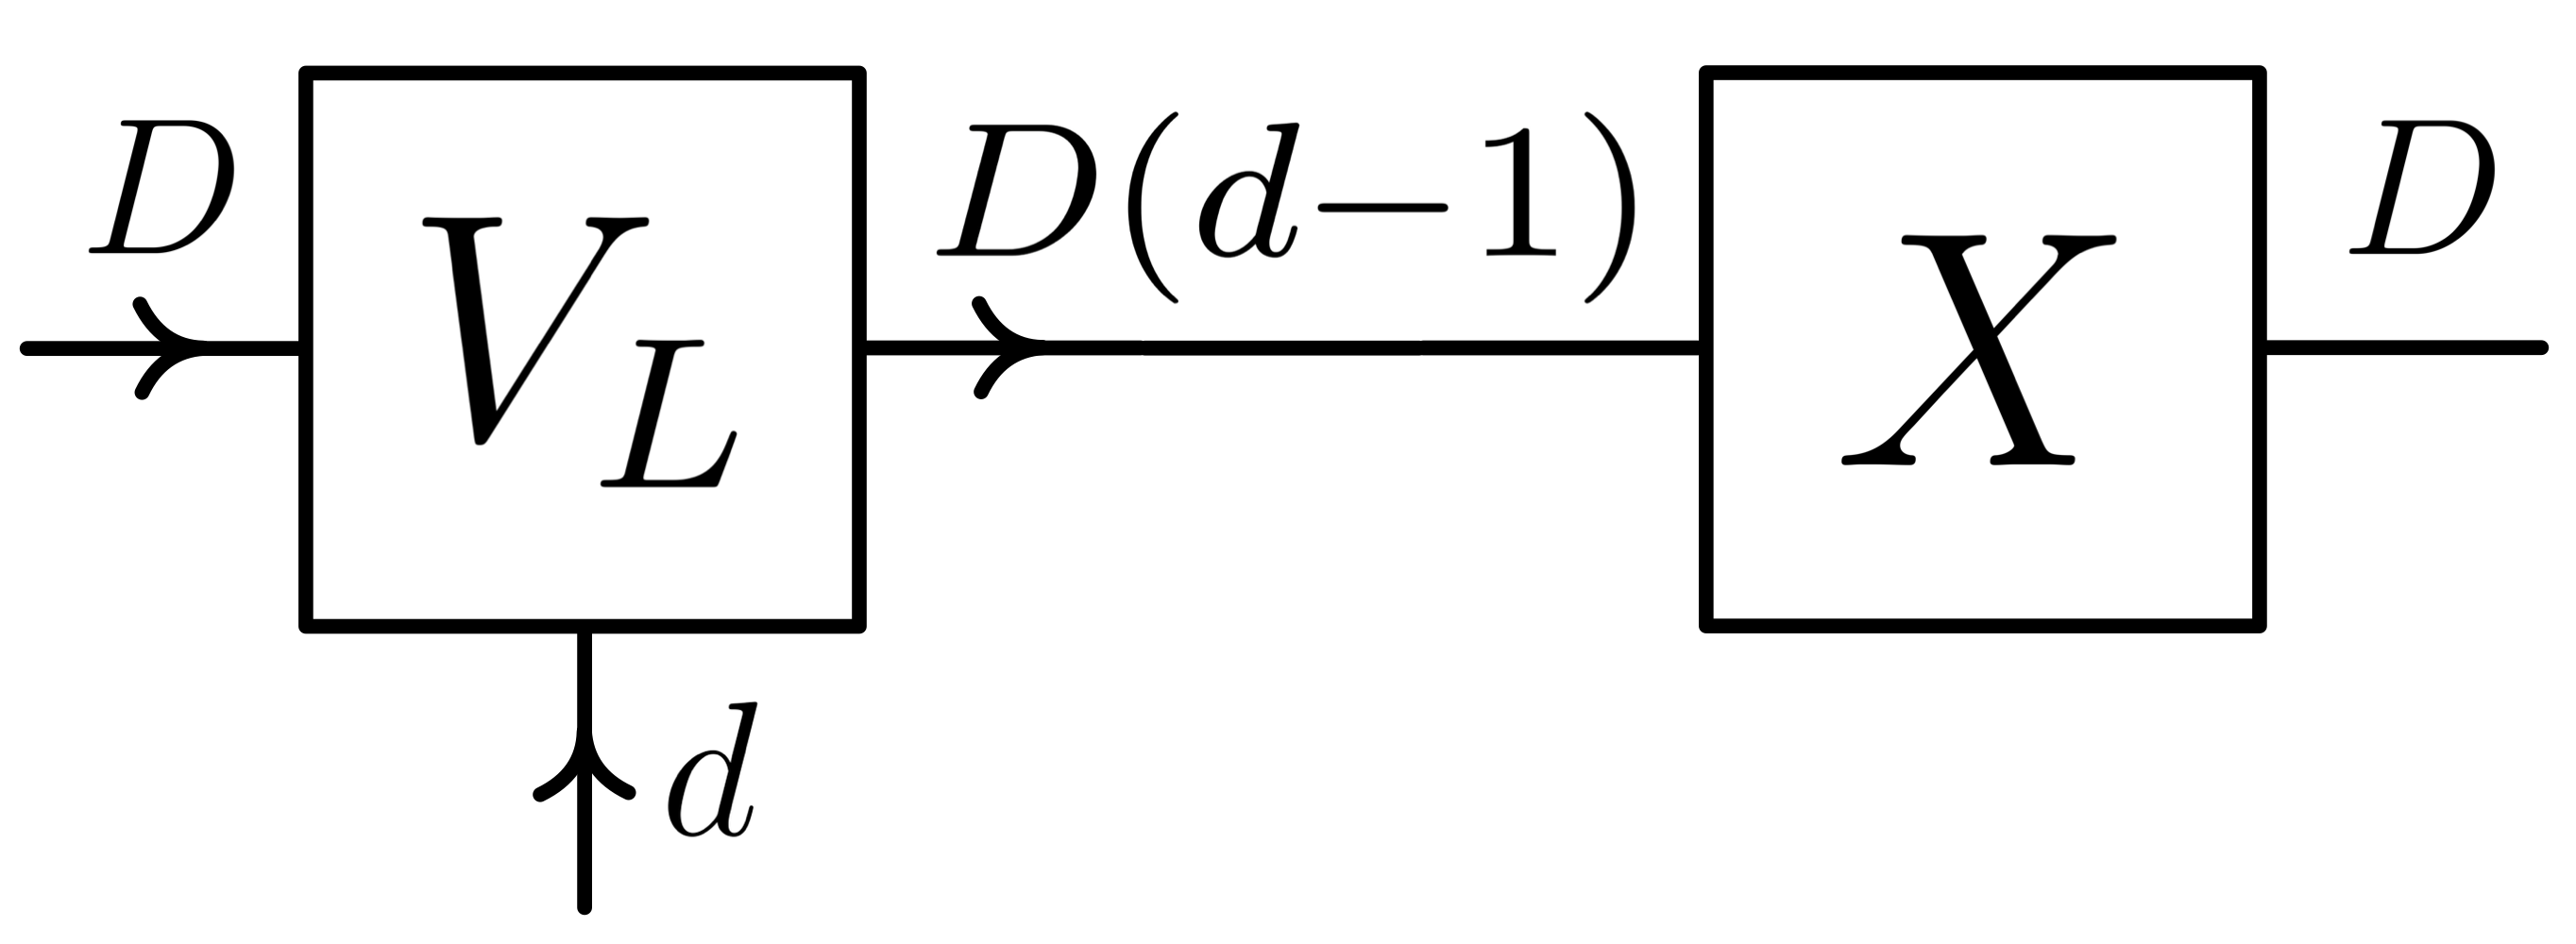
\includegraphics[height=1.2cm]{VL_X.png}} \:\: \text{ with } \:\: \raisebox{-0.45\height}{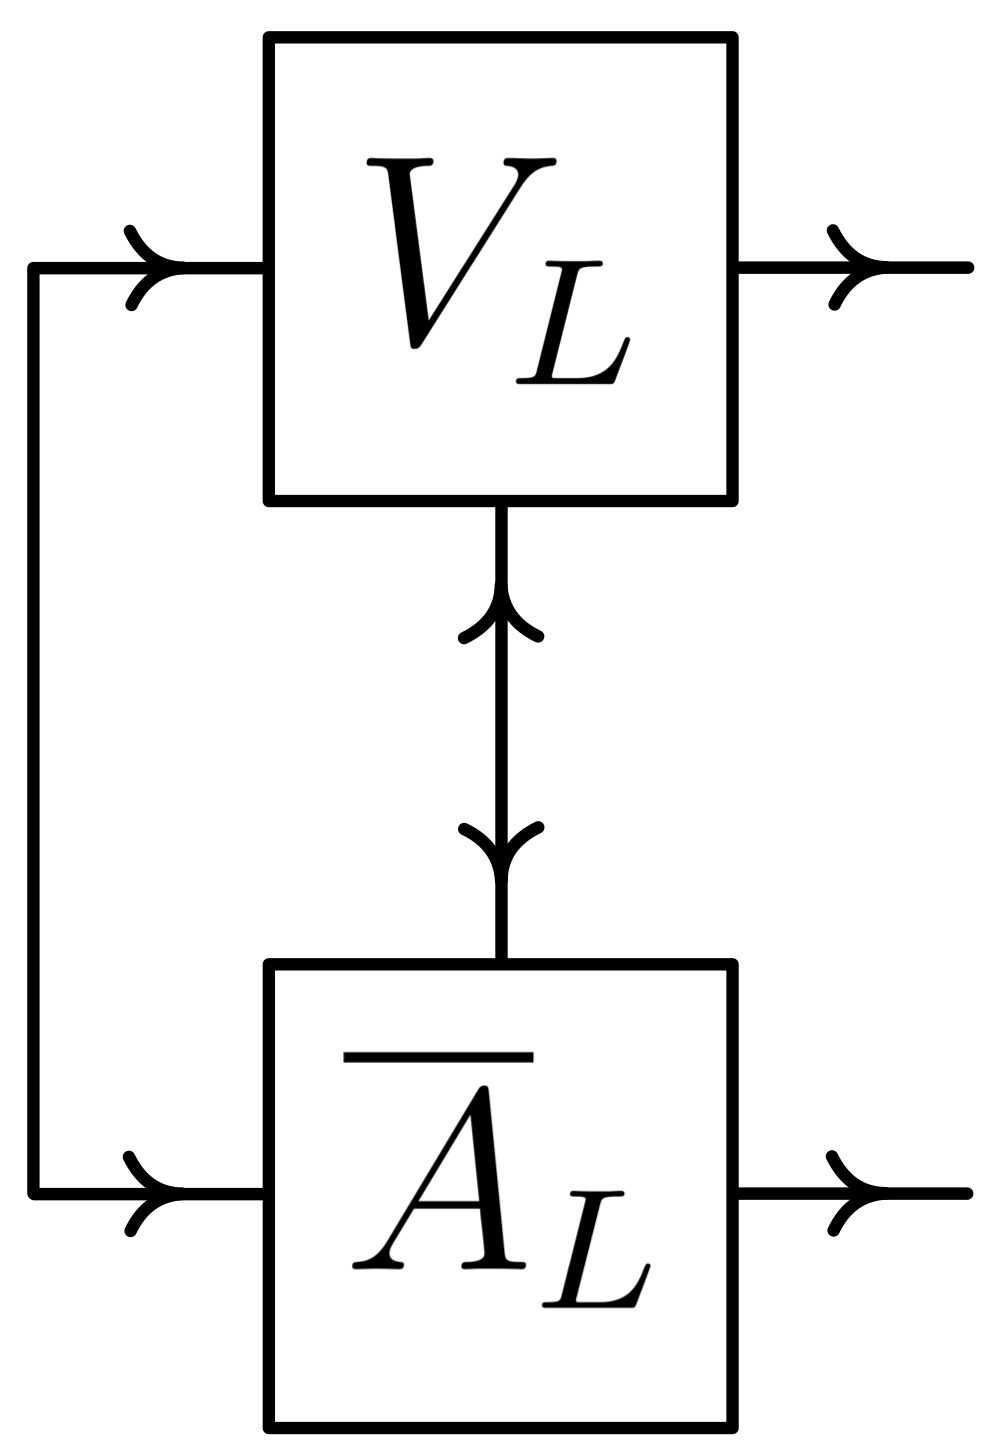
\includegraphics[height=2.2cm]{VL_AL.png}} = 0.
\end{equation}
This not only ensures that the tangent space vectors 
\begin{equation} \label{eq:tangent_space_vector_X}
	\ket{\psi (X; A)} = \sum_n \raisebox{-0.45\height}{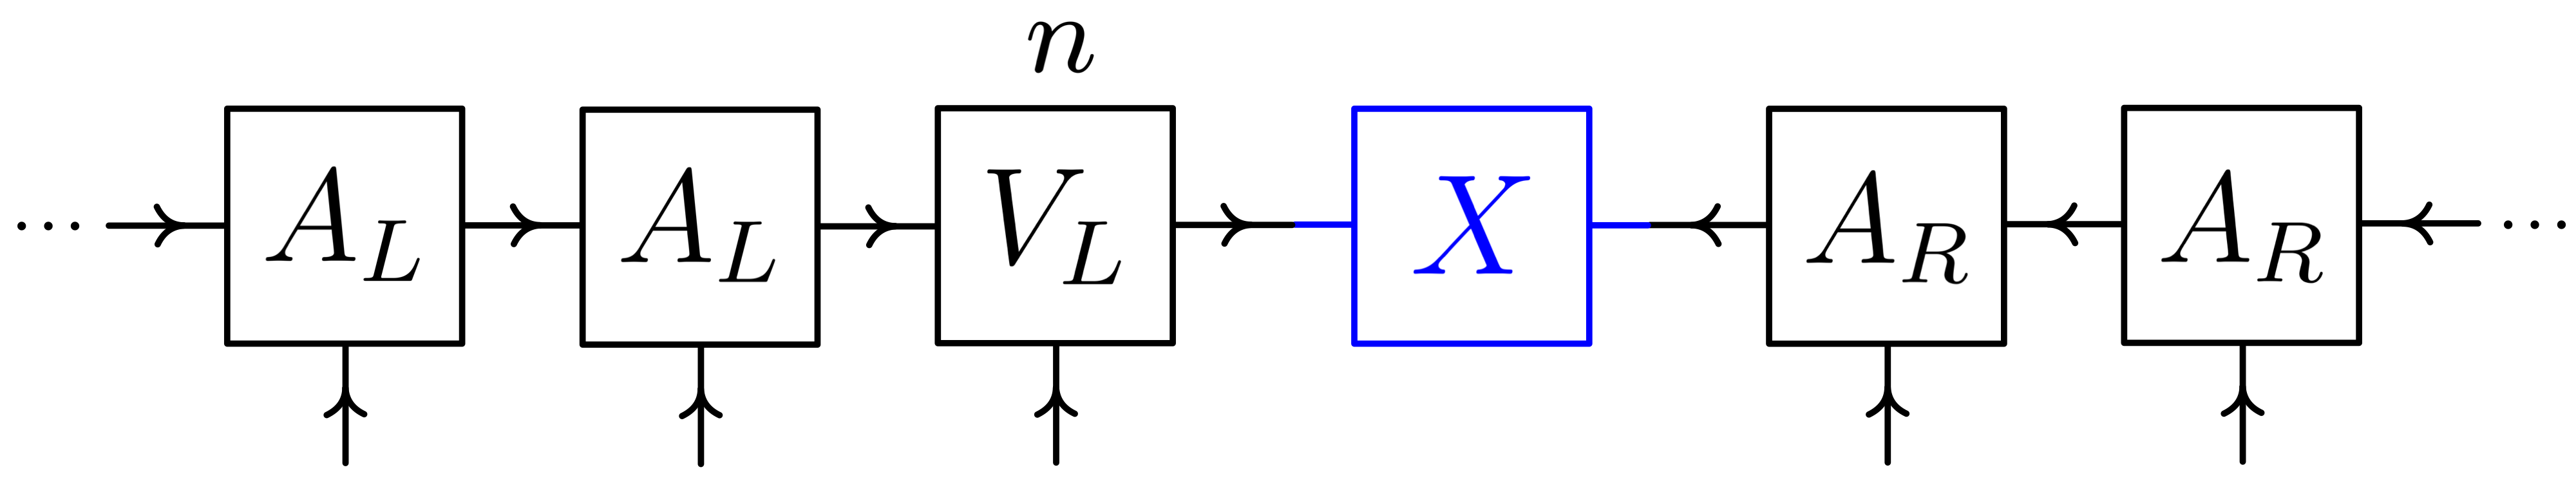
\includegraphics[height=1.45cm]{tangent_vector_X.png}} \hspace{0.5em}
\end{equation}
are orthogonal to the original state $\ket{\psi(A)}$, but also that the overlap between two of them reduces to the overlap between the two parametrizations:
\begin{equation}
	\langle \psi(\overline{Y}; \overline{A}) \vert \psi(X; A) \rangle = \vert \mathbb{Z} \vert ( \overline{Y} \vert X ).
\end{equation}
Finding the projection of an arbitrary translation invariant state in the Hilbert space, $\ket{\varphi} \in \mathcal{H}$, onto the tangent space of $\ket{\psi(A)}$, is equivalent to the following minimization problem:
\begin{align}
\begin{split}
	\min_X \Vert \ket{\varphi} - \ket{\psi(X; A)} \Vert^2 = \min_X \big[ & \langle \psi(\overline{X}; \overline{A}) \vert \psi(X; A) \rangle - \langle \psi(\overline{X}; \overline{A}) \vert \varphi \rangle \\
	& - \langle \varphi \vert \psi(X; A) \rangle + \langle \varphi \vert \varphi \rangle \big].
\end{split}
\end{align}
Setting the derivative of the square bracket with respect to $\overline{X}$ to zero, we get the solution
\begin{equation}
	X_{\varphi} = \partial_{\overline{X}}  \langle \psi(\overline{X}; \overline{A}) \vert \varphi \rangle / \vert \mathbb{Z} \vert.
\end{equation}
The corresponding tangent space vector is
\begin{equation}
	\ket{\psi( X_{\varphi}; A)} = P_{\mathcal{T}_{\ket{\psi (A)}}} \ket{\varphi} = \sum_n \raisebox{-0.4\height}{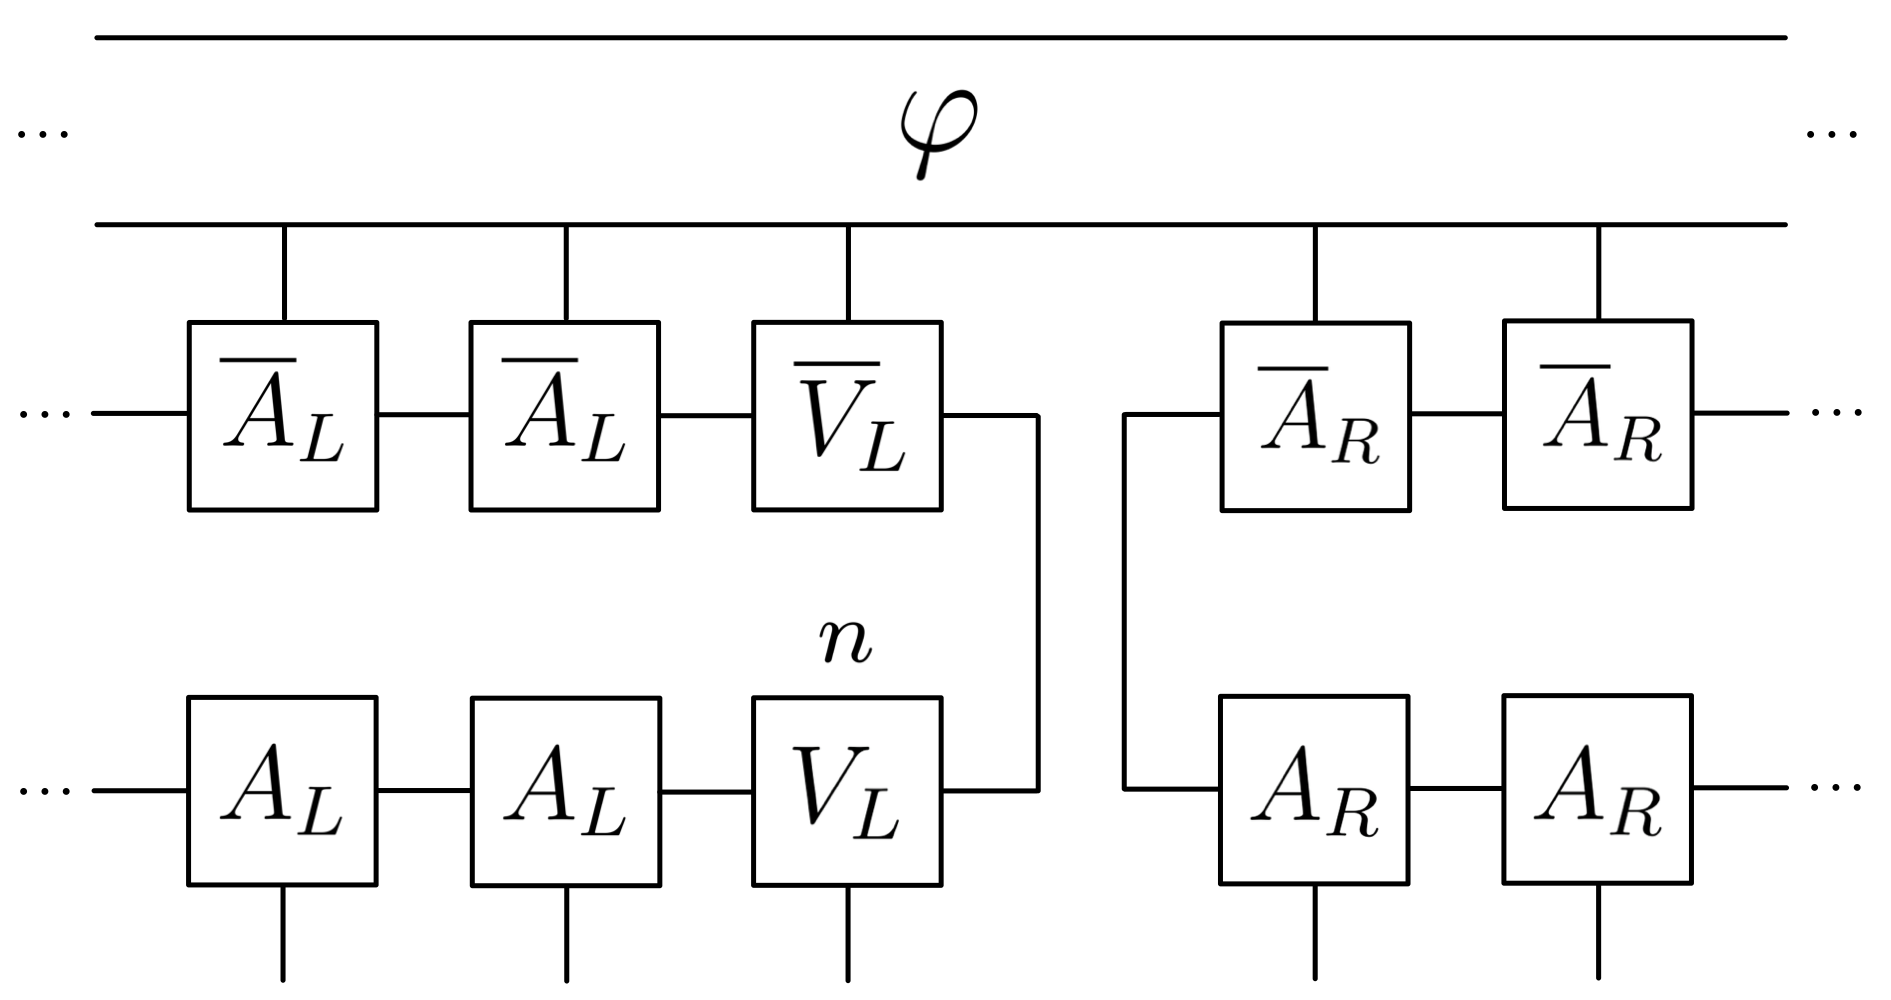
\includegraphics[height=3.7cm]{P_phi.png}} \hspace{0.2em}.
\end{equation}
The columns of the matricized $A_L \in \mathbb{C}^{Dd \times D}$ and $V_L \in \mathbb{C}^{Dd \times D(d-1)}$ together form a unitary matrix. This allows us to insert 
\begin{equation}
	\raisebox{-0.45\height}{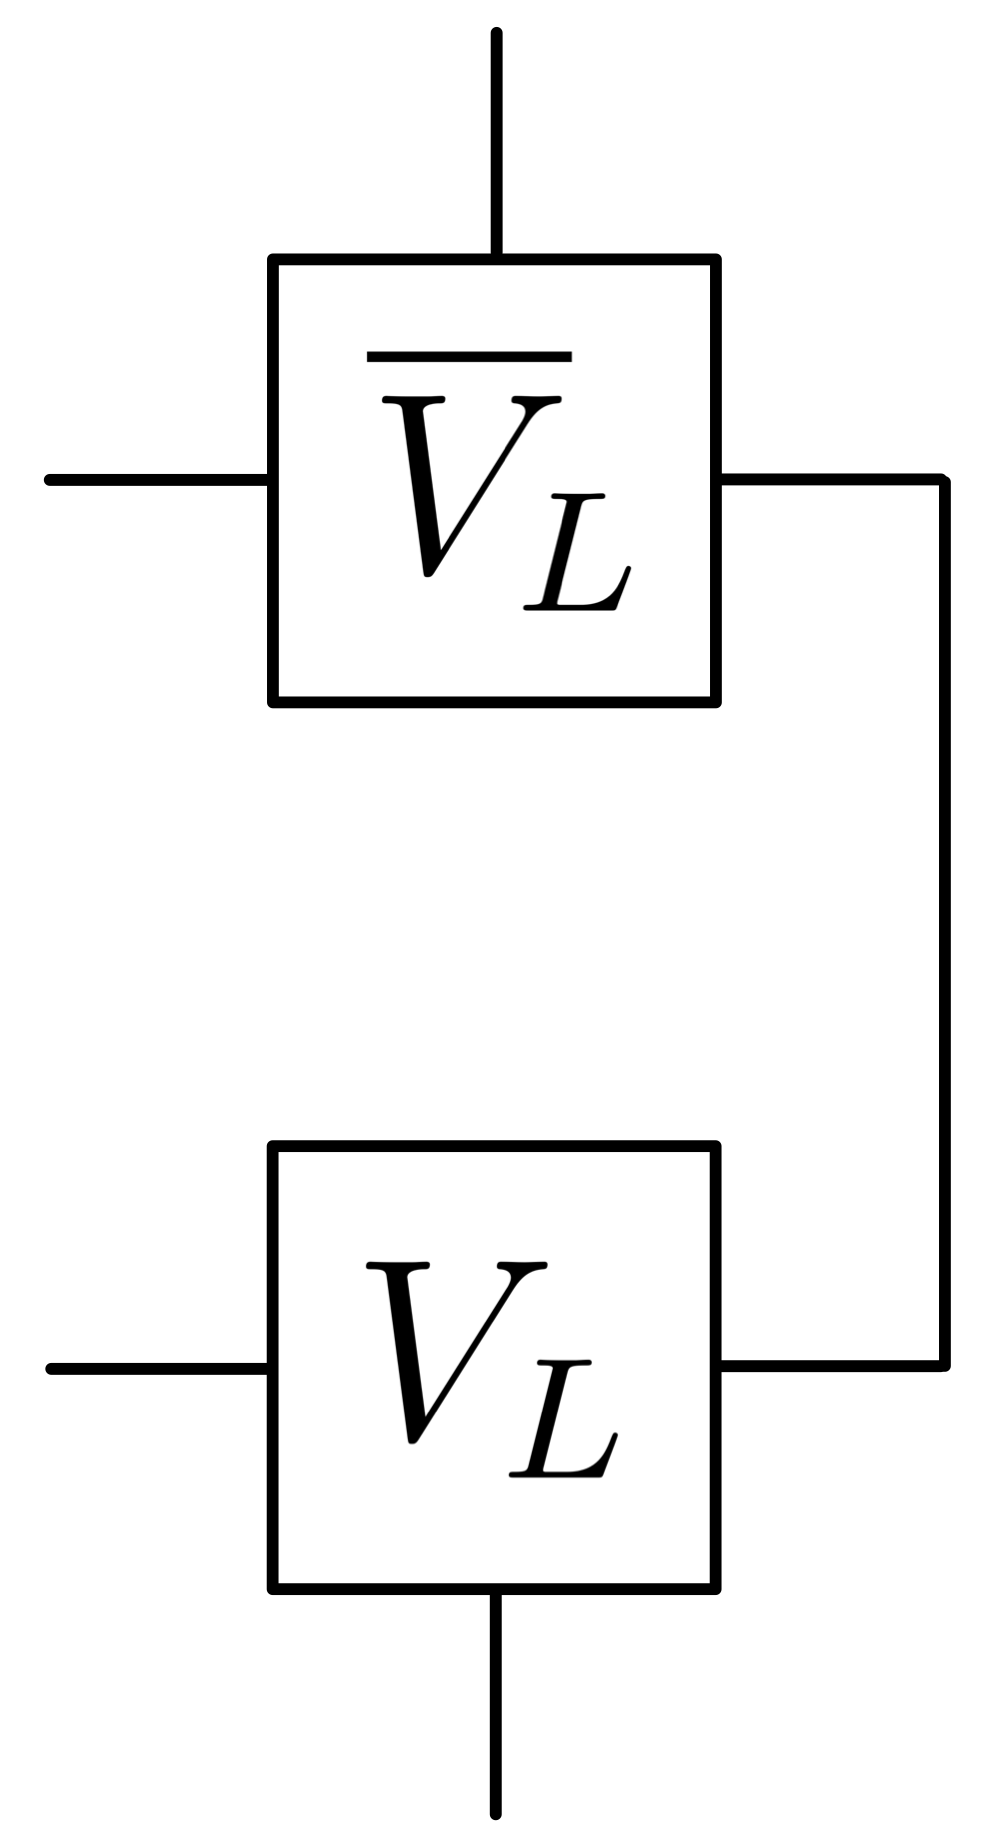
\includegraphics[height=3cm]{VL_VL.png}} \hspace{0.5em} = \raisebox{-0.45\height}{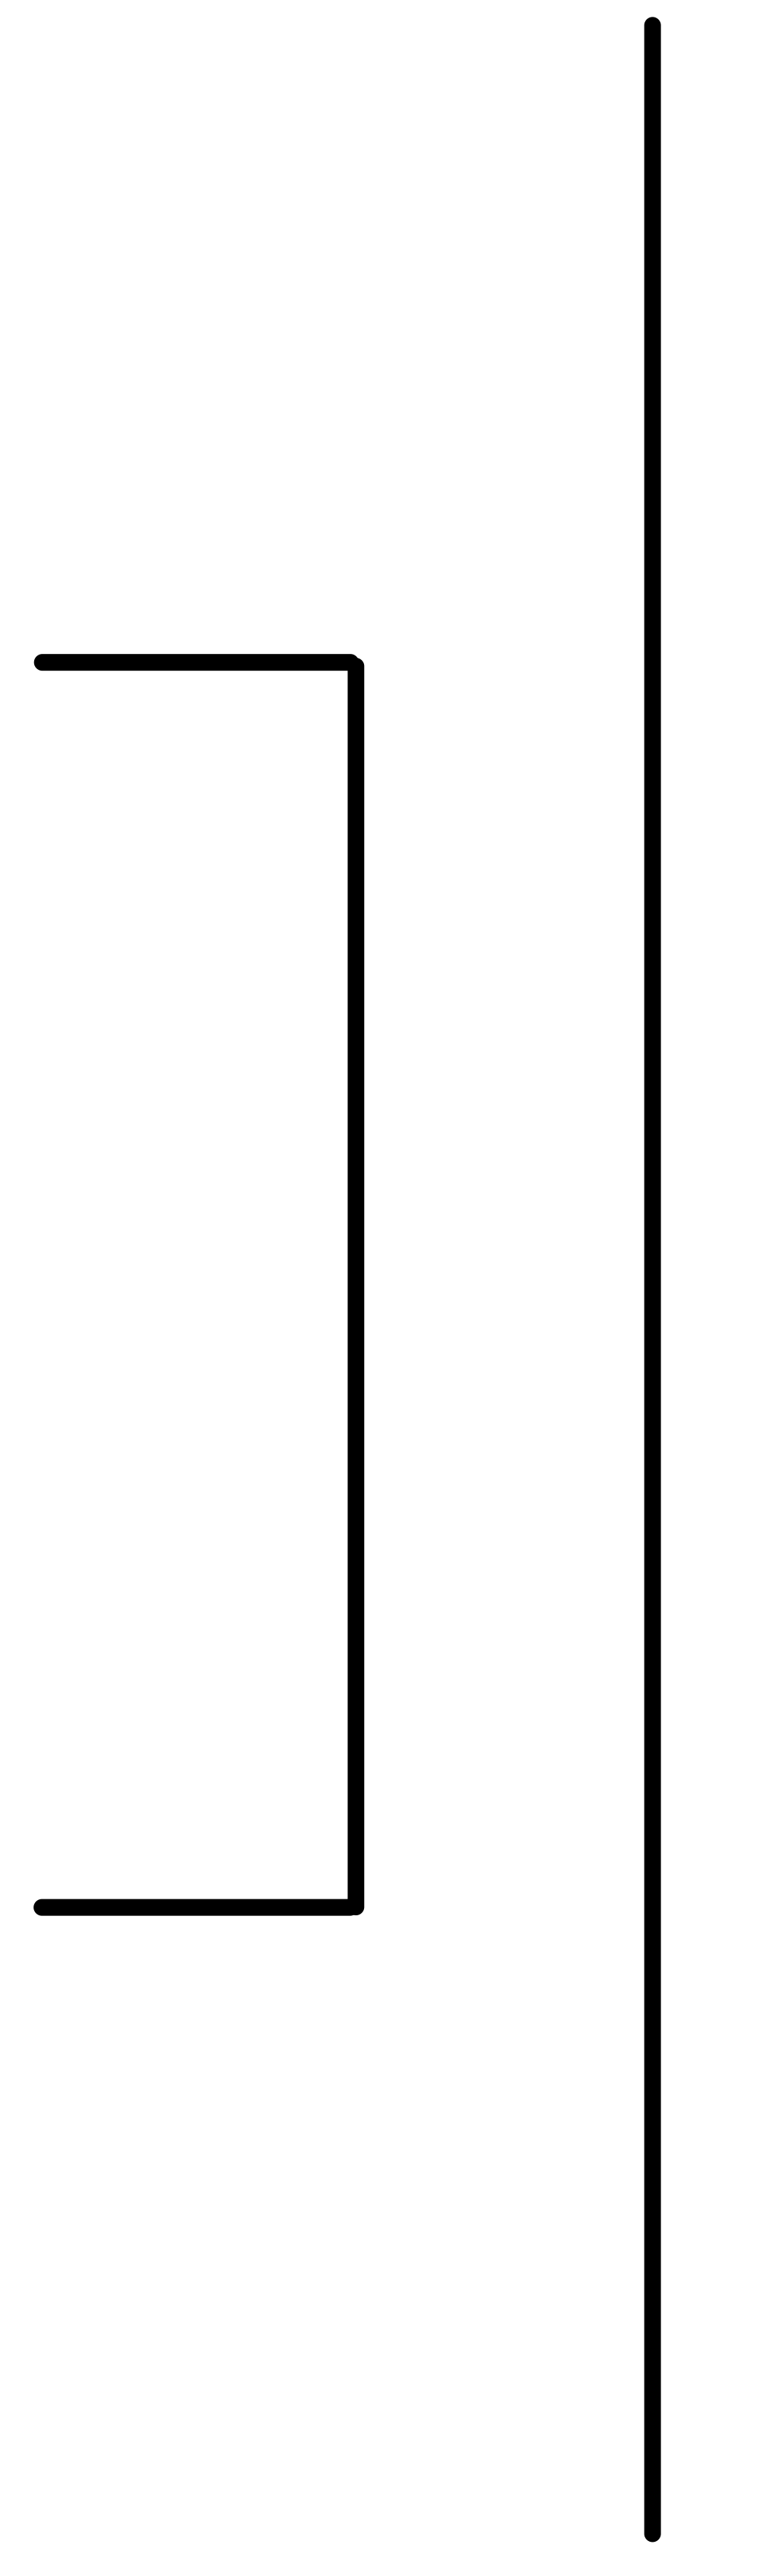
\includegraphics[height=3cm]{Id.png}} \hspace{0.5em} - \raisebox{-0.45\height}{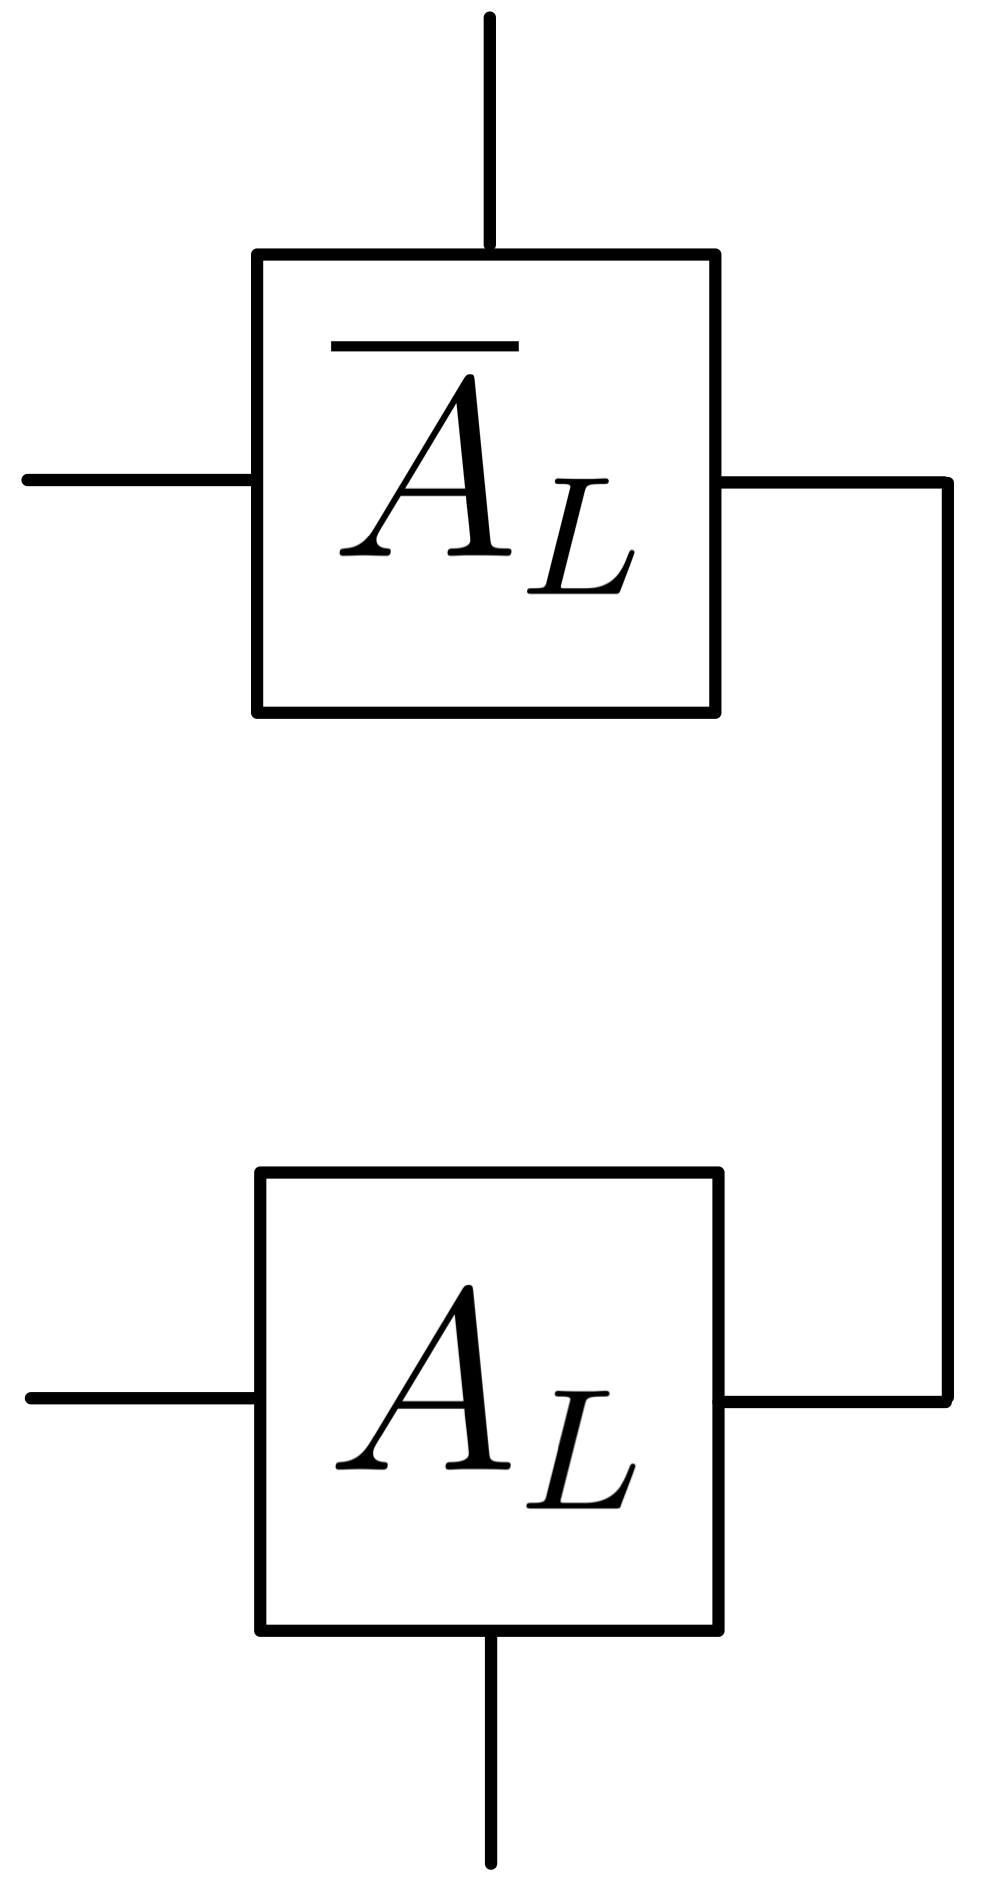
\includegraphics[height=3cm]{AL_AL.png}} \hspace{0.2em},
\end{equation}
and draw the following final form of the tangent space projector:
\begin{equation} \label{eq:projector_tangent_space}
	P_{\mathcal{T}_{\ket{\psi (A)}}} = \sum_n \raisebox{-0.5\height}{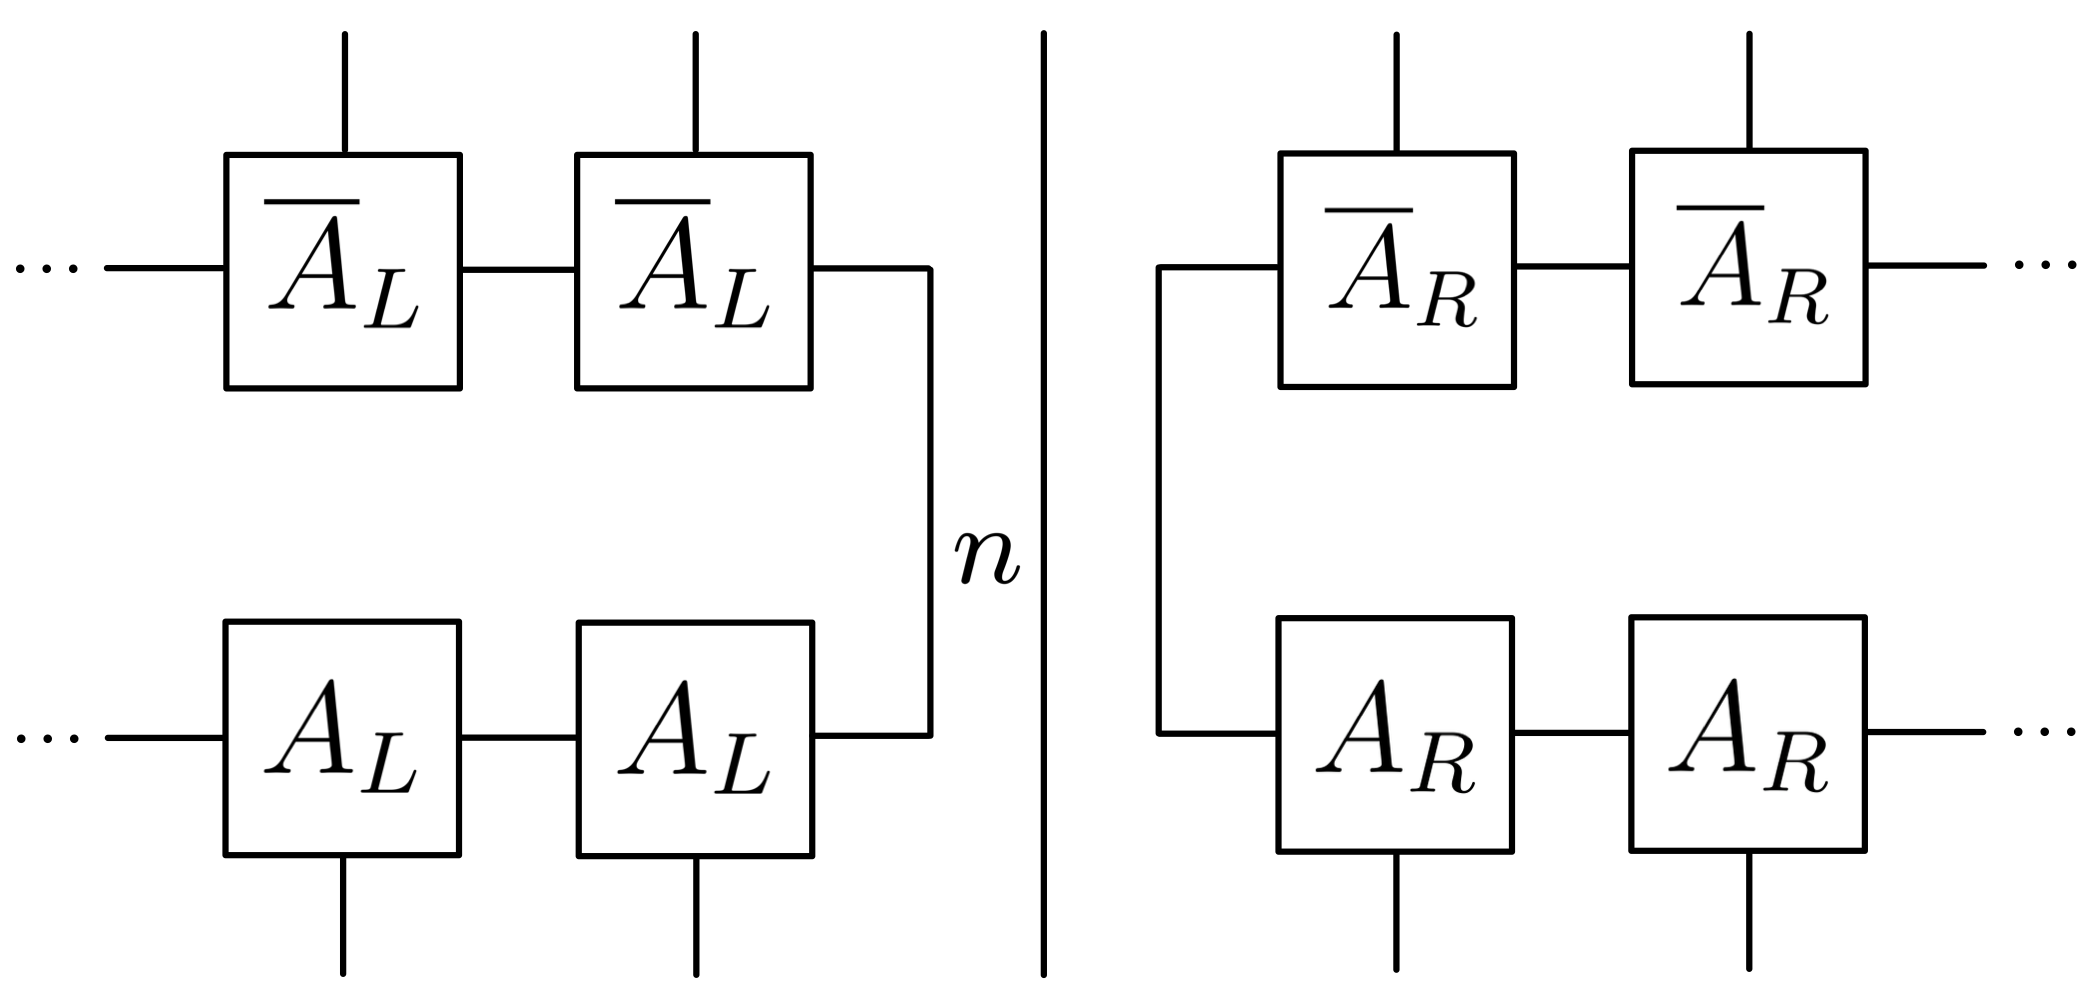
\includegraphics[height=3.0cm]{P1.png}} \hspace{0.5em} 
	 - \sum_n \raisebox{-0.5\height}{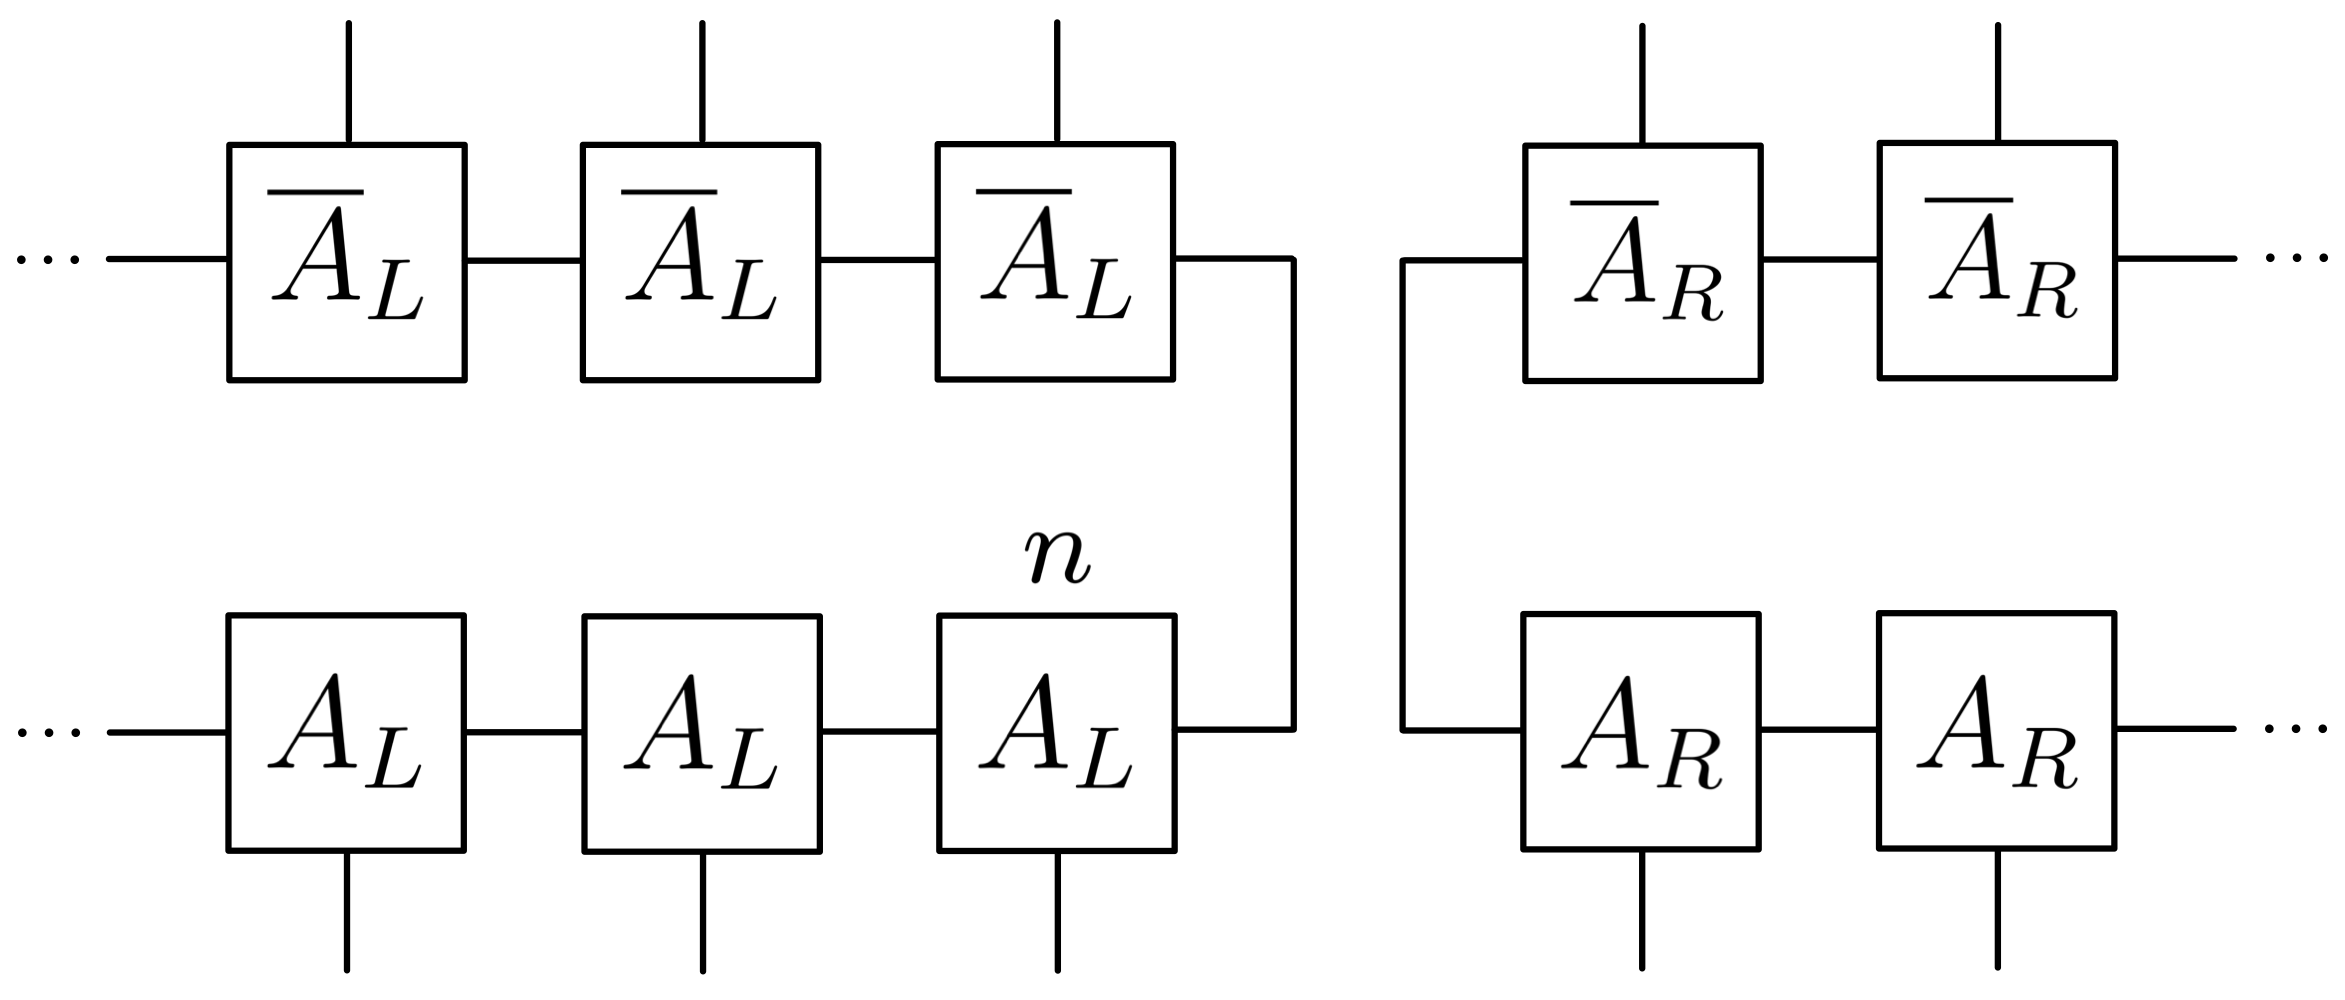
\includegraphics[height=3.0cm]{P2.png}} \hspace{0.2em}.
\end{equation}

% hamiltonian
\noindent \underline{Two-site Hamiltonian} \\[0.5em]
\noindent Describing $d$-dimensional spins on an infinite chain, we assume that $H$ is translational invariant and restricted to nearest neighbor interaction:
\begin{equation} \label{eq:hamiltonian}
	H = \sum_{n \in \mathbb{Z}} h^{[n, n+1]} \:\: \text{ with } h^{[n, n+1]} = \cdots \mathbbm{1} \otimes \mathbbm{1} \otimes \underset{n, \: n+1}{h} \otimes \mathbbm{1} \otimes \mathbbm{1} \cdots, \: h = h^{\dagger} \in \mathbb{C}^{d^2 \times d^2}.
\end{equation}
As an example for $d = 2$, we always have the transverse field Ising model (\ref{eq_ising_hamiltonian_1d}) in mind, with
\begin{equation}
	h = -J (\sigma^x \otimes \sigma^x) - \frac{g}{2} (\sigma^z \otimes \mathbbm{1}) - \frac{g}{2} (\mathbbm{1} \otimes \sigma^z).
\end{equation}
Practically, we store $h$ as a four leg tensor
\begin{equation}
	\raisebox{-0.42\height}{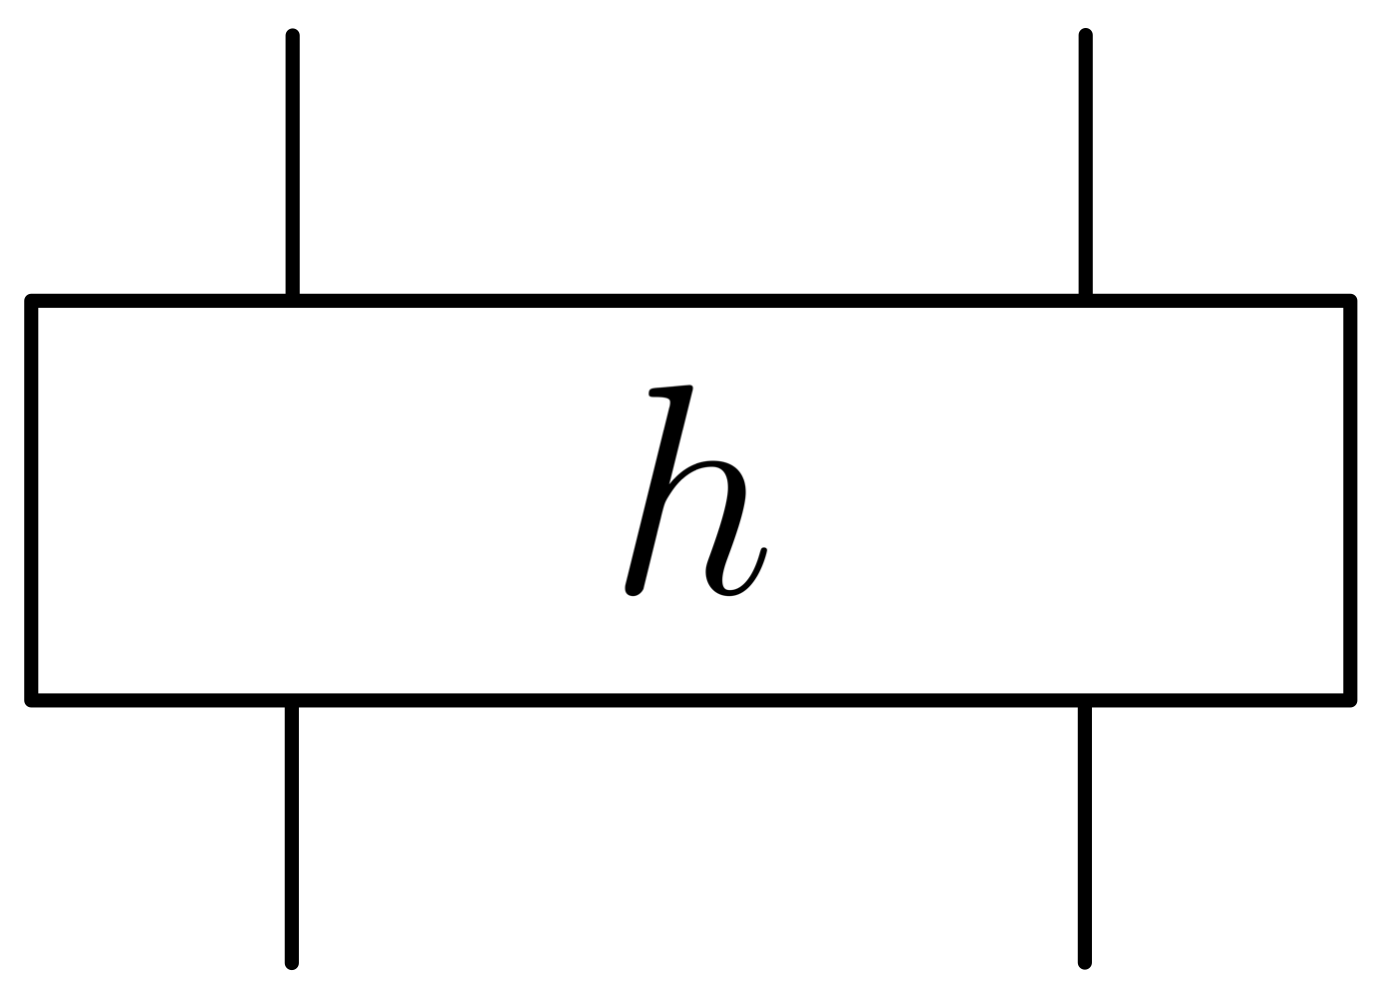
\includegraphics[height=1.5cm]{h.png}} \in \mathbb{C}^{d \times d \times d \times d}.
\end{equation}
Because of translation invariance and the isometric structure of the canonical form, the uMPS expectation value of $H$ reduces to a local energy density $e$ per lattice bond:
\begin{equation}
	\langle \psi(\overline{A}) \vert H \vert \psi(A) \rangle = \vert \mathbb{Z} \vert e \: \text{ with } \: e = \raisebox{-0.48\height}{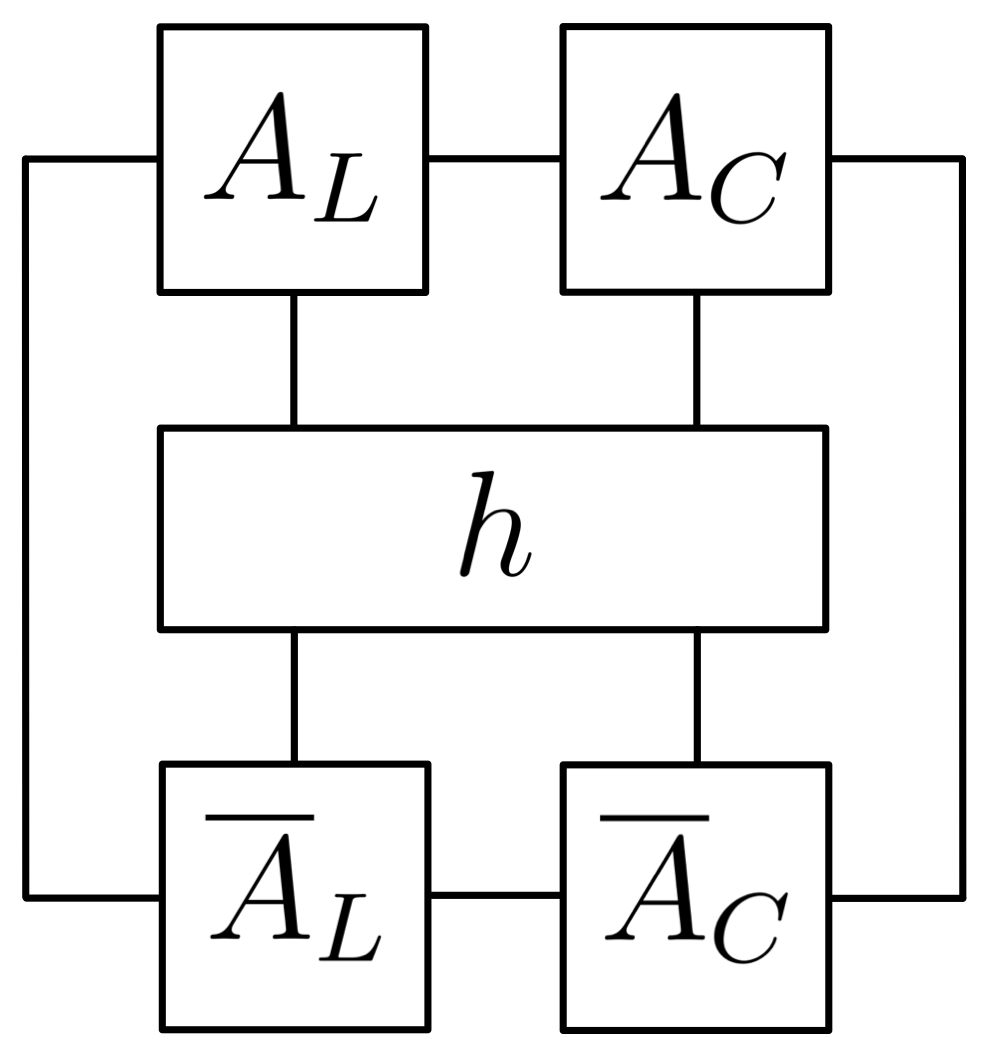
\includegraphics[height=3cm]{e.png}}.
\end{equation}

% vumps
\noindent \underline{VUMPS} \\[0.5em]
We now solve the projected Schrödinger equation \eqref{eq:projective_schrödinger}. Applying the Hamiltonian \eqref{eq:hamiltonian} and then the projector \eqref{eq:projector_tangent_space} to \eqref{eq:umps_canonical_form}, gives the tangent space vector
\begin{equation} \label{eq:projective_schrödinger_applied}
	P_{\mathcal{T}_{\ket{\psi (A)}}} H \ket{\psi (A)} = \ket{\psi (G; A)} \text{ with } G = H_{\mathrm{eff},1}(A_C) - A_L H_{\mathrm{eff},0}(C).
\end{equation}
The effective one site and zero site Hamiltonians act as
\begin{equation}
	\raisebox{-0.5\height}{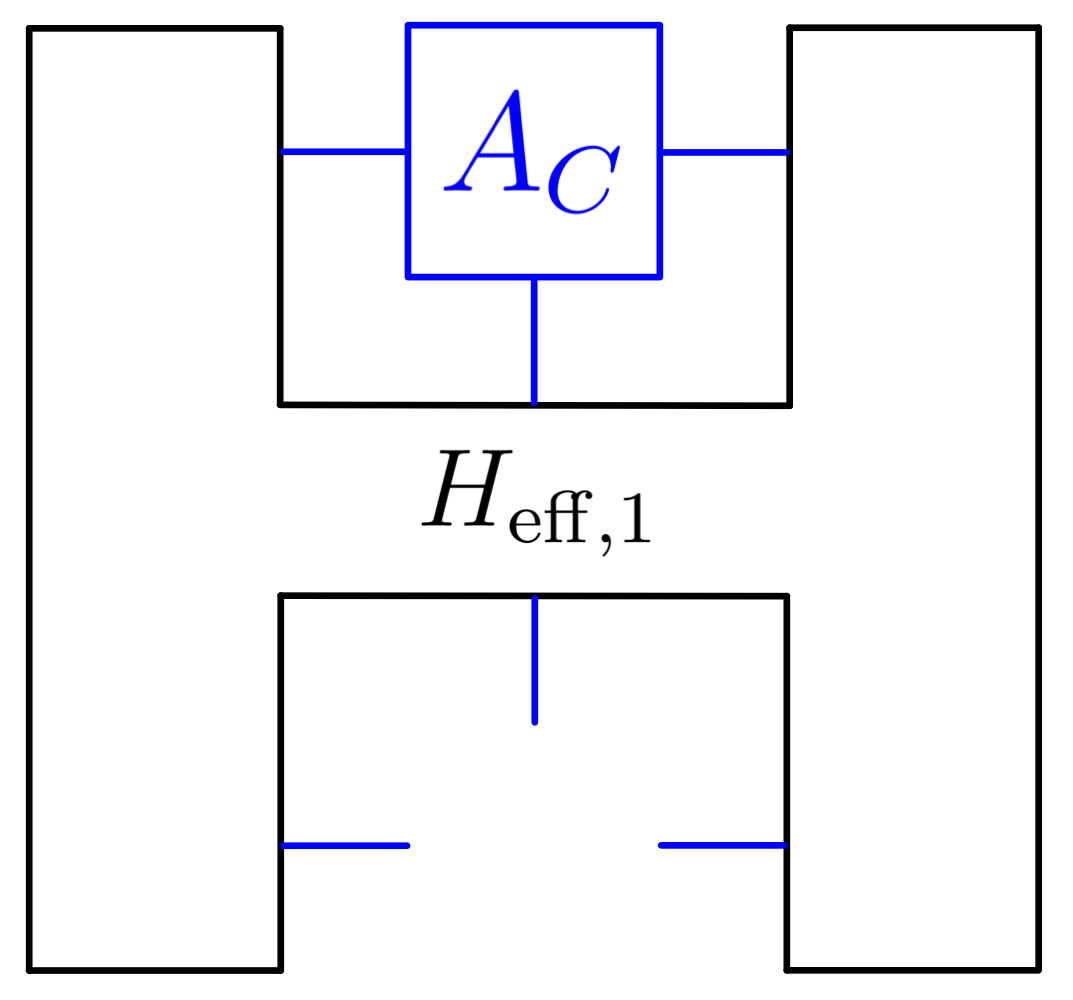
\includegraphics[height=3cm]{Heff1.png}} \: = \: \raisebox{-0.5\height}{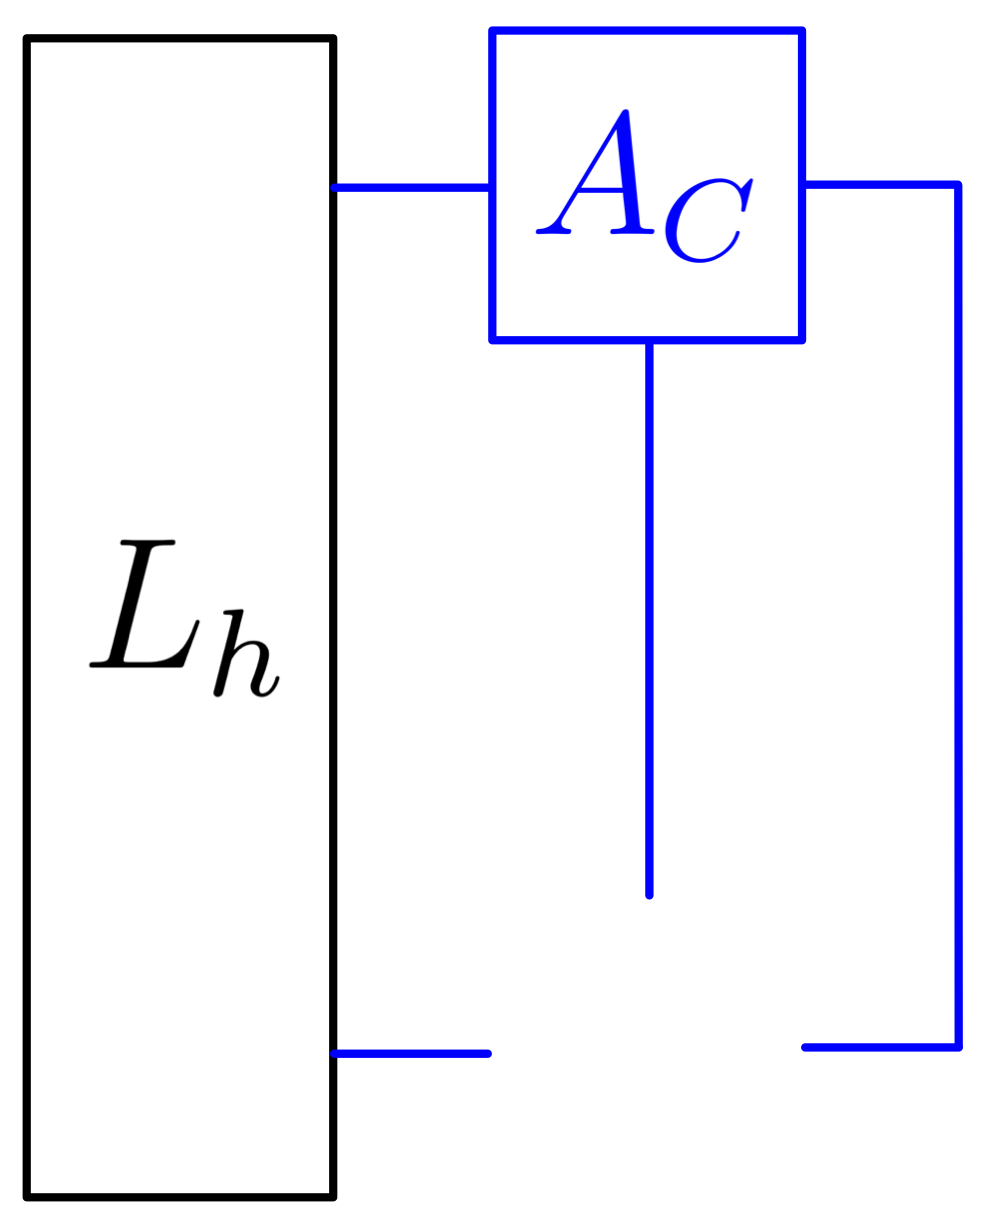
\includegraphics[height=3cm]{Heff1_1.png}} \: + \: \raisebox{-0.5\height}{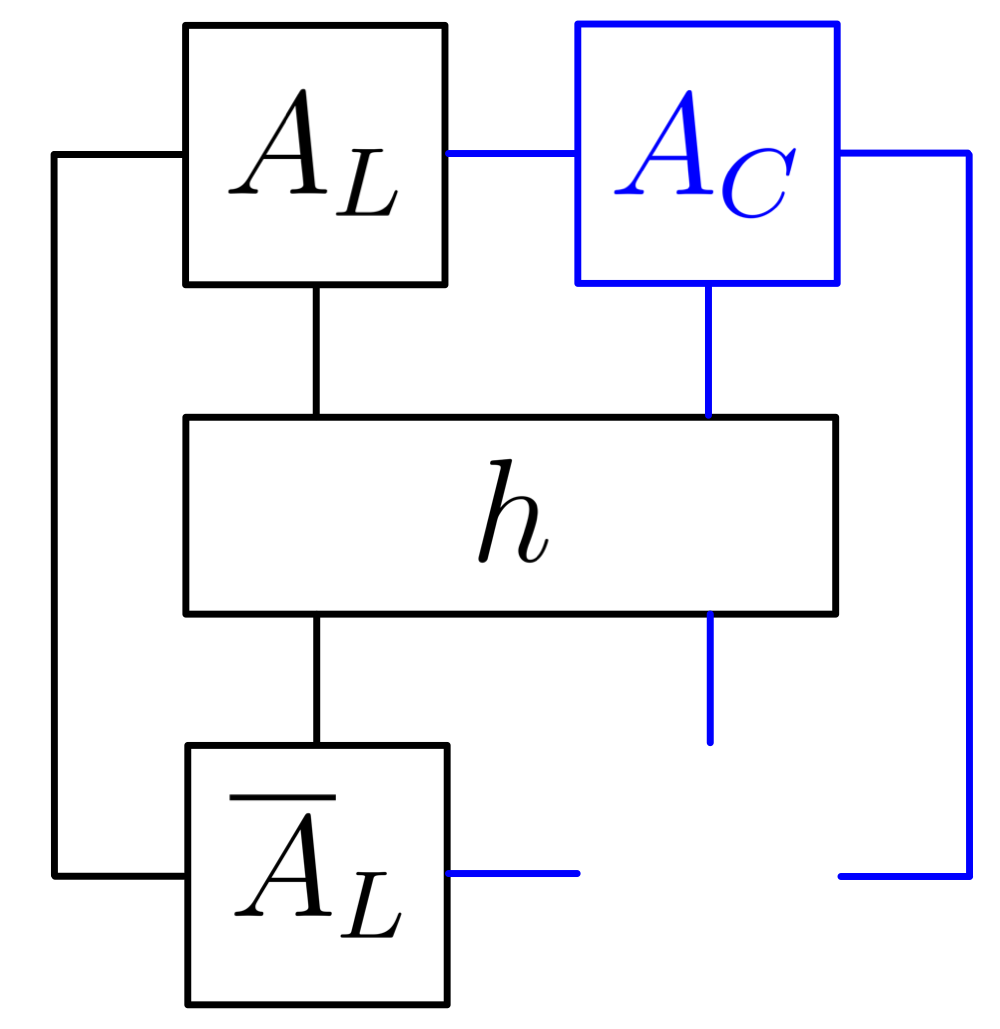
\includegraphics[height=3cm]{Heff1_2.png}} \: + \: \raisebox{-0.5\height}{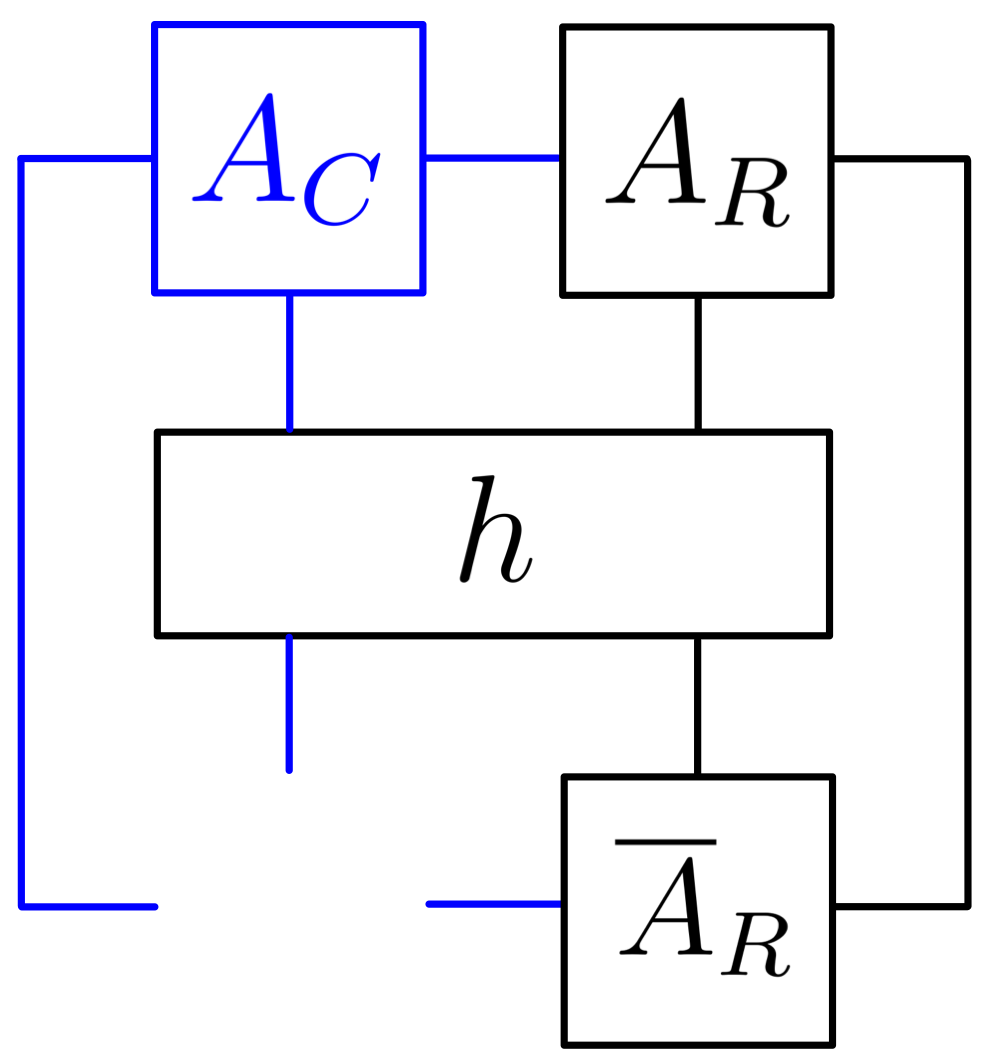
\includegraphics[height=3cm]{Heff1_3.png}} \: + \: \raisebox{-0.5\height}{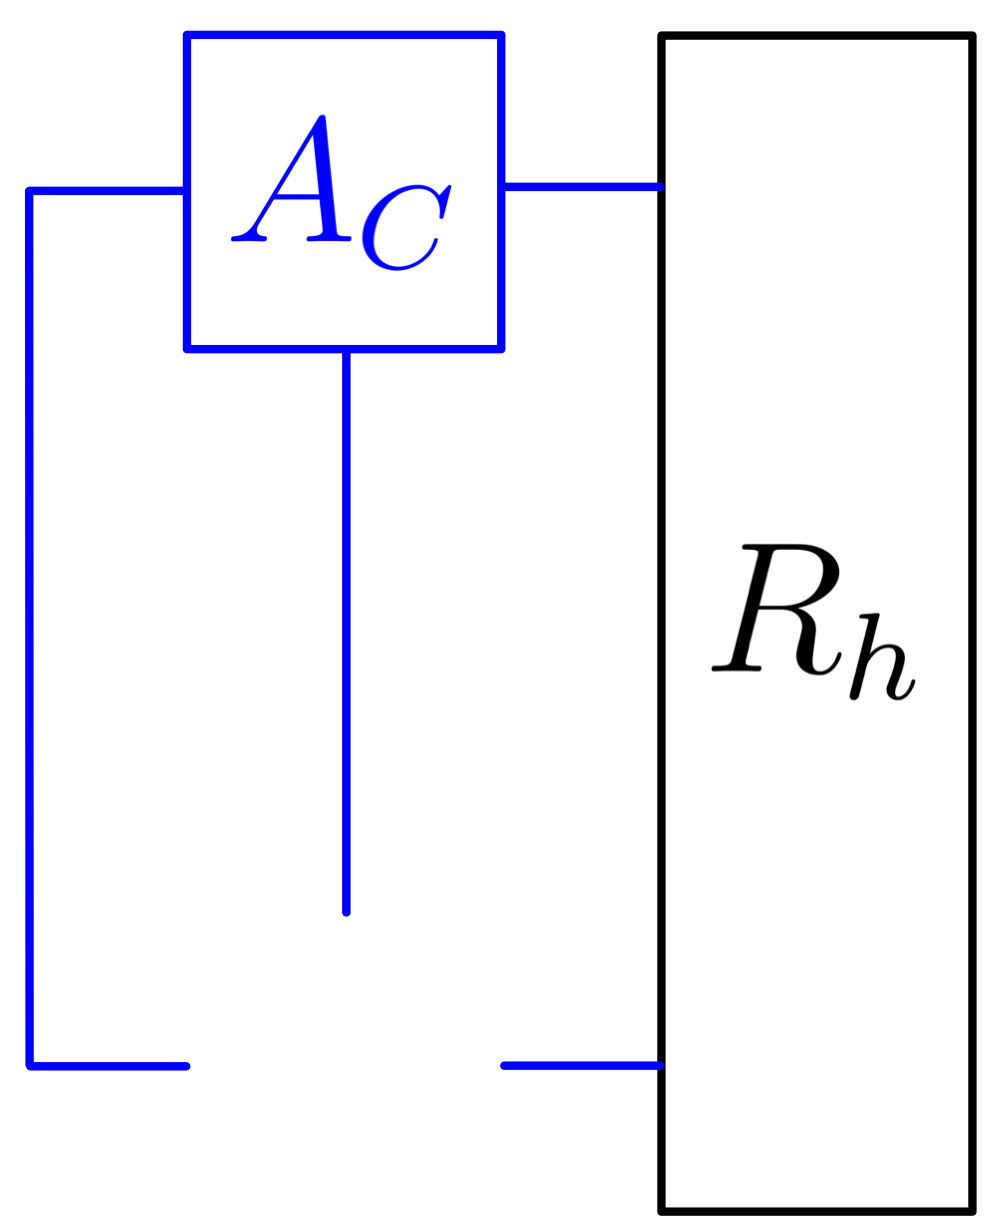
\includegraphics[height=3cm]{Heff1_4.png}} \hspace{0.2em},
\end{equation}
\begin{equation}
	\raisebox{-0.5\height}{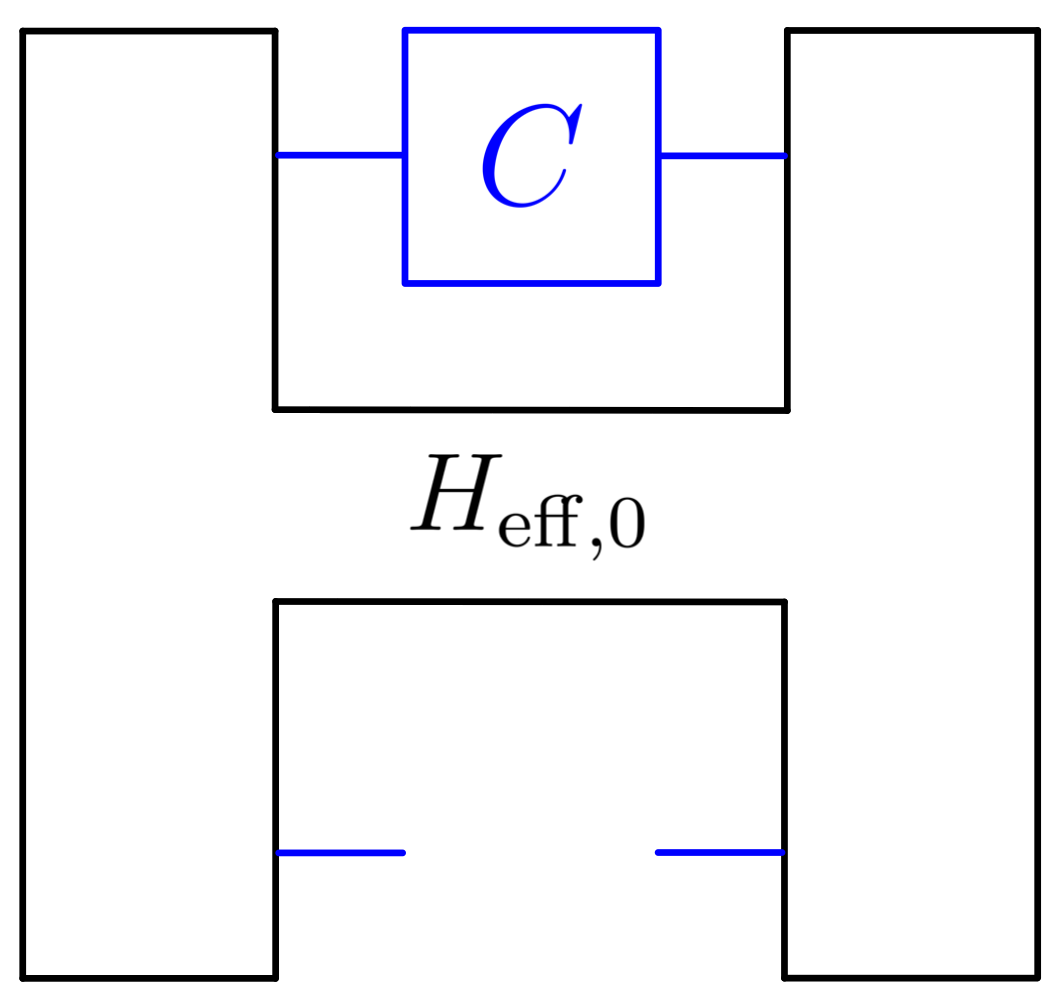
\includegraphics[height=3cm]{Heff0.png}} \: = \: \raisebox{-0.5\height}{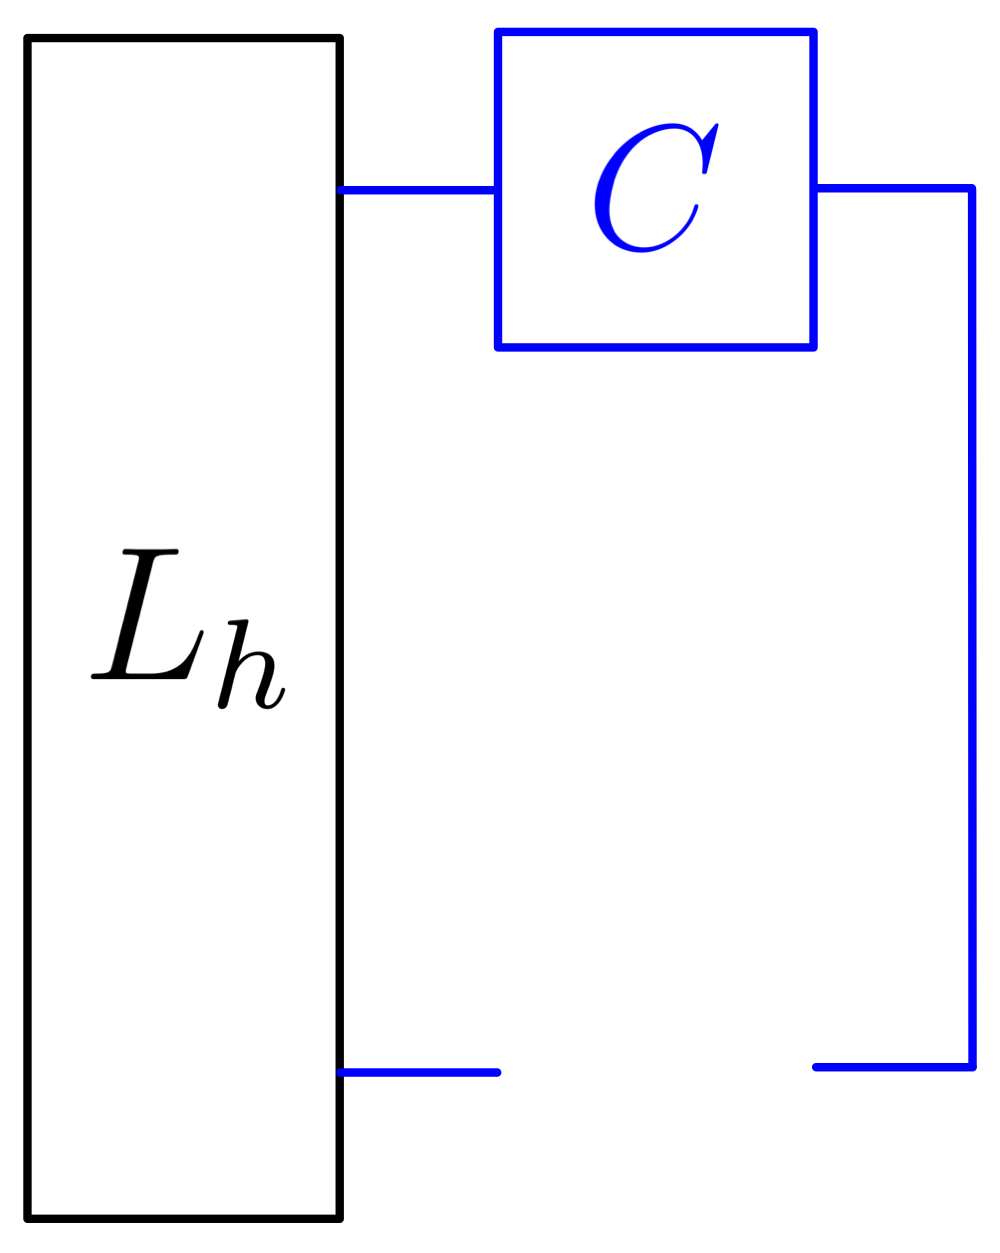
\includegraphics[height=3cm]{Heff0_1.png}} \: + \: \raisebox{-0.5\height}{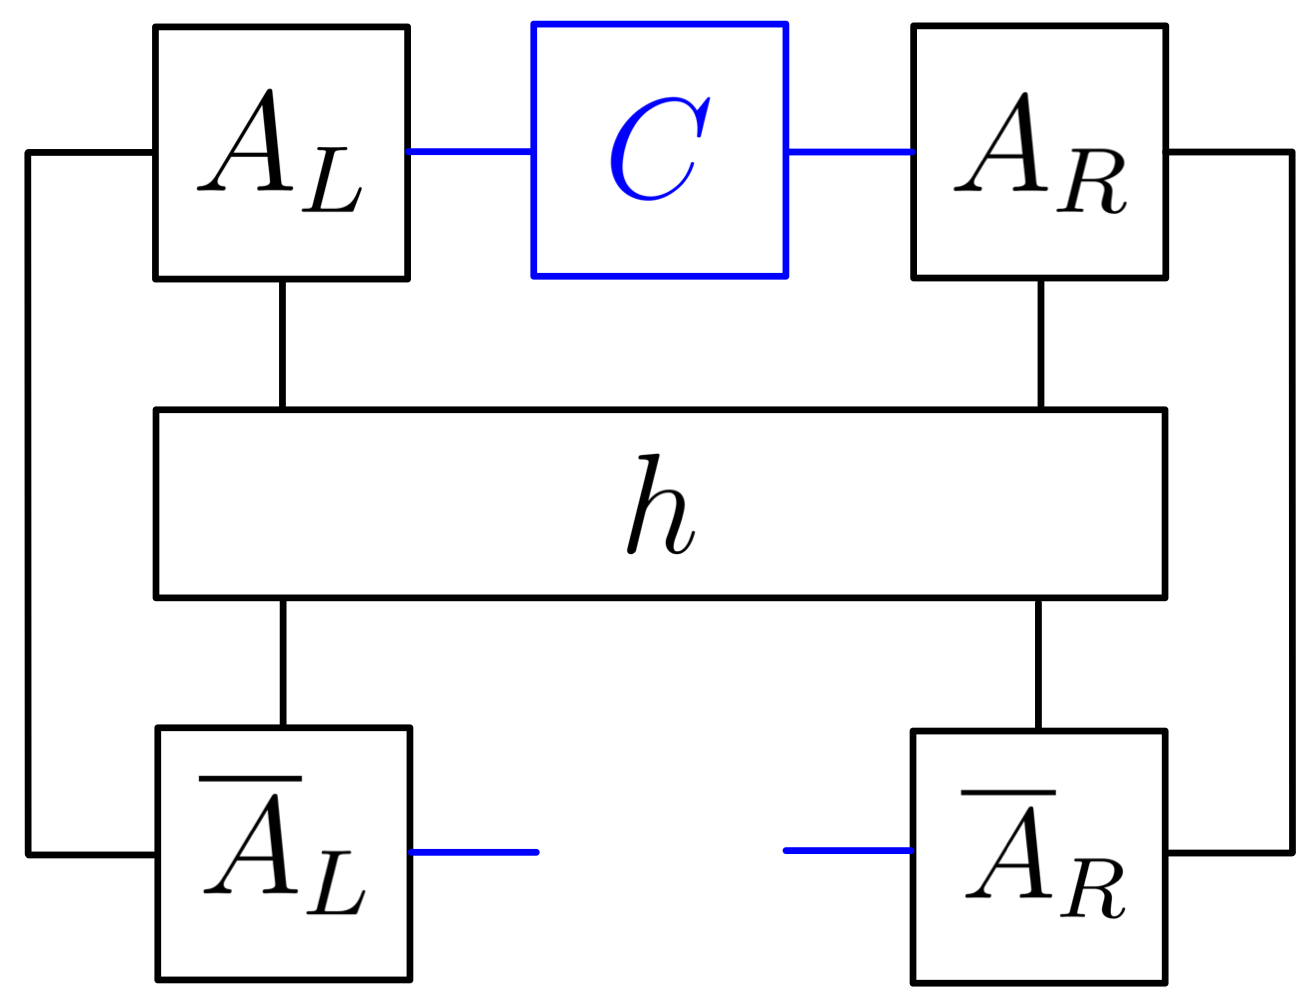
\includegraphics[height=3cm]{Heff0_2.png}} \: + \: \raisebox{-0.5\height}{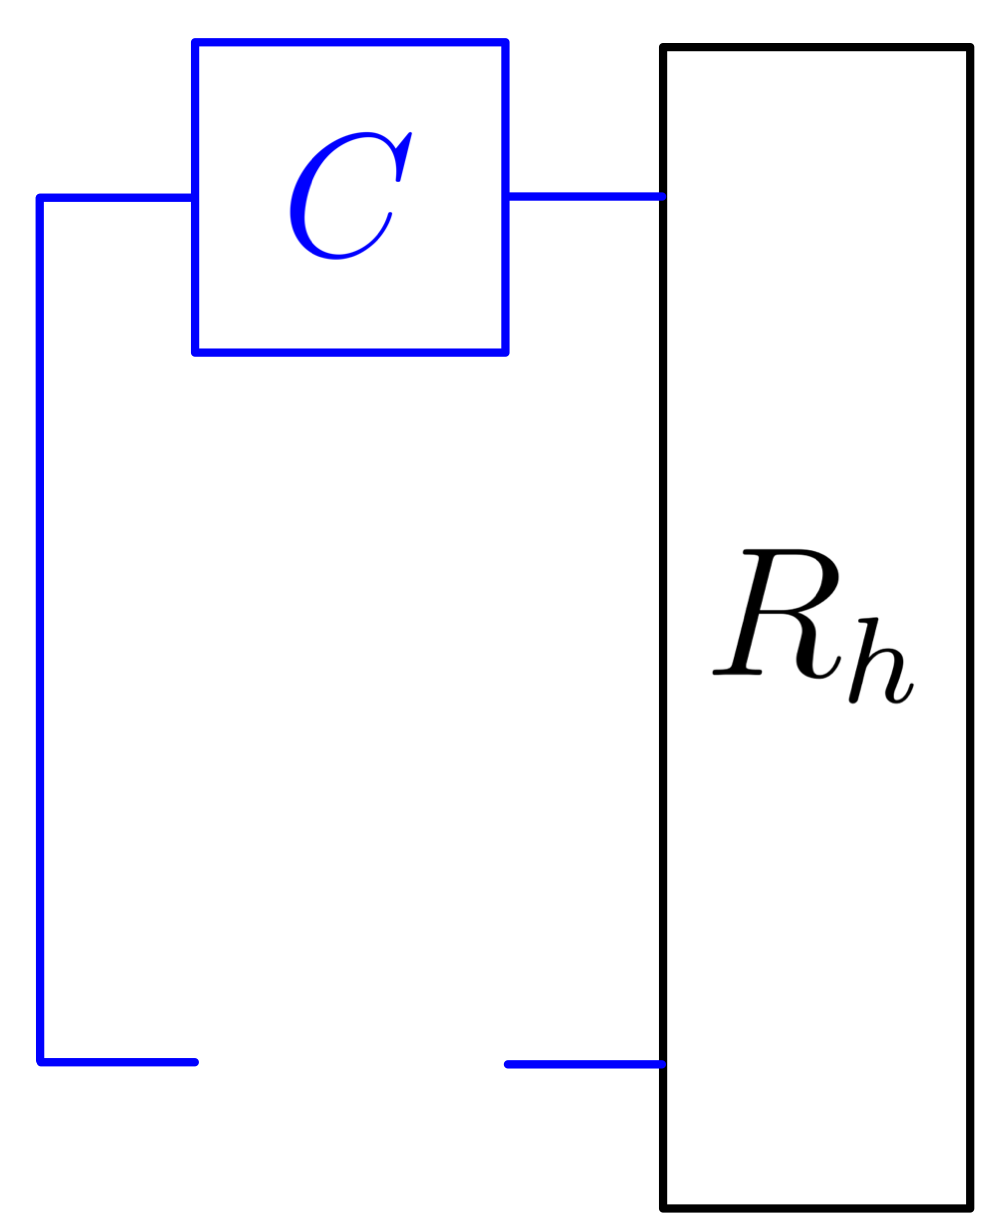
\includegraphics[height=3cm]{Heff0_3.png}} \hspace{0.2em}.
\end{equation}
All terms where $h$ acts only on sites left/right of $A_C$ or $C$, are additively summarized in the left/right boundary tensors
\begin{equation} \label{eq:Lh}
	\raisebox{-0.5\height}{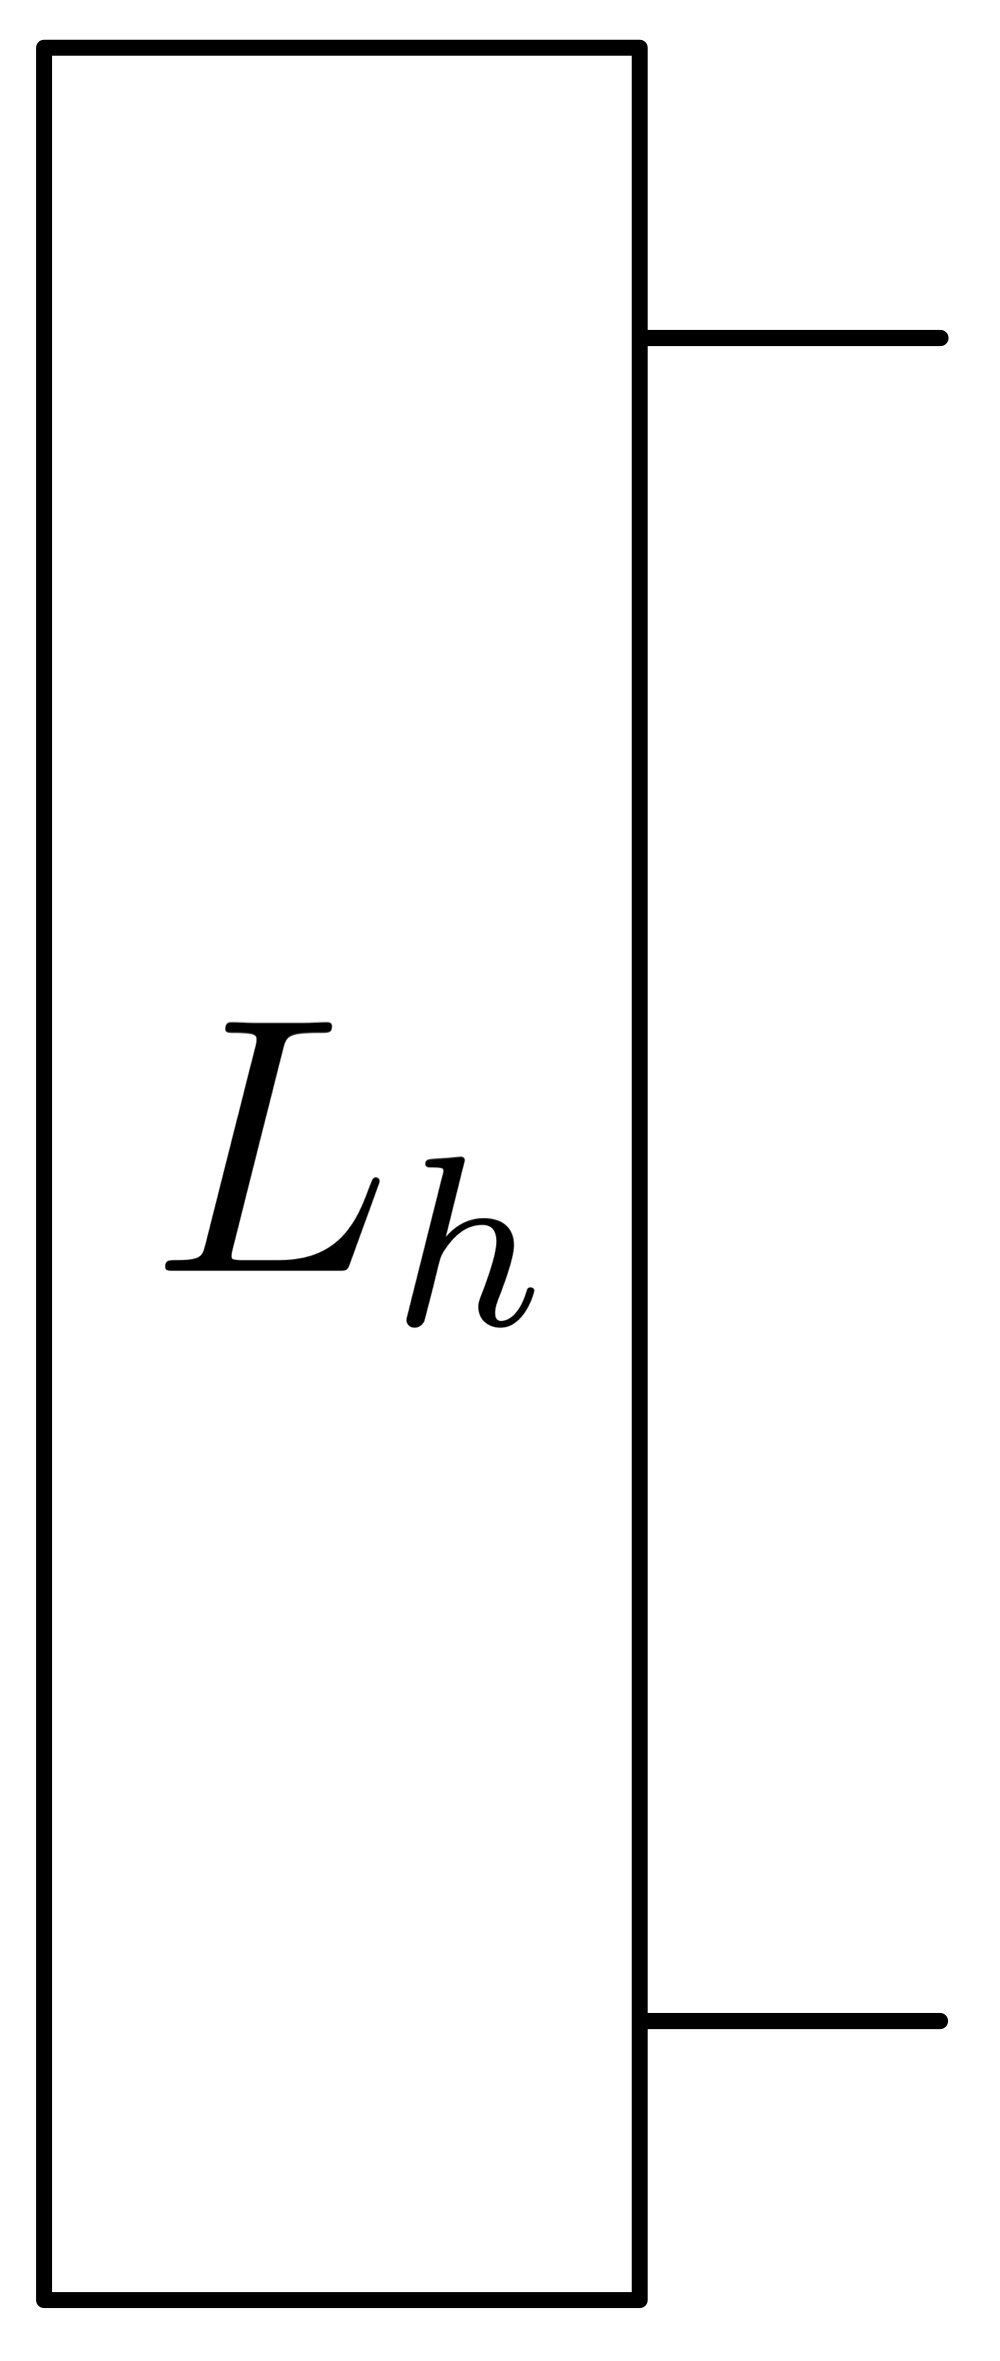
\includegraphics[height=3cm]{Lh.png}} 
	\: = \: 
	\raisebox{-0.5\height}{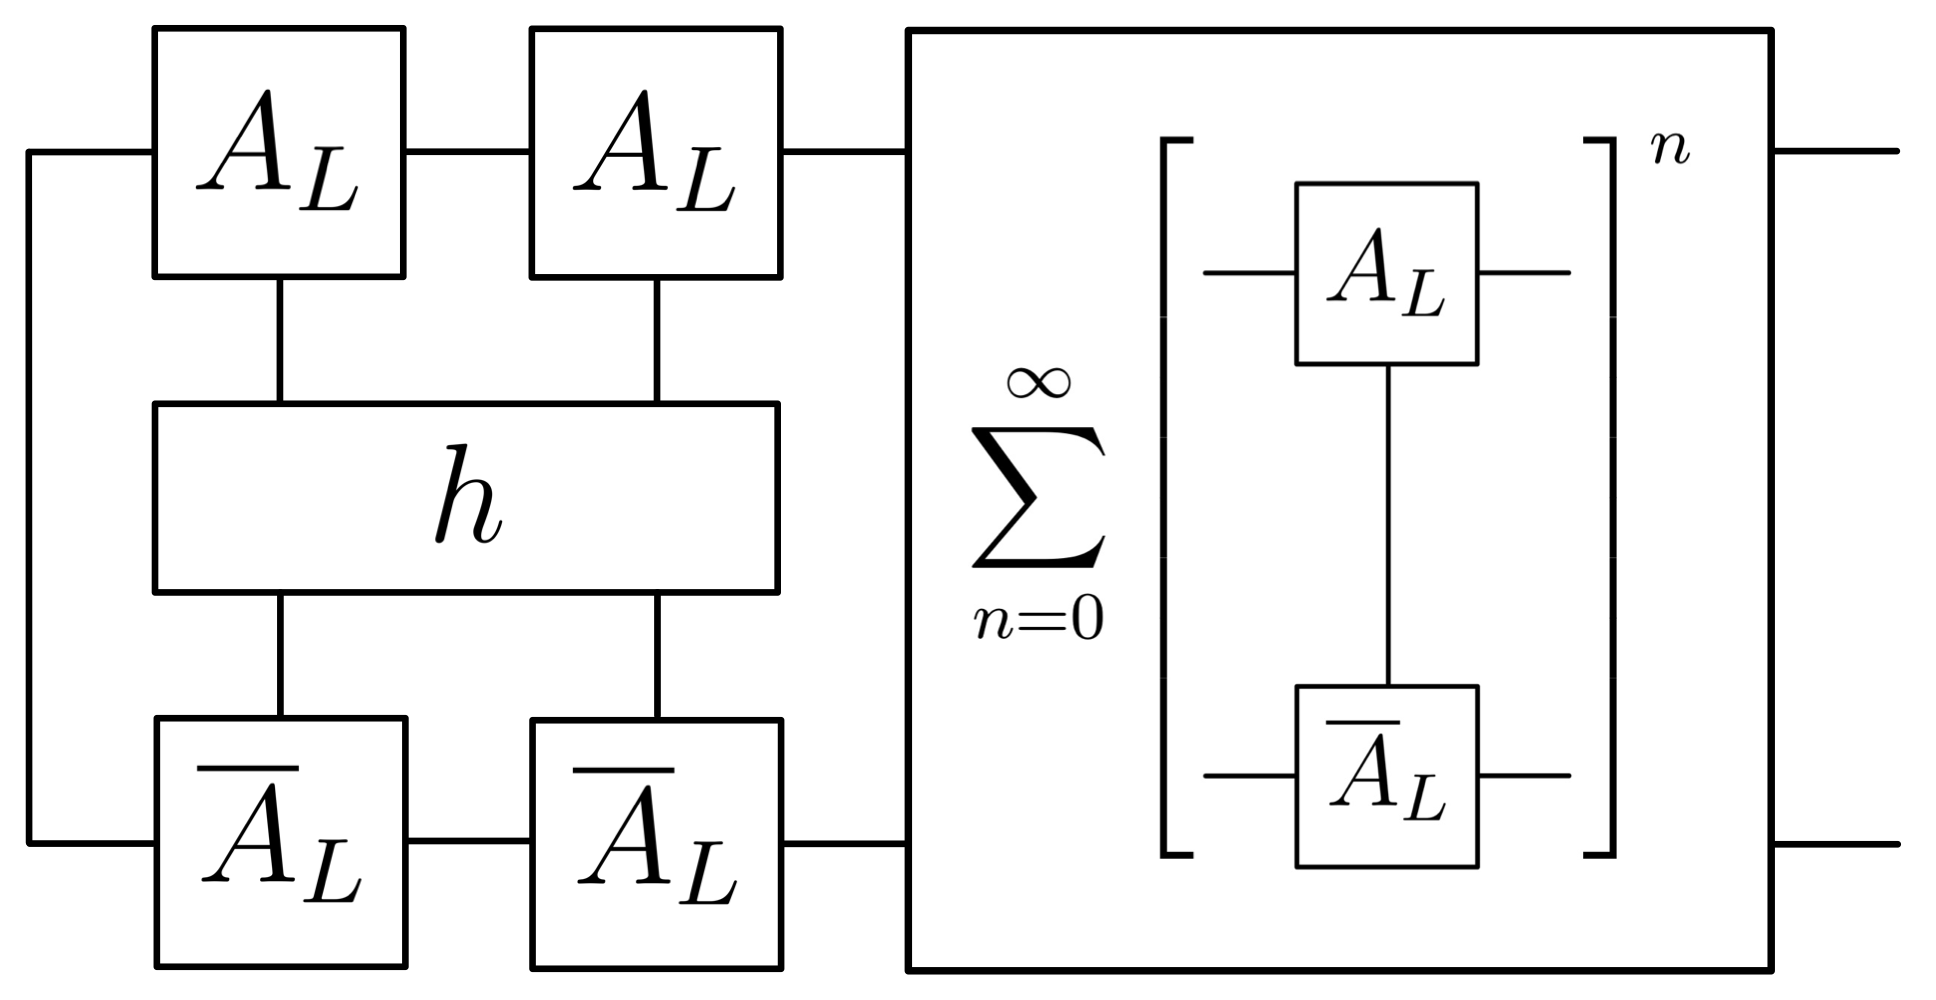
\includegraphics[height=3cm]{Lh_right.png}}
	\: = \: 
	\tbra{l_h} \sum_{n=0}^{\infty} [T_L]^n,
\end{equation}
\begin{equation} \label{eq:Rh}
	\raisebox{-0.5\height}{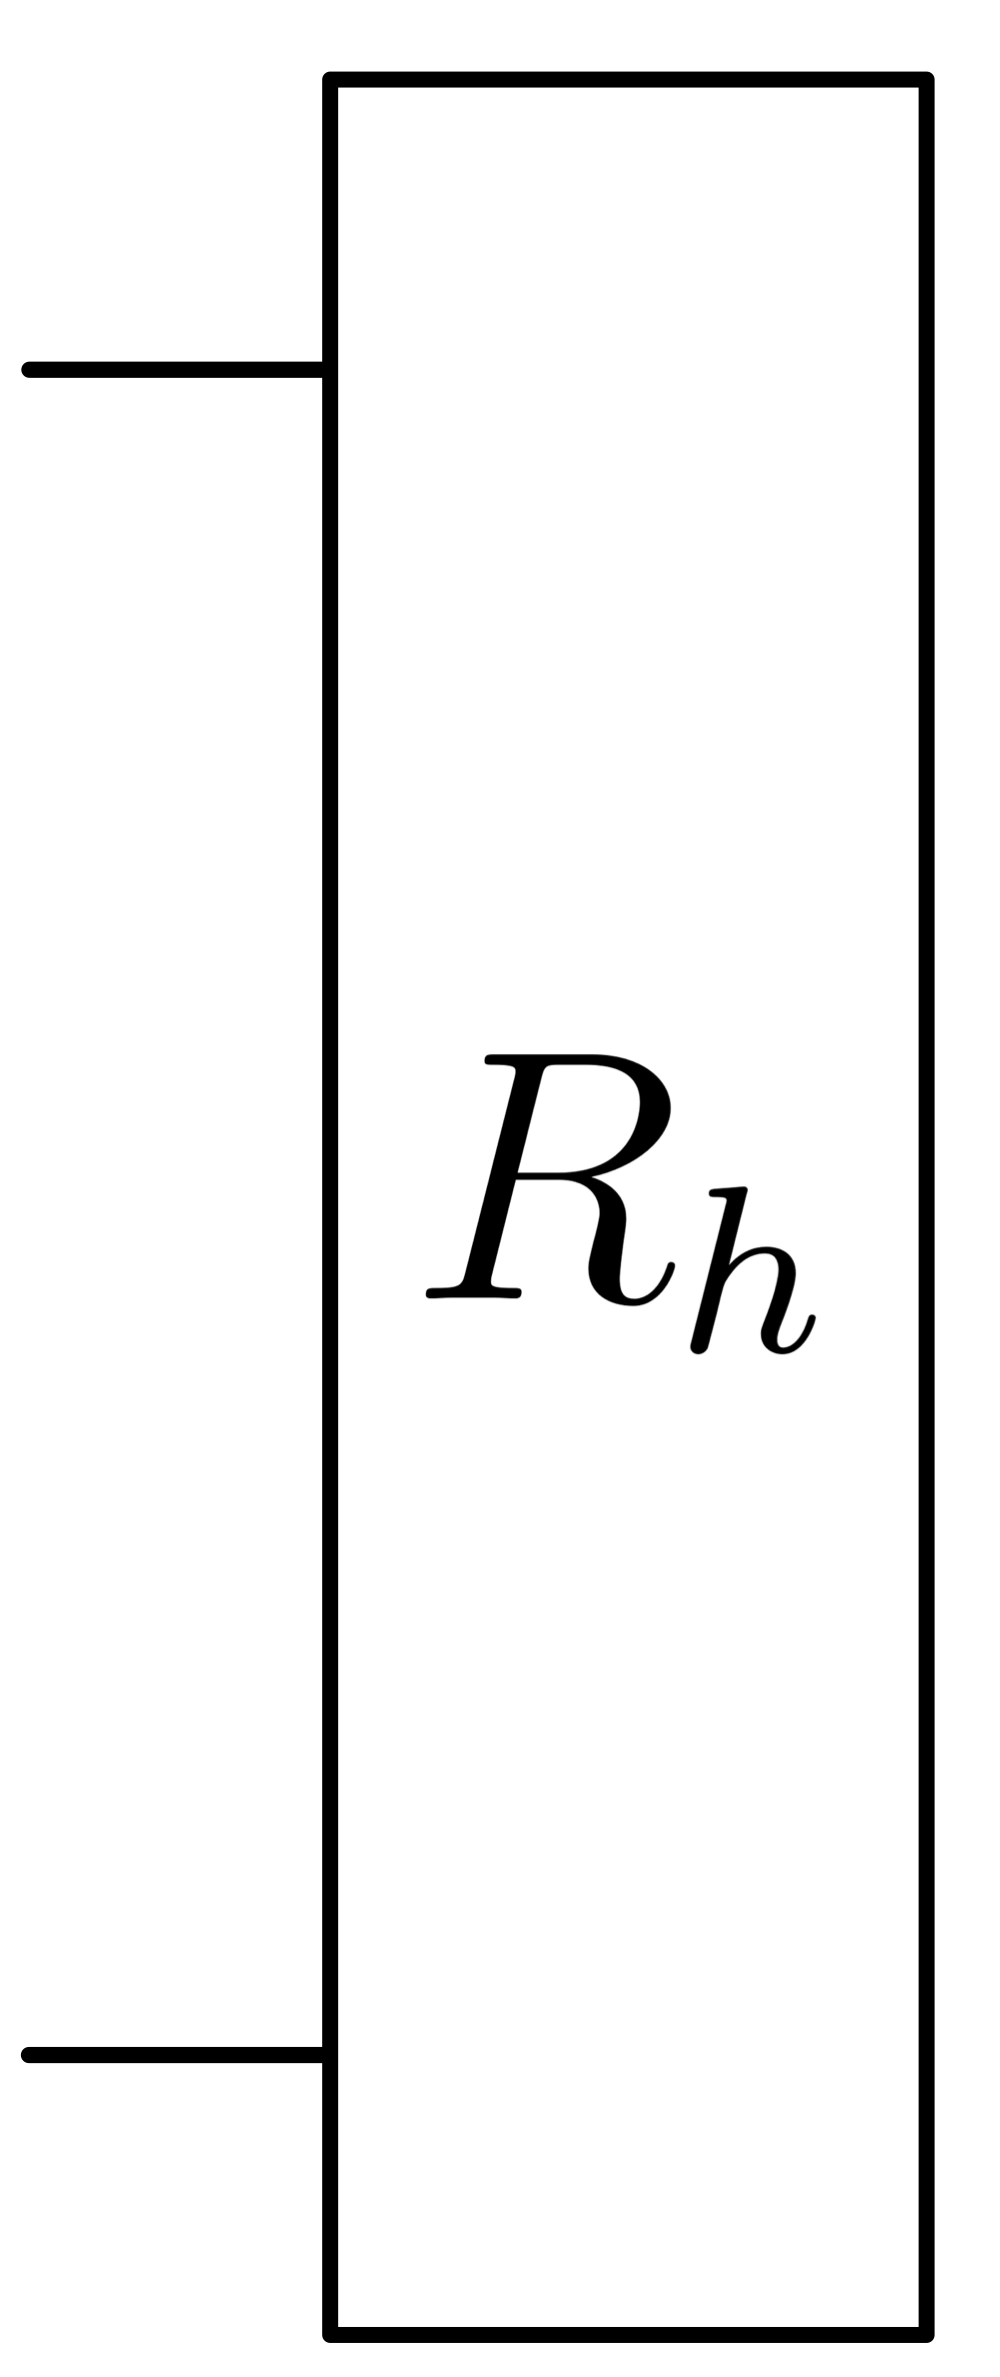
\includegraphics[height=3cm]{Rh.png}} 
	\: = \: 
 	\raisebox{-0.5\height}{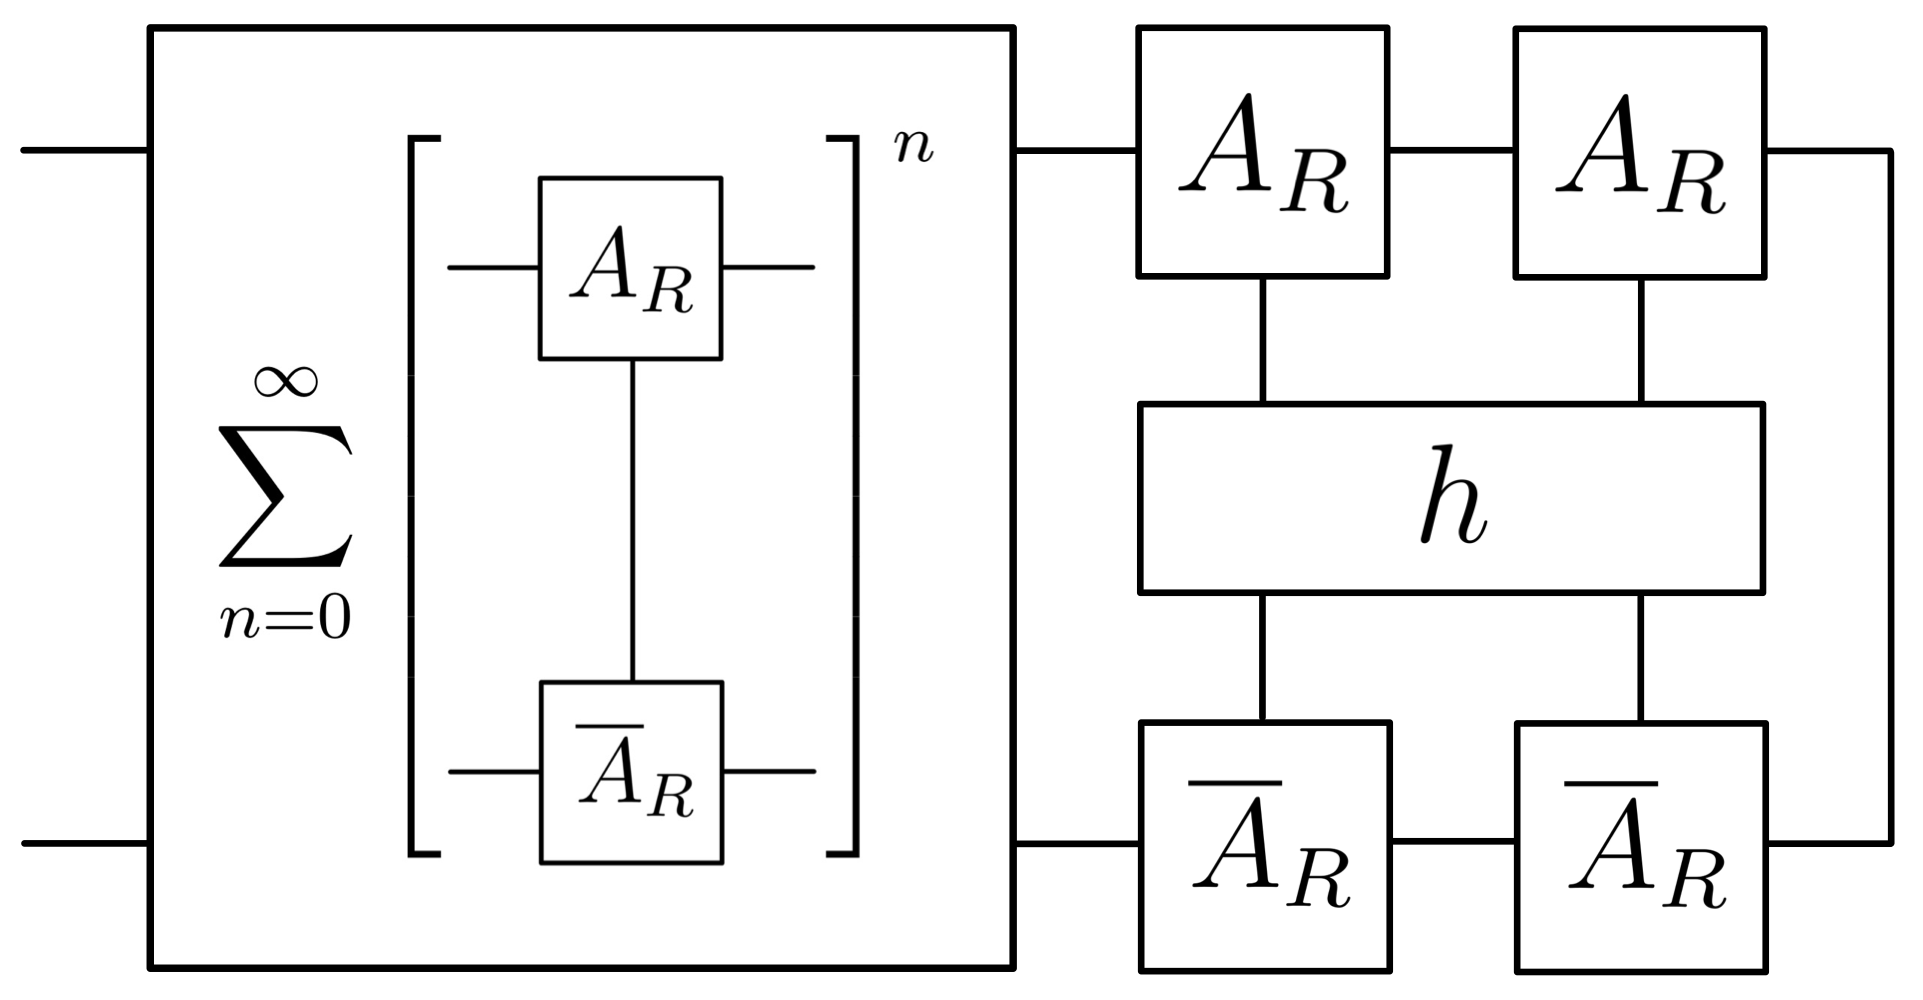
\includegraphics[height=3cm]{Rh_right.png}} 
	\: = \: 
	\sum_{n=0}^{\infty} [T_R]^n \tket{r_h}.
\end{equation}
\noindent To compute $L_h$ and $R_h$, we make explicit use of the primitivity property. For a general primitive transfer matrix $T = \tket{r} \tbra{l} + \mathcal{O}(\vert \lambda_2 \vert)$ with $\vert \lambda_2 \vert < 1$, we can compute the infinite geometric sum by separating the peripheral projector and using convergence for the residual operator:
\begin{align}
\begin{split}
	 \sum_{n=0}^{\infty} T^n &= \left[ \sum_{n=0}^{\infty} 1 \right] \tket{r} \tbra{l} + \sum_{n=0}^{\infty} \left[ T - \tket{r} \tbra{l} \right]^n \\
	 &= \vert \mathbb{N} \vert \tket{r} \tbra{l} + \left[ \mathbbm{1} - T + \tket{r} \tbra{l} \right]^{-1}.
\end{split}
\end{align}
For the left and right transfer matrices, $T_L = \tket{r} \tbra{\mathbbm{1}} + \mathcal{O}(\vert \lambda_2 \vert)$ and $T_R = \tket{\mathbbm{1}} \tbra{l} + \mathcal{O}(\vert \lambda_2 \vert)$, the formally diverging term $\propto \vert \mathbb{N} \vert$ corresponds to the total energy of the left and right half infinite chain, since 
\begin{equation}
	( l_h \vert r ) = ( l \vert r_h ) = e.
\end{equation}
By a constant energy shift $\Tilde{h} = h - e \mathbbm{1}$, we can ensure that the current state has energy density $\Tilde{e} = 0$ and avoid the extensive contribution. As a consequence, after having computed the nontrivial right and left eigenvectors $r$ and $l$, we can compute $L_h$ and $R_h$ as the solution of the following systems of linear equations:
\begin{equation} \label{eq:Lh_LE}
	\tbra{L_h} \left[ \mathbbm{1} - T_L + \tket{r} \tbra{\mathbbm{1}} \right] = \tbra{l_h},
\end{equation}
\begin{equation} \label{eq:Rh_LE}
	\left[ \mathbbm{1} - T_R + \tket{\mathbbm{1}} \tbra{l} \right] \tket{R_h} = \tket{r_h}.
\end{equation}
The variational ground state optimum, corresponding to $G = 0$ in \eqref{eq:projective_schrödinger_applied}, simultaneously satisfies the following conditions for the tensors $A_C$, $C$, $A_L$, $A_R$:
\begin{enumerate}[leftmargin=4em]
	\item[O1)] $\tket{A_C}$ ground state of $H_{\mathrm{eff}, 1}$,
	\item[O2)] $\tket{C}$ ground state of $H_{\mathrm{eff}, 0}$,
	\item[O3)] $A_C = A_L C = C A_R$.
\end{enumerate}
One update of the VUMPS (acronym for \textit{variational uniform matrix product states}) algorithm consists of
\begin{enumerate}[label=A\arabic*), ref=A\arabic*, leftmargin=4em]
	\item $\tket{A_C}$ $\rightarrow$ ground state of $H_{\mathrm{eff}, 1}$ \label{item:vumps_1},
	\item $\tket{C}$ $\rightarrow$ ground state of $H_{\mathrm{eff}, 0}$ \label{item:vumps_2}, 
	\item $A_L$/$A_R$ from right/left polar decompositions of $A_C$ and $C$ \label{item:vumps_3}. 
\end{enumerate}
For a fixed bond dimension $D$, we bring a random, primitive tensor (with spectral radius one) into canonical form and repeat the steps \ref{item:vumps_1})--\ref{item:vumps_3}) until convergence in gradient norm up to tolerance tol:
\begin{equation} \label{eq:gradient_norm}
	\mathcal{E}_{\mathrm{VUMPS}} = \Vert G \Vert_2 = \Vert H_{\mathrm{eff},1}(A_C) - A_L H_{\mathrm{eff},0}(C) \Vert_2 < \mathrm{tol}.
\end{equation}
A few comments about the VUMPS algorithm: 
\begin{itemize}
	\item To make the implementation efficient, we solve the effective eigenvalue problems \ref{item:vumps_1}) and \ref{item:vumps_2}) with an iterative Lanczos method, which only needs to know the effect of $H_{\mathrm{eff}, 1}$ and $H_{\mathrm{eff}, 0}$ on $\tket{A_C}$ and $\tket{C}$, respectively. Previous tensors are used as initial guesses. In the same way, we use iterative Arnoldi methods to compute the eigenvectors $r$, $l$ of the (non-Hermitian) transfer matrices $T_L$, $T_R$ and to solve the linear equations \eqref{eq:Lh_LE}, \eqref{eq:Rh_LE}. As a consequence, the computational time complexity of  the VUMPS algorithm scales as $\mathcal{O}(D^3)$.
	\item Before convergence, the canonical form $A_C = A_L C = C A_R$ is not exactly fulfilled. If it was, $r = C C^{\dagger}$ and $l = C^T \overline{C}$ would be the nontrivial right and left eigenvectors of $T_L$ and $T_R$, needed for \eqref{eq:Lh_LE} and \eqref{eq:Rh_LE}. Nevertheless, we can use them as initial guesses for the Arnoldi iterations.
	\item We still have to specify \ref{item:vumps_3}). In exact arithmetic, the solution of the minimization problems 
\begin{equation}
	\min_{A_L^{\dagger} A_L = \mathbbm{1}} \Vert A_C - A_L C\Vert_2, \:\: \min_{A_R A_R^{\dagger} = \mathbbm{1}} \Vert A_C - C A_R \Vert_2
\end{equation}
is known: $A_L$ is equal to the isometry in the right polar decomposition of $A_C C^{\dagger}$, $A_R$ is equal to the isometry in the left polar decomposition of $C^{\dagger} A_C$. But this involves the square of the singular values of $C$, which might fall below machine precision. An alternative that is robust in finite precision arithmetic (and still close to optimal) is given by the following computation from separate polar decompositions of $A_C$ and $C$:
\begin{align}
	& \mathbb{C}^{Dd \times D} \owns A_C \overset{\mathrm{rP}}{=} U_{L, 1} P_{L, 1} \text{ and } C \overset{\mathrm{rP}}{=} U_{L, 0} P_{L, 0} \: \Rightarrow \: A_L = U_{L, 1} U_{L, 0}^{\dagger}, \\
	& \mathbb{C}^{D \times dD} \owns A_C \overset{\mathrm{lP}}{=} P_{R, 1} U_{R, 1} \text{ and } C \overset{\mathrm{lP}}{=} P_{R, 0} U_{R, 0} \: \Rightarrow \: A_R = U_{R, 0}^{\dagger} U_{R, 1}.
\end{align}
	\item In contrast to iDMRG, which successively grows the lattice by updated unit cells, VUMPS truly solves the variational problem in the sense of completely updating the state with each iteration and consequently keeping the translation invariance at any time.
\end{itemize}

% benchmark
\begin{figure}[t]
  \centering
  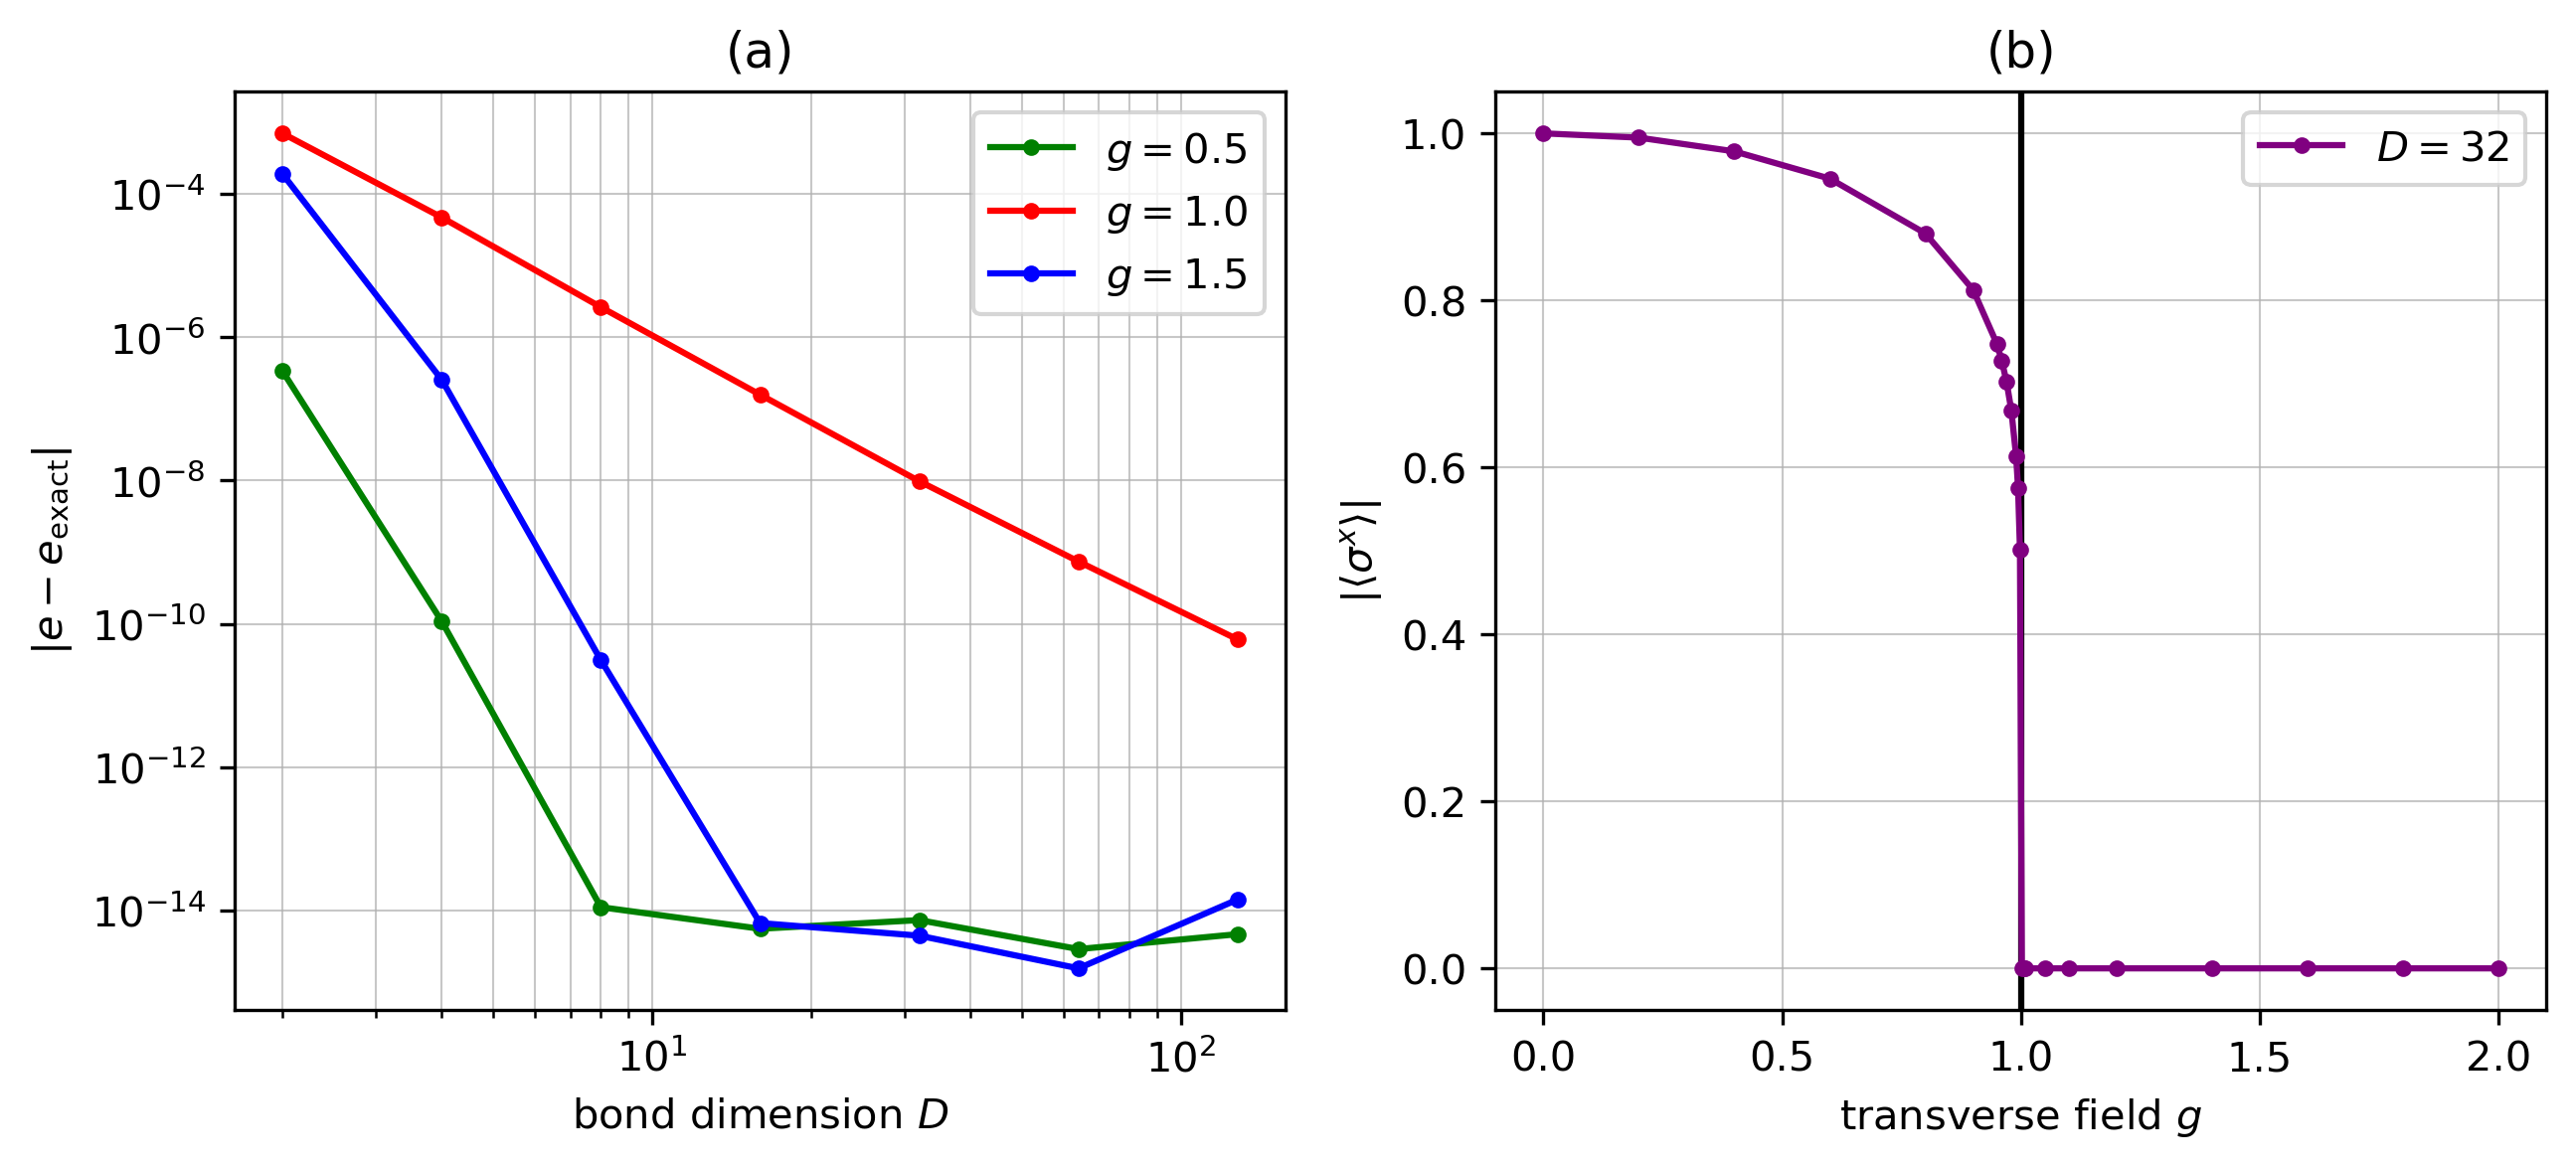
\includegraphics[width=1.0\linewidth]{vumps.png}
  \caption{TFI benchmark for the VUMPS algorithm with tolerance $10^{-12}$ in gradient norm. In the left panel (a), we plot the energy density error $\Delta e = \vert e - e_{\mathrm{exact}} \vert$ against increasing bond dimension on a log-log scale. In the gapped phases with representative transverse field values $g = 0.5$ and $g = 1.5$, the error falls below machine precision quickly. At the critical point $g = 1$, the error exhibits a power law scaling with $D$. In the right panel (b), we show the sharp transition to zero magnetization density at $g= 1$, obtained for $D = 32$.}
 \label{fig:vumps}
\end{figure}
\noindent \underline{Benchmark} \\[0.5em]
\noindent We now benchmark the VUMPS algorithm with the TFl model, for which the ground state energy density can be exactly computed with Jordan-Wigner and Bogoliubov transformations (as summarized in section \ref{sec:tfi_exact_solution}):
\begin{equation}
	e_{\mathrm{exact}} = - \frac{1}{2 \pi} \int_{-\pi}^{\pi} dp \: \frac{\epsilon_p}{2} 
	\:\overset{J=1}{=}\:
	 - \frac{1}{2 \pi} \int_{-\pi}^{\pi} dp \sqrt{g^2 - 2g \cos (p) + 1}.
\end{equation}
For a tolerance of $10^{-12}$ in gradient norm \eqref{eq:gradient_norm}, and different bond dimensions $D$, we run VUMPS to get an approximate ground state with energy density $e$. We plot the convergence of the energy error $\Delta e = \vert e - e_{\mathrm{exact}} \vert$ against $D$ on a log-log scale, for the three representative transverse field values $g = 0.5$ (ferromagnetic phase), $g = 1.0$ (critical point) and $g = 1.5$ (paramagnetic phase). The results are shown in the left part (a) of figure \ref{fig:vumps}. In the gapped phases $g \neq 1$, the error falls below machine precision already at modest bond dimensions ($D \approx 16$). At the critical point $g = 1$, the error exhibits a power law scaling with $D$, in agreement with the theory of finite entanglement scaling at one-dimensional quantum critical points \cite{pollmann2009theory}. \\[0.5em]
\noindent For our purposes, an energy accuracy of $10^{-8}$ and therefore a bond dimension of $D = 32$ is sufficient for all values of $g$. In the right panel (b) of figure \ref{fig:vumps}, the magnetization density $m = \vert \langle \sigma^x \rangle \vert$ of the VUMPS ground state serves as an order parameter for the TFI quantum phase diagram. As expected from section \ref{sec:tfi_phase_diagram}, starting from $m = 1$ at $g = 0$, quantum fluctuations reduce $m$ as $g$ is increased and lead to a sharp drop to $m = 0$ at the critical point $g=1$.


% VARIATIONAL PLANE WAVE EXCITATIONS
\section{Variational plane wave excitations (VPWE)} \label{sec:uexcitations}
Seeing the uMPS ground state $\ket{\psi (A)}$ as correlated background, we create a single quasiparticle excitation on top by inserting local tensor perturbations in a momentum plane wave superposition \cite{haegeman2012variational, vanderstraeten2019tangent}:
\begin{equation} \label{eq:uexcitation_ansatz}
	\ket{\psi_p(B; A)} = \sum_{n \in \mathbb{Z}} \textcolor{blue}{e^{ipn}} \raisebox{-0.5\height}{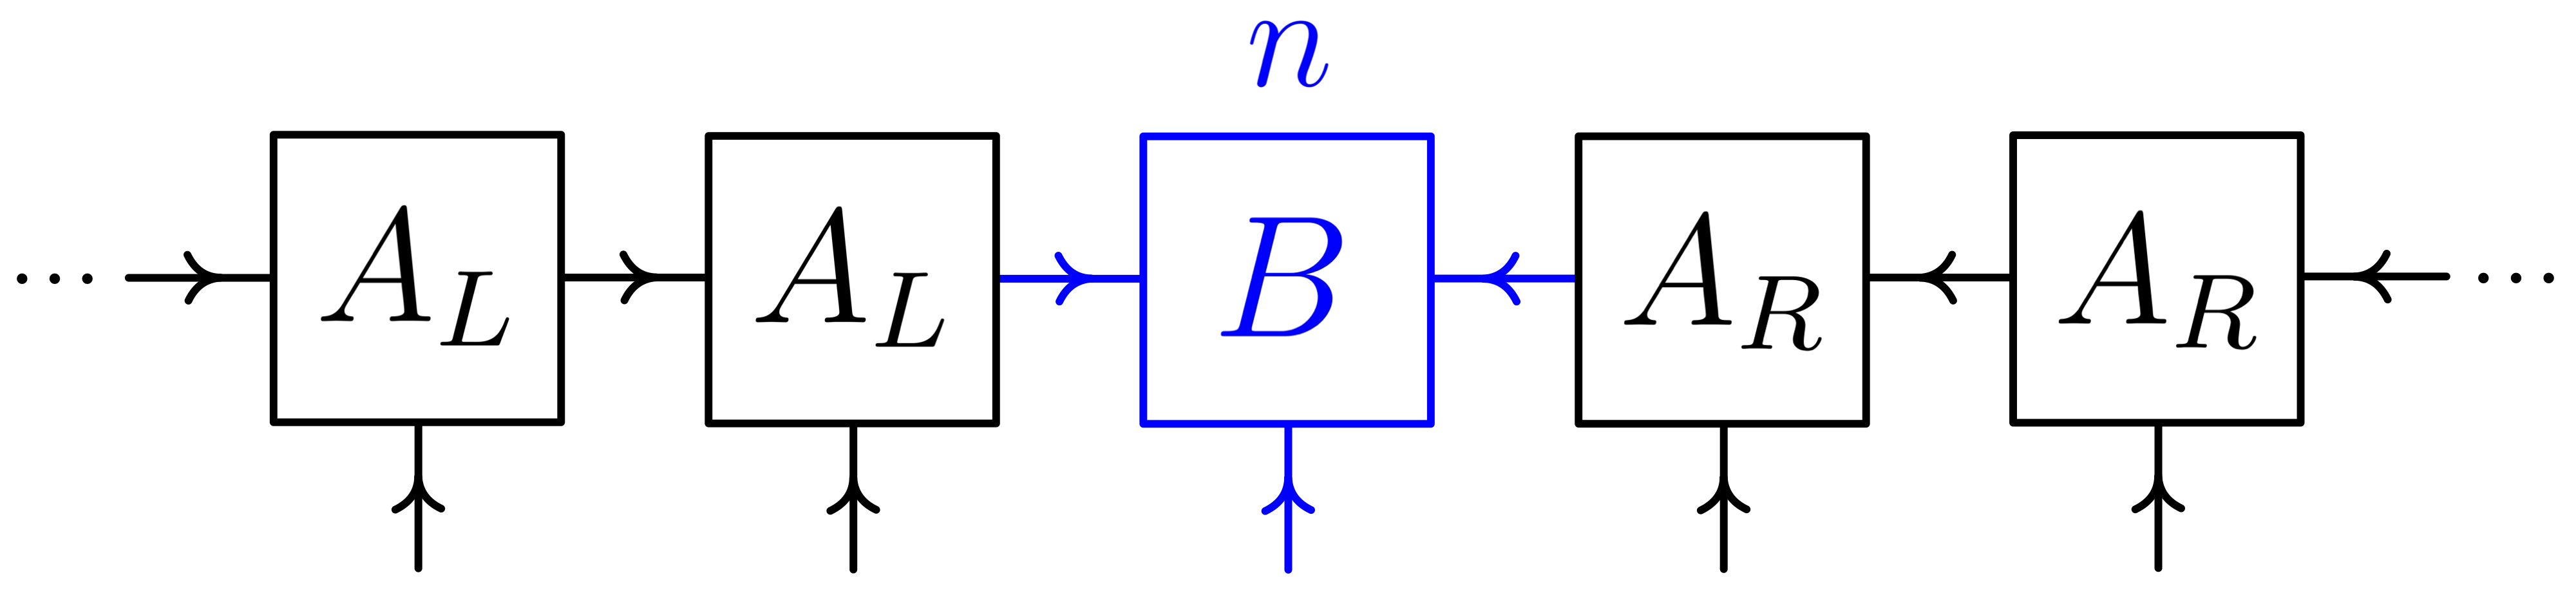
\includegraphics[height=1.4cm]{tangent_vector_canonical_normalized.png}} \hspace{0.2em} .
\end{equation}

% gauge fixing
\noindent \underline{Gauge fixing} \\[0.5em]
Our ansatz \eqref{eq:uexcitation_ansatz} is a boosted version of the tangent space vector \eqref{eq:tangent_space_vector_canonical}, with slightly modified gauge freedom:
\begin{equation}
	B \rightarrow B + A_L Y - e^{-ip} Y A_R
\end{equation}
leaves the state invariant for any $Y \in \mathbb{C}^{D \times D}$. Again, we fix the $D^2$ gauge parameters by the effective parametrization
\begin{equation} \label{eq:uexcitation_gauge}
	\raisebox{-0.55\height}{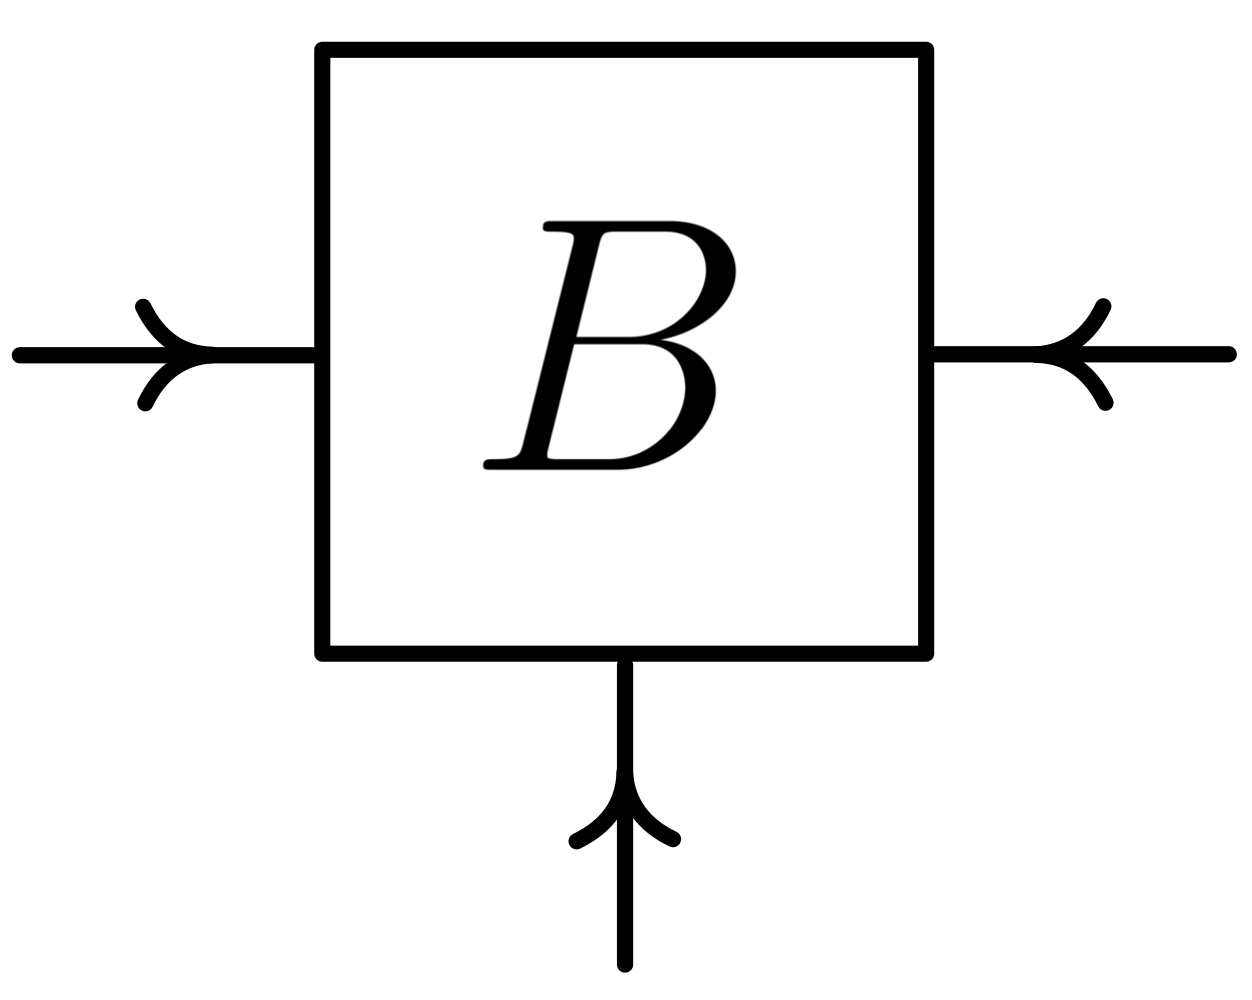
\includegraphics[height=1.2cm]{B_normalized.png}} \: = \: \raisebox{-0.55\height}{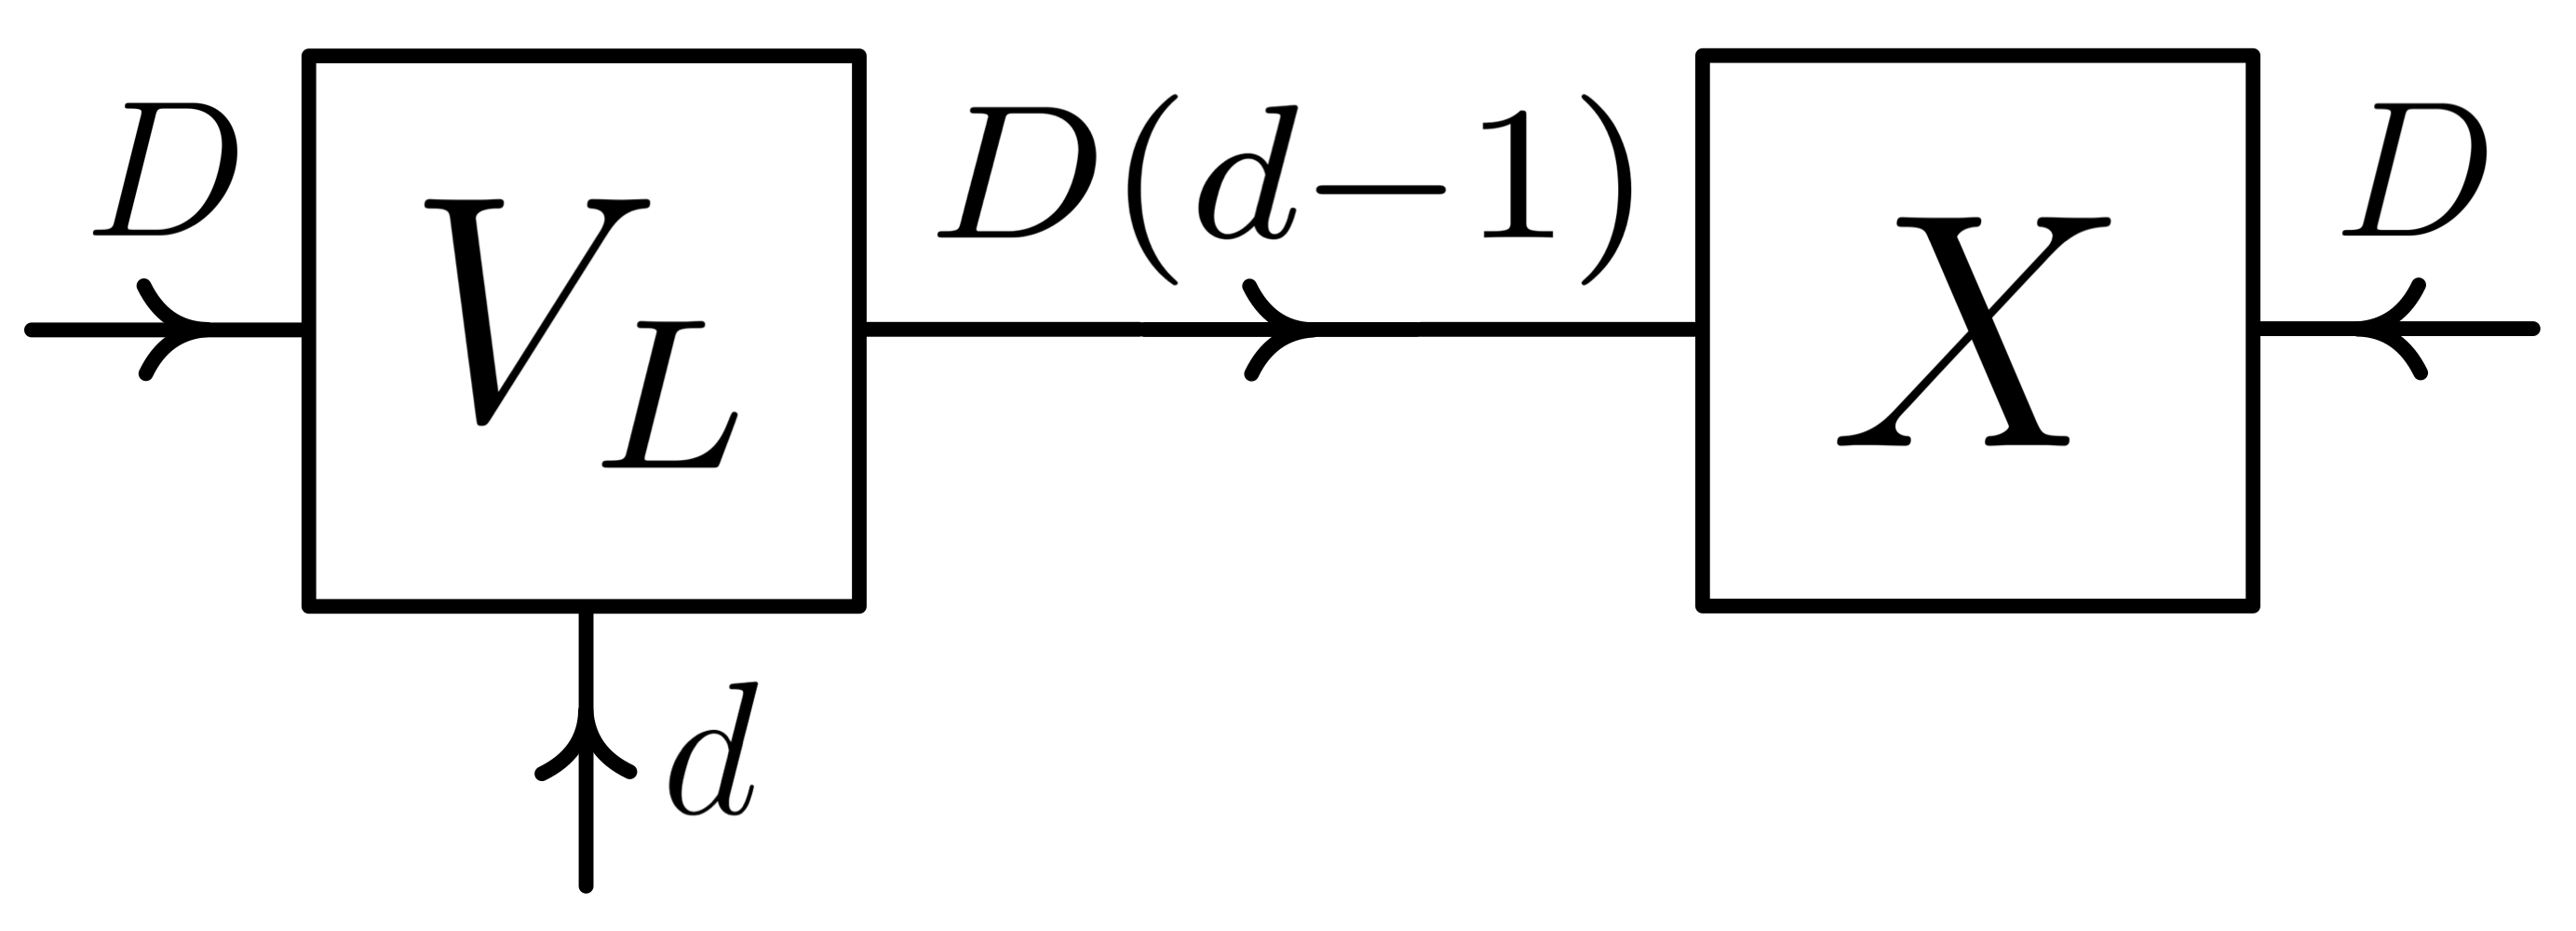
\includegraphics[height=1.2cm]{VL_X_normalized.png}} \:\: \text{ with } \:\: \raisebox{-0.45\height}{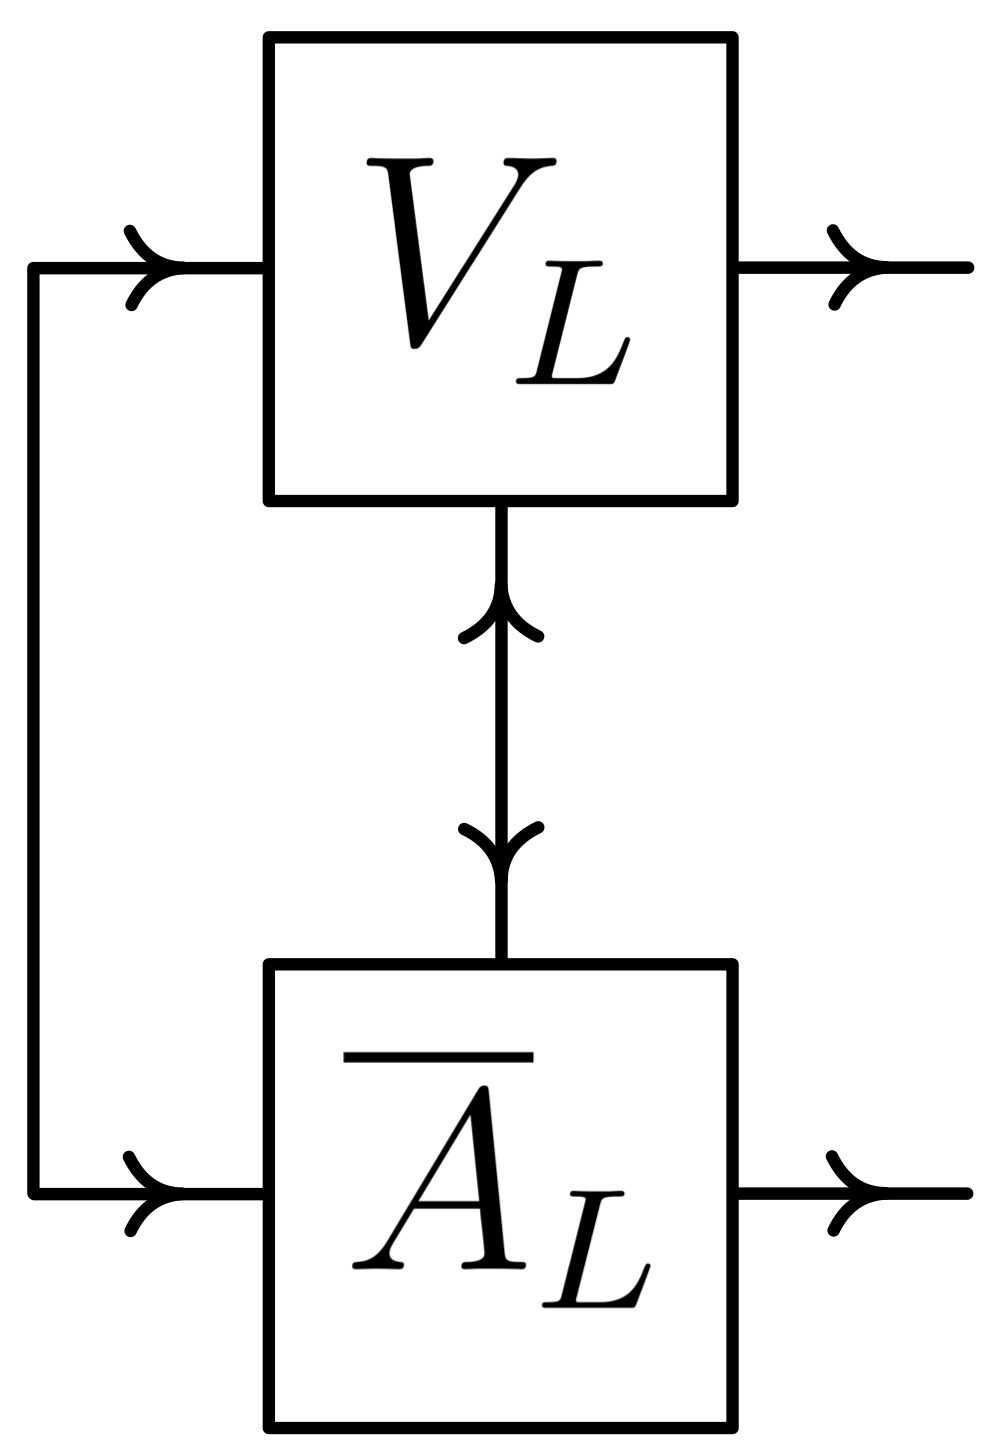
\includegraphics[height=2.2cm]{VL_AL.png}} = 0.
\end{equation}
This has two crucial implications. First, it ensures that the excitations 
\begin{equation} \label{eq:plane_wave_excitations}
	\ket{\psi_p(X; A)} = \sum_{n \in \mathbb{Z}} \textcolor{blue}{e^{ipn}} \raisebox{-0.5\height}{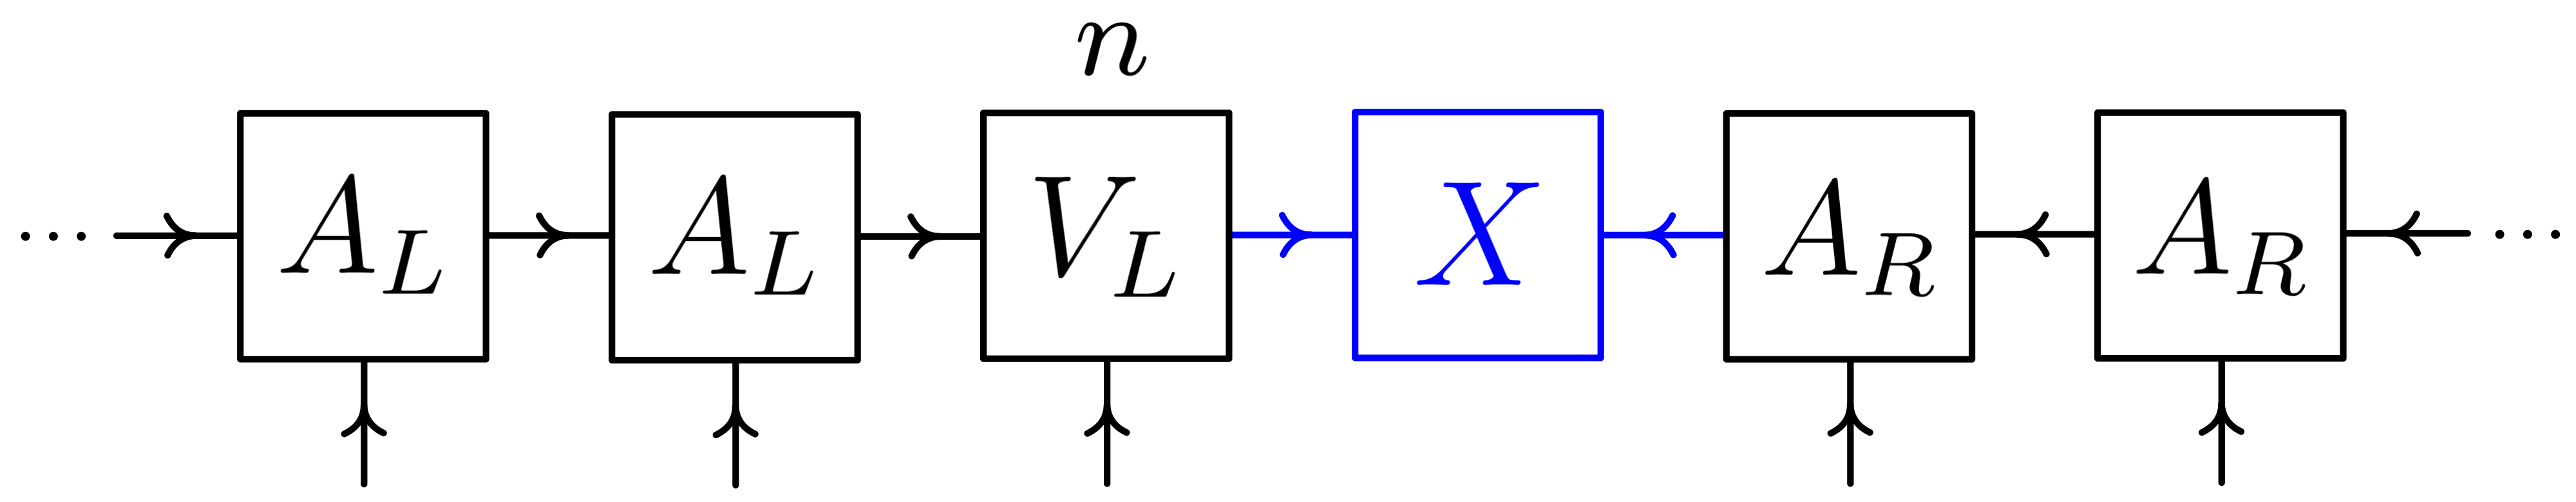
\includegraphics[height=1.4cm]{tangent_vector_X_normalized.png}} \hspace{0.2em} 
\end{equation}
are orthogonal to the ground state by construction:
\begin{equation} \label{eq:excitation_gs_overlap}
	\langle \psi (\overline{A}) \vert \psi_p (X; A) \rangle = 0 \text{ for all } p, X.
\end{equation}
Second, it implies that the overlap between two excitations is given by
\begin{equation} \label{eq:excitation_overlap}
	\langle \psi_k (\overline{Y}; A) \vert \psi_p (X; A) \rangle = 2 \pi \delta (p-k) (\overline{Y} \vert X ).
\end{equation}
For this we used the following relation, which reduces a double sum over $n, l \in \mathbb{Z}$ to a single one, for any quantity $f$ that only depends on the distance $n - l$:
\begin{equation} \label{eq:double_sum}
	\sum_{n, l \in \mathbb{Z}} e^{ipn} e^{-ikl} f(n-l) \overset{m=n-l}{=} \sum_{l\in \mathbb{Z}} e^{i(p-k)l} \sum_{m \in \mathbb{Z}}e^{ipm} f(m) = 2 \pi \delta (p-k) \sum_{m \in \mathbb{Z}} e^{ipm} f(m).
\end{equation}
From \eqref{eq:excitation_overlap} we can conclude that the gauge \eqref{eq:uexcitation_gauge} orthogonalizes excitations with different momenta and removes \textit{zero modes}, i.e. nonzero tensors $B_0 = A_L Y - e^{-ip} Y A_R \neq 0$ that correspond to zero states $\ket{\psi_p (B_0; A)} = 0$. As a consequence, for a fixed momentum $p$, the plane wave excitations \eqref{eq:plane_wave_excitations} are well-defined for a variational minimization of the energy with respect to $X$:
\begin{equation}
	\argmin_{X \in \mathbb{C}^{D(d-1) \times D}} \frac{\bra{\psi_p(\overline{X}; \overline{A})} H \ket{\psi_p(X; A)}}{\langle \psi_p(\overline{X}; \overline{A}) \vert \psi_p(X; A) \rangle}.
\end{equation}

% effective hamiltonian
\noindent \underline{Effective Hamiltonian} \\[0.5em]
\noindent Again making use of \eqref{eq:double_sum}, the stationary condition \eqref{eq:stationary_condition} becomes 
\begin{equation} \label{eq:excitation_minimization}
	2 \pi \delta (0) \: \partial_{\overline{X}} \left[( \overline{X} \vert H_{\mathrm{eff}}(p) \vert X ) - \lambda ( \overline{X} \vert X ) \right] = 0.
\end{equation}
The effective Hamiltonian $H_{\mathrm{eff}}(p)$ acts on $X$ as follows:
\begin{equation} \label{eq:Heff_p}
	\raisebox{-0.5\height}{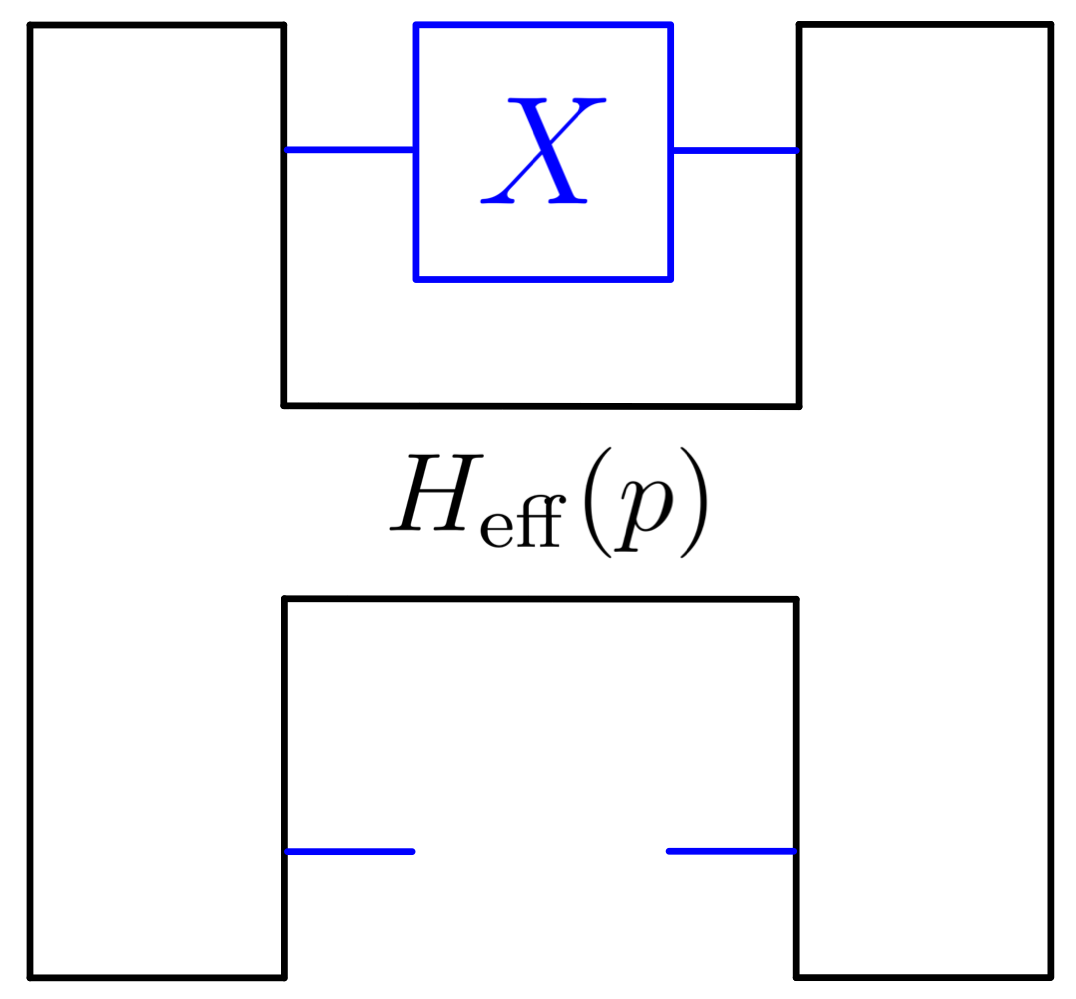
\includegraphics[height=3cm]{Heff_p.png}} 
	= \sum_{n, m \in \mathbb{Z}} \textcolor{blue}{e^{ipm}} 
	\raisebox{-0.5\height}{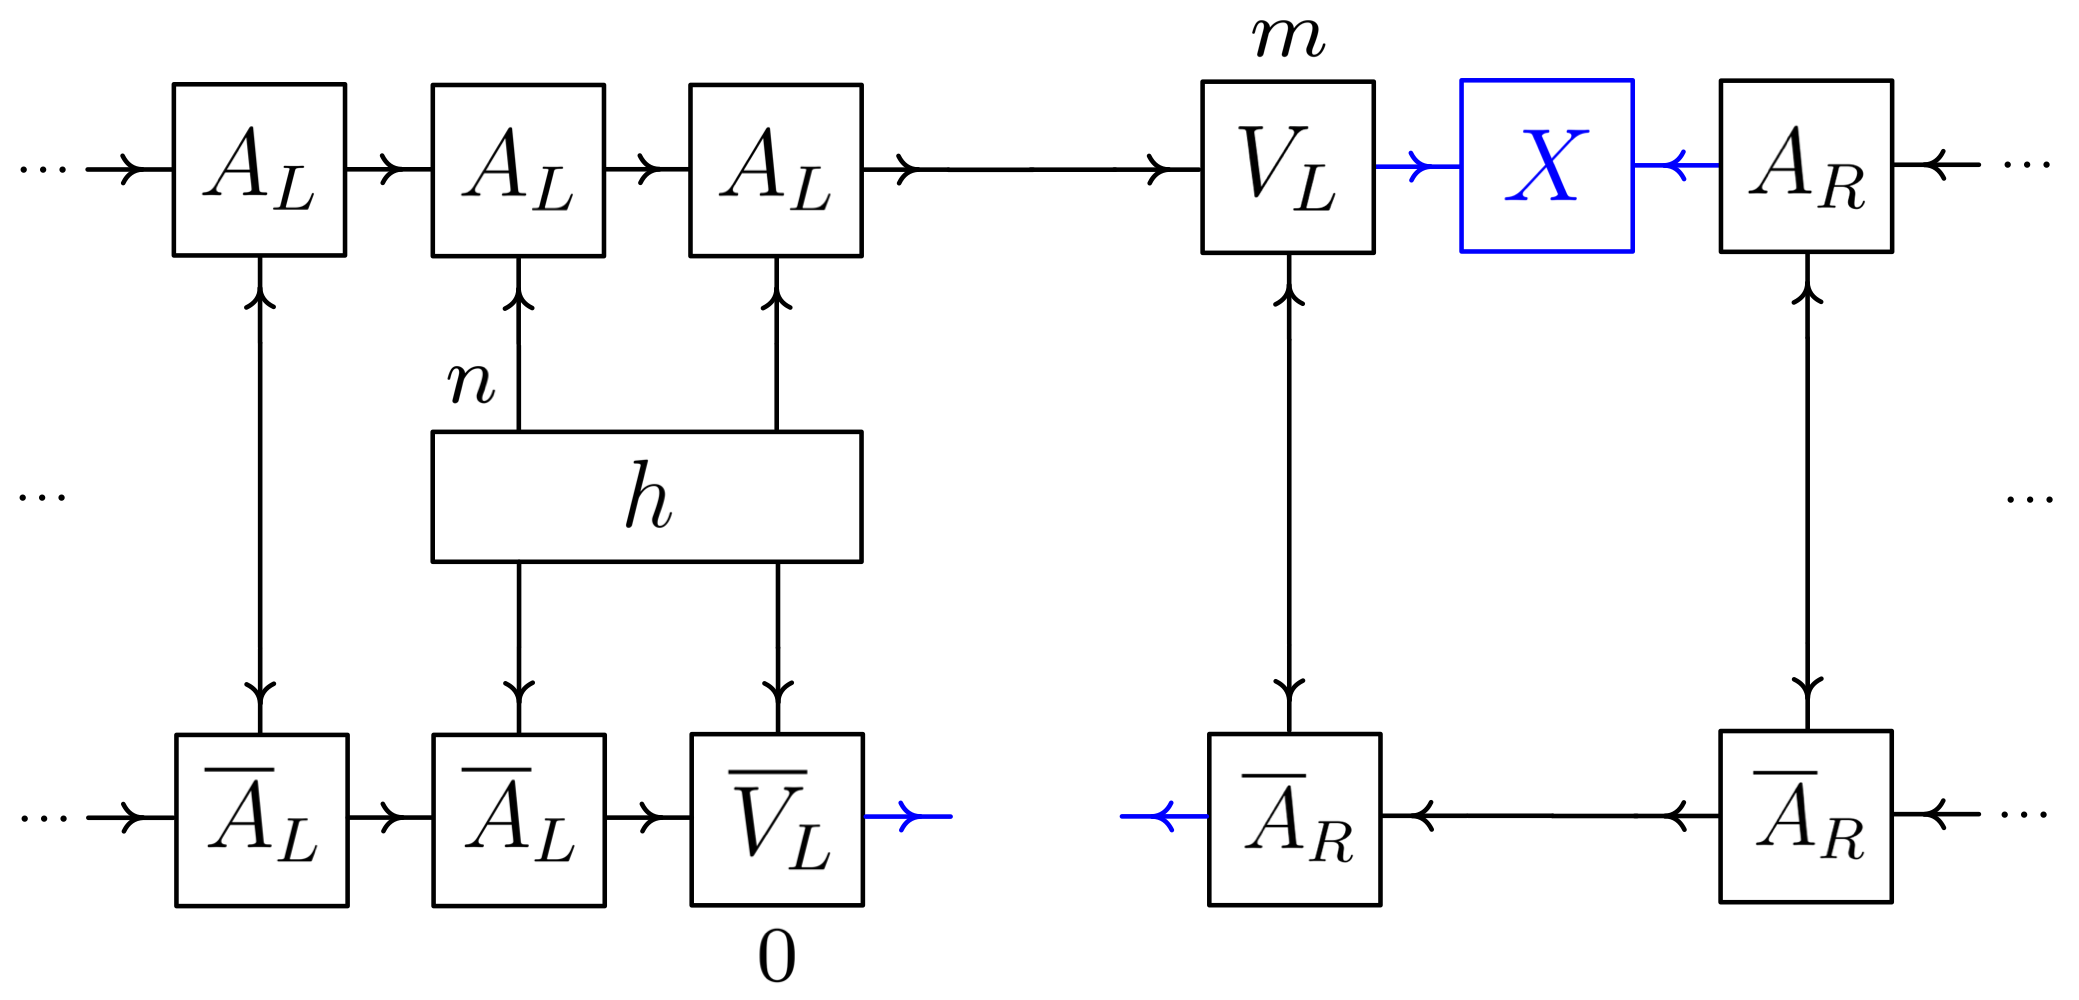
\includegraphics[height=4.5cm]{Heff_p_sum.png}} \hspace{0.2em} .
\end{equation}
\noindent The extensive tensor diagrams for all terms of the double sum \eqref{eq:Heff_p} are shown in appendix \ref{ch:extensive_tensor_network_diagrams}. Some terms vanish in the chosen gauge. In addition to the boundary tensors \eqref{eq:Lh} and \eqref{eq:Rh}, there are also terms involving infinite geometric sums of the mixed transfer matrices
\begin{equation}
	T_{RL} = \sum_s A_R^s \otimes \overline{A^s_L} = \tket{C^{\dagger}}\tbra{C^T} + \mathcal{O}(\vert \lambda_2 \vert) \text{ with } \vert \lambda_2 \vert < 1,
\end{equation}
\begin{equation}
	T_{LR} = \sum_s A_L^s \otimes \overline{A^s_R} = \tket{C}\tbra{\overline{C}} + \mathcal{O}(\vert \lambda_2 \vert) \text{ with } \vert \lambda_2 \vert < 1.
\end{equation}
We explain how these terms can be calculated by picking out one of them:
\begin{align} \label{eq:mixed_geometric_sum}
\begin{split}
	 & e^{-ip} 
	\raisebox{-0.5\height}{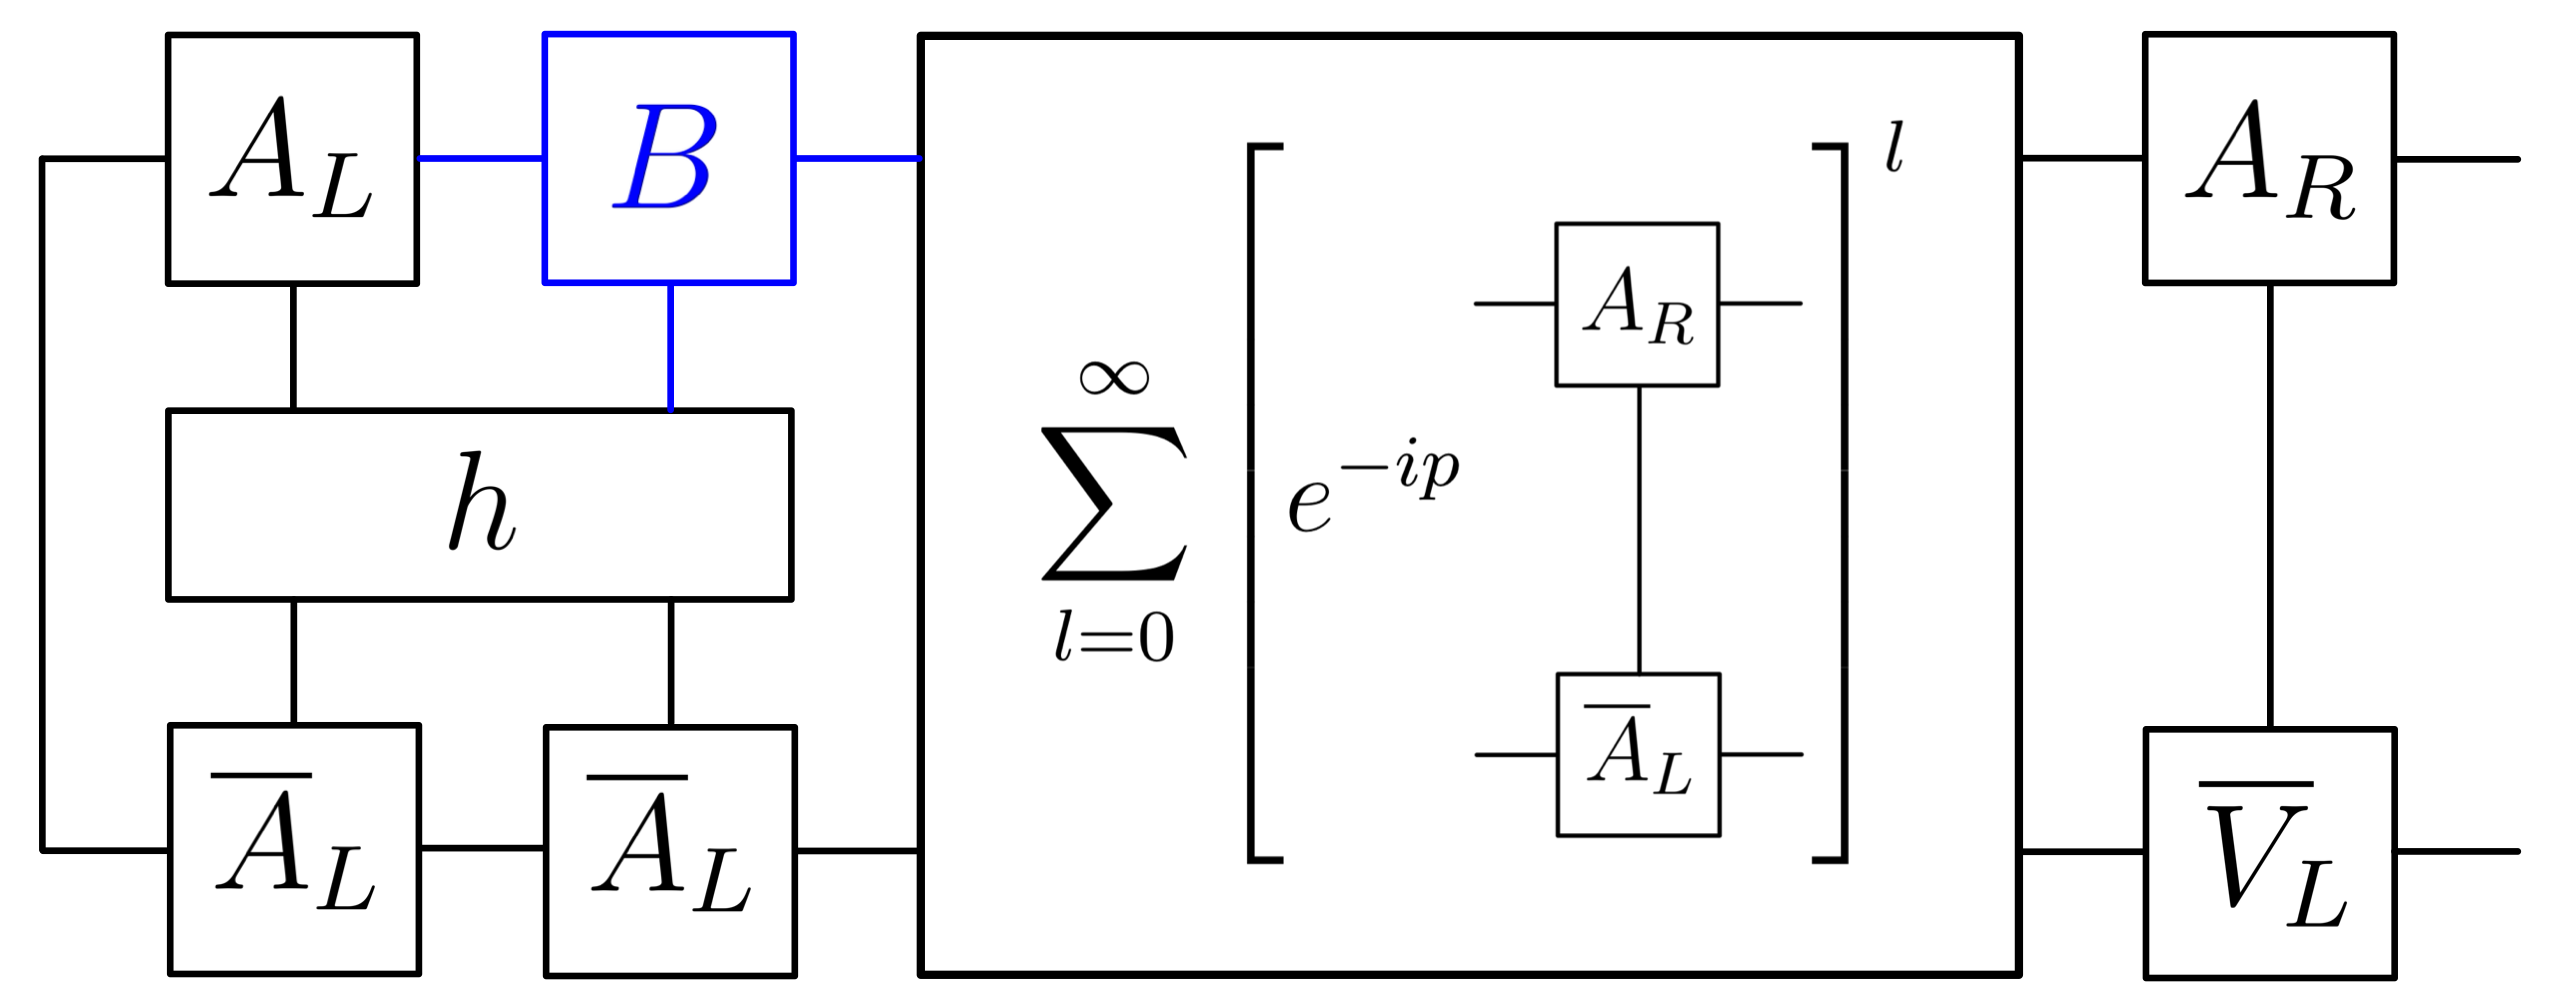
\includegraphics[height=3cm]{LB.png}}  \\
	& = \underbrace{e^{-ip} \tbra{l_B} \sum_{l=0}^{\infty} \left[ e^{-ip} T_{RL} \right]^l}_{\eqqcolon \tbra{L_B}} T_{A_R, \overline{V_L}}.
\end{split}
\end{align}
As for \eqref{eq:Lh} and \eqref{eq:Rh}, we calculate the infinite geometric sum by splitting off the peripheral projector (multiplied by a phase) and using convergence for the residual operator:
\begin{align}
\begin{split} \label{eq:geometric_sum_mixed}
	\sum_{l=0}^{\infty} \left[ e^{-ip} T_{RL} \right]^l &= \left[ \sum_{l=0}^{\infty} e^{-ipl} \right] \tket{C^{\dagger}}\tbra{C^T} + \sum_{l=0}^{\infty} \left[ e^{-ip} T_{RL} - e^{-ip} \tket{C^{\dagger}}\tbra{C^T} \right]^l \\
	&=  \left[ \sum_{l=0}^{\infty} e^{-ipl} \right] \tket{C^{\dagger}}\tbra{C^T} + \left[ \mathbbm{1} - e^{-ip} T_{RL} + e^{-ip} \tket{C^{\dagger}}\tbra{C^T} \right]^{-1}.
\end{split}
\end{align}
The geometric sum $\sum_{l=0}^{\infty} e^{-ipl}$ is divergent. But thanks to the gauge fixing, there is no contribution in the subspace $\tket{C^{\dagger}}\tbra{C^T}$ anyways:
\begin{equation}
	\raisebox{-0.5\height}{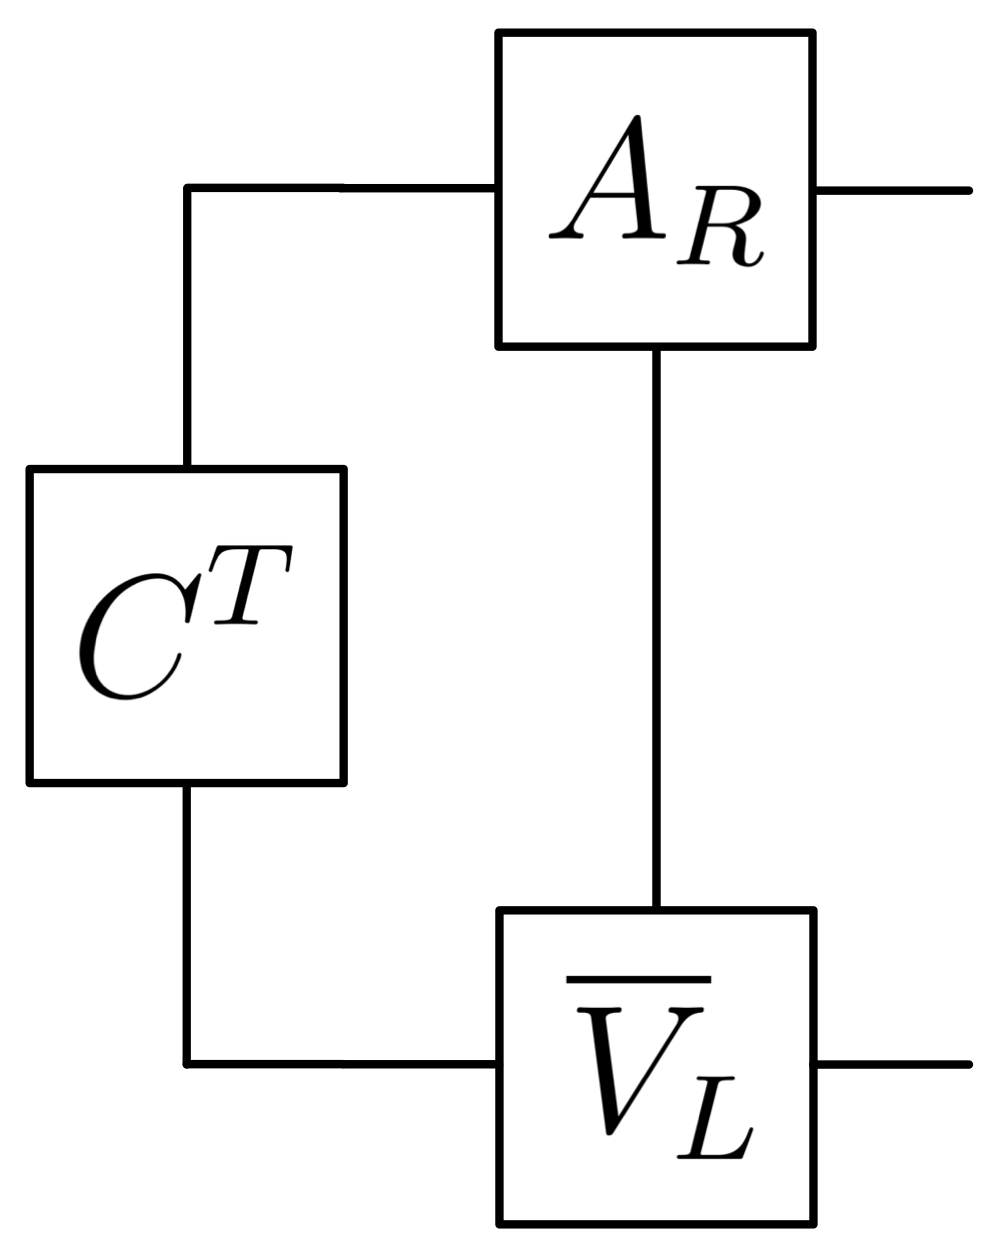
\includegraphics[height=3cm]{CT_AR_VL.png}} 
	= \raisebox{-0.5\height}{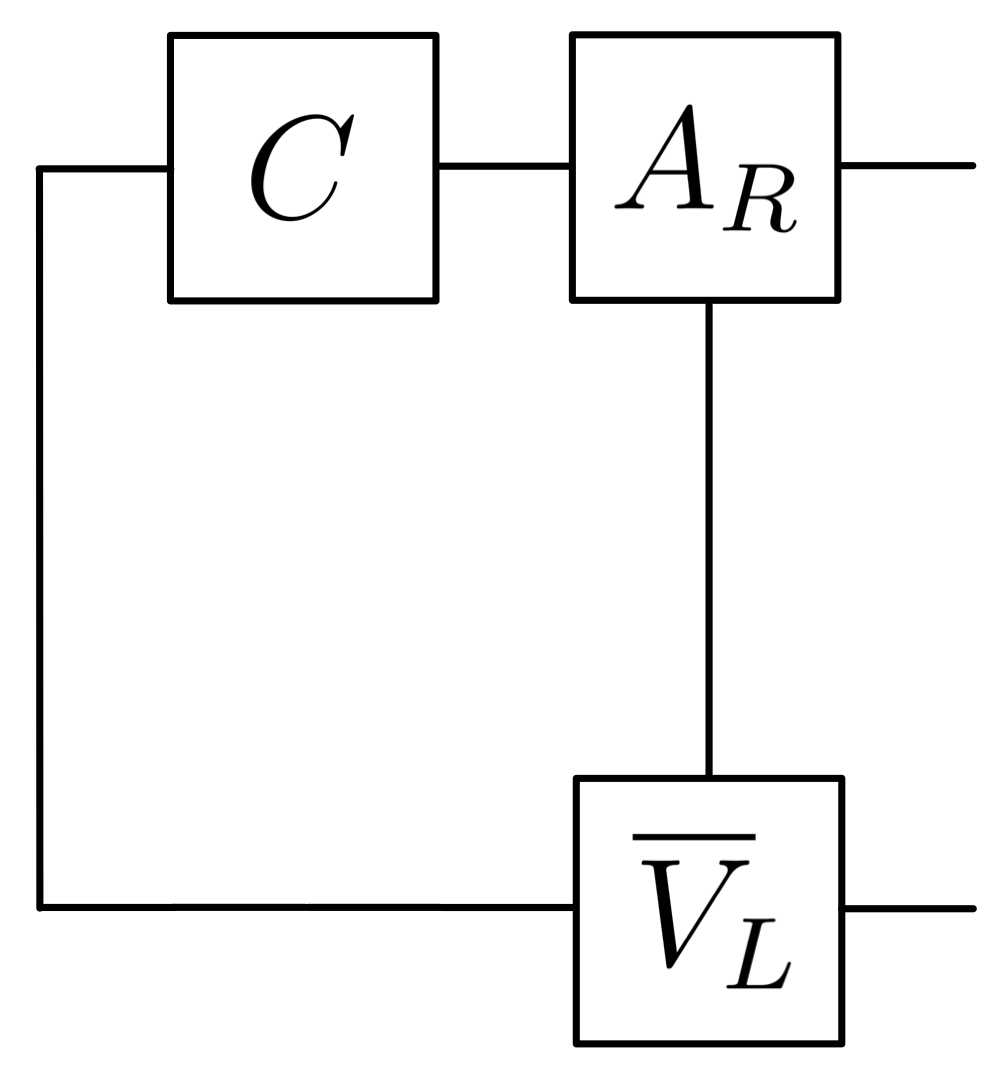
\includegraphics[height=3cm]{C_AR_VL.png}}
	= \raisebox{-0.5\height}{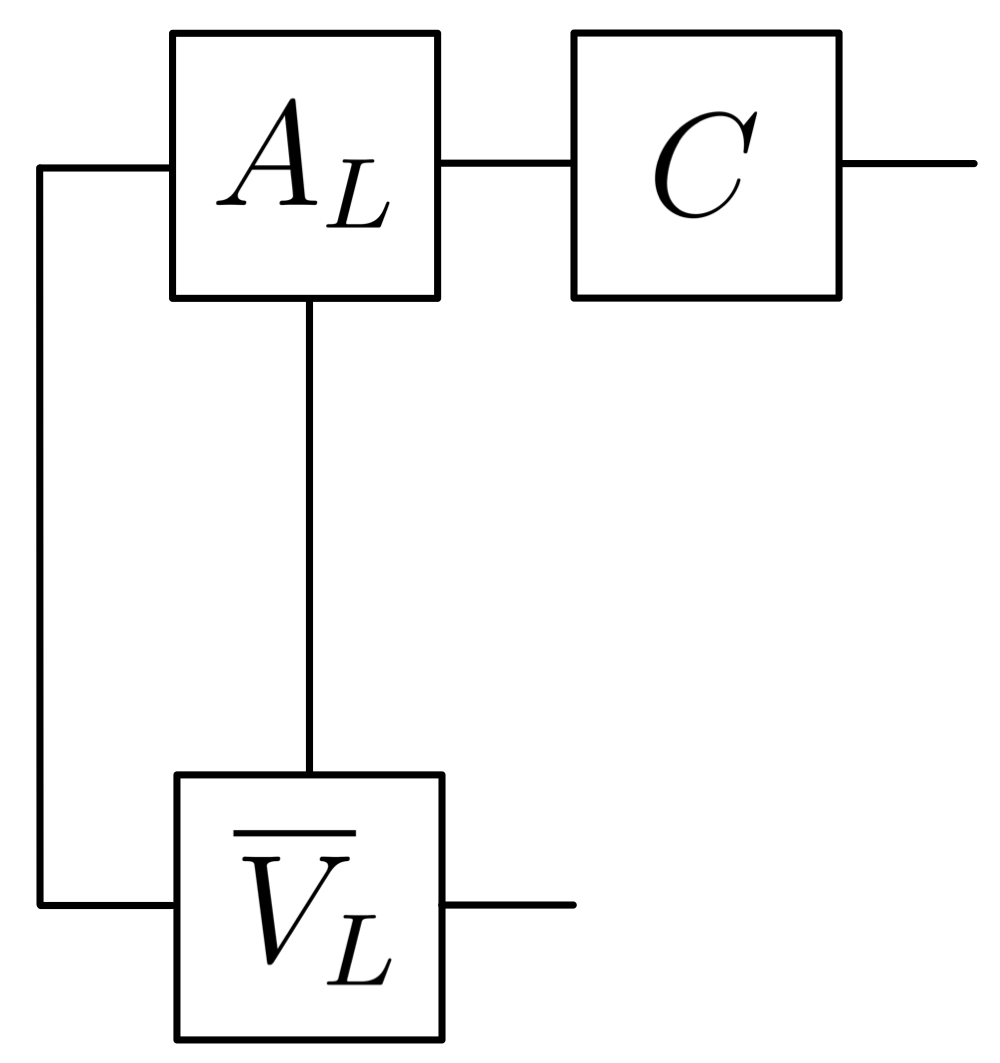
\includegraphics[height=3cm]{AL_C_VL.png}} 
	= 0.
\end{equation}
With this the boundary tensor $\tbra{L_B}$ is obtained from the solution of the following system of linear equations:
\begin{equation}
	\tbra{L_B} \left[ \mathbbm{1} - e^{-ip} T_{RL} + e^{-ip} \tket{C^{\dagger}}\tbra{C^T} \right] = e^{-ip} \tbra{l_B}.
\end{equation}
\noindent Having implemented the whole action of $H_{\mathrm{eff}}(p)$ on $X$ with an iterative Arnoldi method, the optimization \eqref{eq:excitation_minimization} for the lowest lying excitation with momentum $p$ boils down to an iterative ground state search:
\begin{equation} \label{eq:ground_state_H_eff_p}
	H_{\mathrm{eff}}(p) \tket{X} = \epsilon_p \tket{X},
\end{equation}
where $\epsilon_p$ is the energy difference to the ground state. \\[1em]

% topological excitations
\noindent \underline{Topological excitations} \\[0.5em]
\noindent We can also target single topological domain wall excitations with our ansatz \eqref{eq:plane_wave_excitations}, by choosing $A_L$ and $A_R \rightarrow \Tilde{A}_R$ from the two orthogonal symmetry broken ground states. The only difference in the algorithm concerns the mixed transfer matrices $T_{\Tilde{R}L}$ and $T_{L\Tilde{R}}$. Since they have spectral radius strictly smaller than one (otherwise the two symmetry broken ground states would not be orthogonal), the corresponding infinite geometric sums can be computed with the full inverse:
\begin{equation}
	\sum_{l=0}^{\infty} \left[ e^{-ip} T_{\Tilde{R}L} \right]^l  = \left[ \mathbbm{1} - e^{-ip} T_{\Tilde{R}L} \right]^{-1}.
\end{equation}
As a second peculiarity, multiplying $\Tilde{A}_R$ with a phase $e^{i \phi}$ shifts the momentum $p \rightarrow p + \phi$. We fix it unambiguously by ensuring that the dominant eigenvalue of $T_{\Tilde{R}L}$ is positive. \\[1em]

% benchmark
\noindent \underline{Benchmark} \\[0.5em]
\noindent In total, we have presented an algorithm that variationally finds elementary quasiparticle excitations on top of a VUMPS ground state. These excitations may be of local or topological nature. They describe plane waves with definite momentum $p$ and excitation energy $\epsilon_p$. By solving the effective Hamiltonian eigenequation \eqref{eq:ground_state_H_eff_p} with an iterative Lanczos method for multiple momenta $p$ within the first Brillouin zone $(- \pi, \pi ]$, we can infer a dispersion relation. For the TFI model, we can compare it to the exact one:
\begin{equation}
	\epsilon_p \overset{J = 1}{=} 2\sqrt{g^2 - 2 g \cos(p) + 1} \:\:.
\end{equation}
The result is shown in figure \ref{fig:uexcitations_dispersion}, again for the transverse field values $g = 0.5$ (symmetry broken phase), $g = 1.0$ (critical point) and $g = 1.5$ (unordered phase). Within the given energy resolution, all optimized pairs $(p, \epsilon_p)$ lie precisely on the dispersion curve. The persistence of sharp quasiparticle excitations at criticality is a special feature of the TFI model, due to its exact mapping to free fermions, as discussed in section \ref{sec:tfi_exact_solution}. In general, the excitations of critical quantum many body systems have a more complex, collective structure.
\begin{figure}[t]
  \centering
  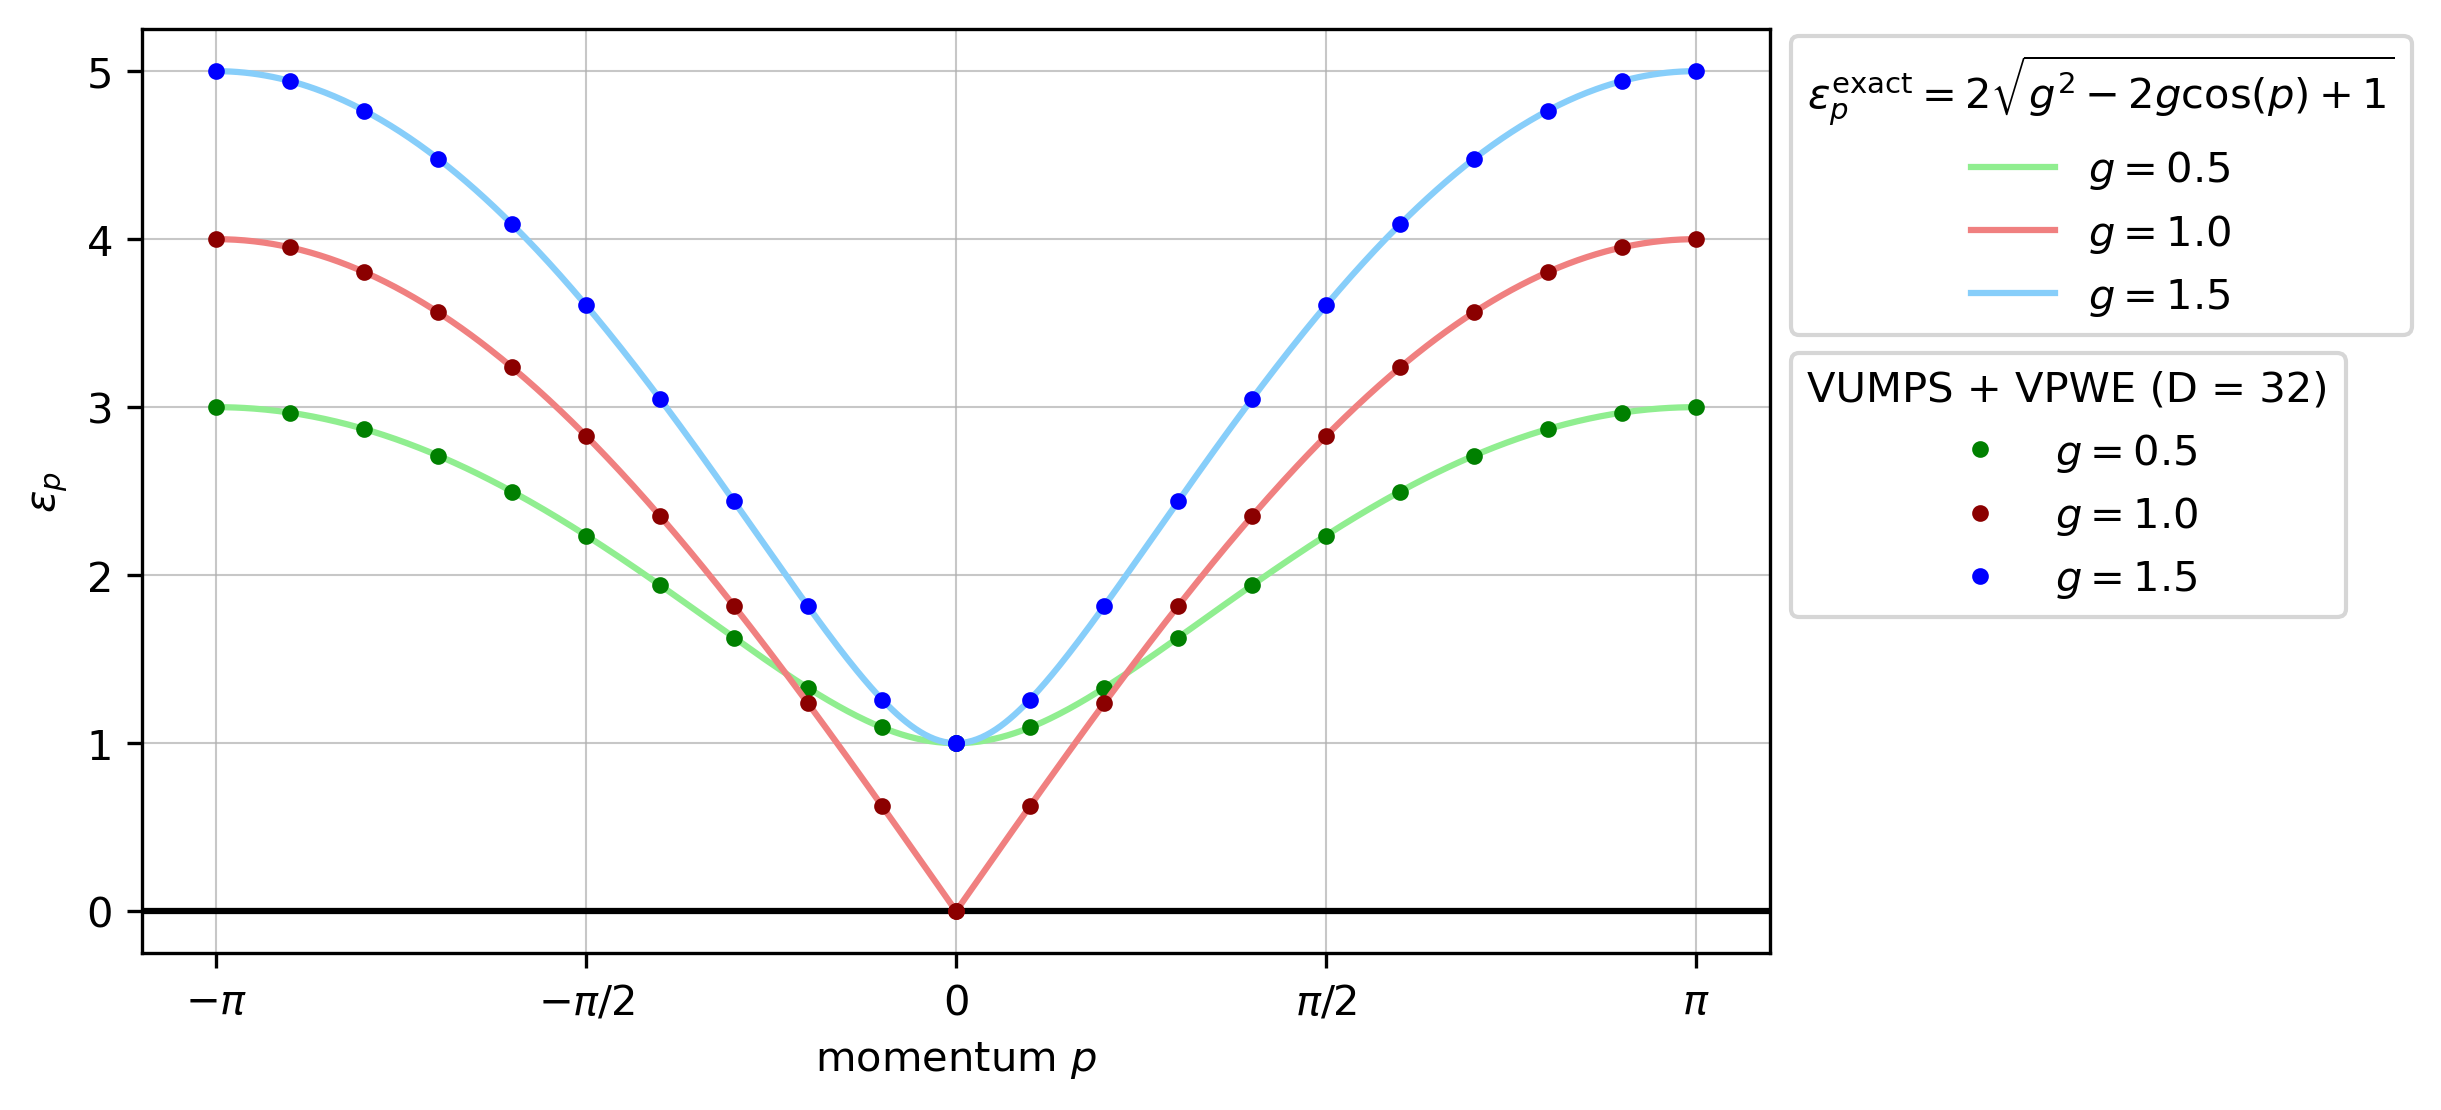
\includegraphics[width=1.0\linewidth]{uexcitations_dispersion.png}
  \caption{TFI benchmark for variational plane wave excitations (VPWE) on top of a uMPS ground state. Optimization of the quasiparticle ansatz $\ket{\psi_p(X; A)}$ for the lowest lying excitation of the Hamiltonian boils down to the ground state equation $H_{\mathrm{eff}}(p) \tket{X} = \epsilon_p \tket{X}$. We solve it with an iterative Lanczos method for multiple momenta $p$ within the first Brillouin zone. The results lie on the exact dispersion curve for all three values of $g$, even at criticality.}
\label{fig:uexcitations_dispersion}
\end{figure}